 \documentclass[a4paper,10pt]{article}
\usepackage[utf8]{inputenc}
\usepackage[bitstream-charter]{mathdesign}
\usepackage{ragged2e}
\usepackage[spanish]{babel}
\usepackage{anysize}
\marginsize{1.5cm}{1.5cm}{2cm}{2cm}
\usepackage{amsmath}
\usepackage{hyperref}
\usepackage{textcomp,gensymb}
\usepackage{float}
\usepackage[table,xcdraw]{xcolor}
\usepackage{lipsum}
\usepackage{graphicx}
\usepackage{caption}
\usepackage{subcaption}
\usepackage[table,xcdraw]{xcolor}

\usepackage{mathrsfs}


\usepackage{fancyhdr} %Poner encabezado
\pagestyle{fancy} % Poner encabezado
\fancyhead[LE,RO]{} % Encabezado en páginas par
\fancyhead[LO,RE]{Universidad Industrial de Santander} % Encabezado en páginas impar
\rhead{Semillero de astronomía AstrAra} %número de página

%\lhead{\begin{picture}(0,0) \put(0,0){\includegraphics[width=20mm]{2}} \end{picture}}

%\rhead{\begin{picture}(0,0) \put(-86.7,0){\includegraphics[width=30mm]{1}} \end{picture}}




\usepackage{url}
\usepackage[font=small,labelfont=bf]{caption}
\usepackage{multicol}
\setlength\columnsep{18pt}
\renewenvironment{abstract}
 {\par\noindent\textbf{\abstractname}\ \ignorespaces \\}
 {\par\noindent\medskip}
 



%-----------------------------------------------------------------------------------------------------------------------------------------


\graphicspath{{graphics/}{graphics/arch/}{Graphics/}{./}} % Look in these folders for graphics
%
% Put here some packages required or/and some personnal commands
%
%
\lhead{\begin{picture}(0,0) \put(0,0){
\includegraphics[width=35mm]{uis.png} \hspace{4mm} 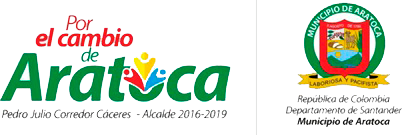
\includegraphics[width=50mm]{Imagenes/5143aa2c-2917-4ffe-adf6-727908e18acb.png}} \end{picture}}

\begin{document}

\begin{center}
\Large\textbf{{Informe de actividades semillero de astronomía AstrAra}}
\vspace{0.4cm}

\normalsize
\textit{ }

\vspace{0.1cm}

\textit{\small{Escuela de Física, Grupo Halley}\\
\small{Universidad Industrial de Santander}}
\medskip
\medskip
\normalsize


\end{center}
%-----------------------------------------------------------------------------------------------------------------------------------------
\line(1,0){550}
\vspace{0.1cm}



%-----------------------------------------------------------------------------------------------------------------------------------------


\noindent El presente informe de actividades da a conocer el registro de las dinámicas y temáticas realizadas en las tres instituciones educativas elegidas por el Municipio de Aratoca - Santander, con el fin de soportar el total de las 45 horas estipuladas en el convenio entre la alcaldía de Aratoca y la Universidad Industrial de Santander, enfocado hacia el proyecto AstrAra. El contenido de actividades se divide en tres (3) grandes secciones (La Luz, El Sistema Solar y El Sistema Local Sol-Tierra-Luna) cada una pensada para 5 horas. Estas actividades se realizaron en paralelo en cada colegio (completando 15 horas en una jornada) durante tres jornadas, es decir, tres encuentros, cada uno en días diferentes con las respectivas instituciones, para un total de 45 horas. Para cada jornada, la organización interna de los instructores, se estableció tal que cada pareja de instructores se trasladara a su respectiva institución y diera inicio de actividades en el horario de 7:30 am a 1:00 pm, donde se tiene en cuenta cada día media hora dedicada al descanso de los estudiantes, (dicho descanso no está incluido en las horas de planeación presentadas). Abarcando así las 15 horas por cada día ya mencionadas (5 en cada colegio).
%Por otro lado, en todas las sesiones de los colegios, se trabajó con dos grupos de estudiantes, uno de ellos estudiantes de cuarto y quinto de primaria y el otro de noveno y décimo grado, con actividades similares, lo que cambiaba de estas sesiones solo es la forma en que se explican algunos conceptos ya que los estudiantes de noveno y décimo tienen mucho más bagaje en conocimientos de ciencia que los estudiantes más chicos.

%blablablalbablablabl%
\section{La luz}

\begin{figure}[H]
    \centering
    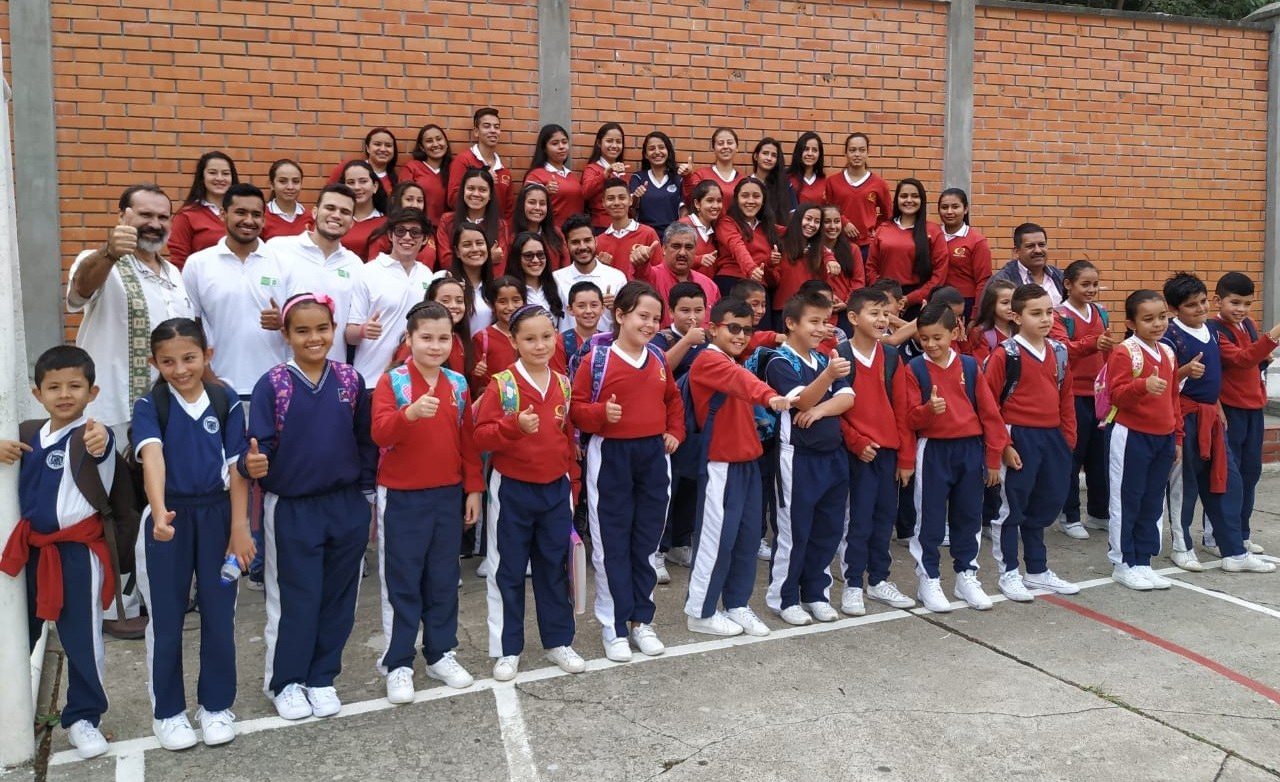
\includegraphics[width=8.0cm]{Imagenes/foto2.jpeg}
    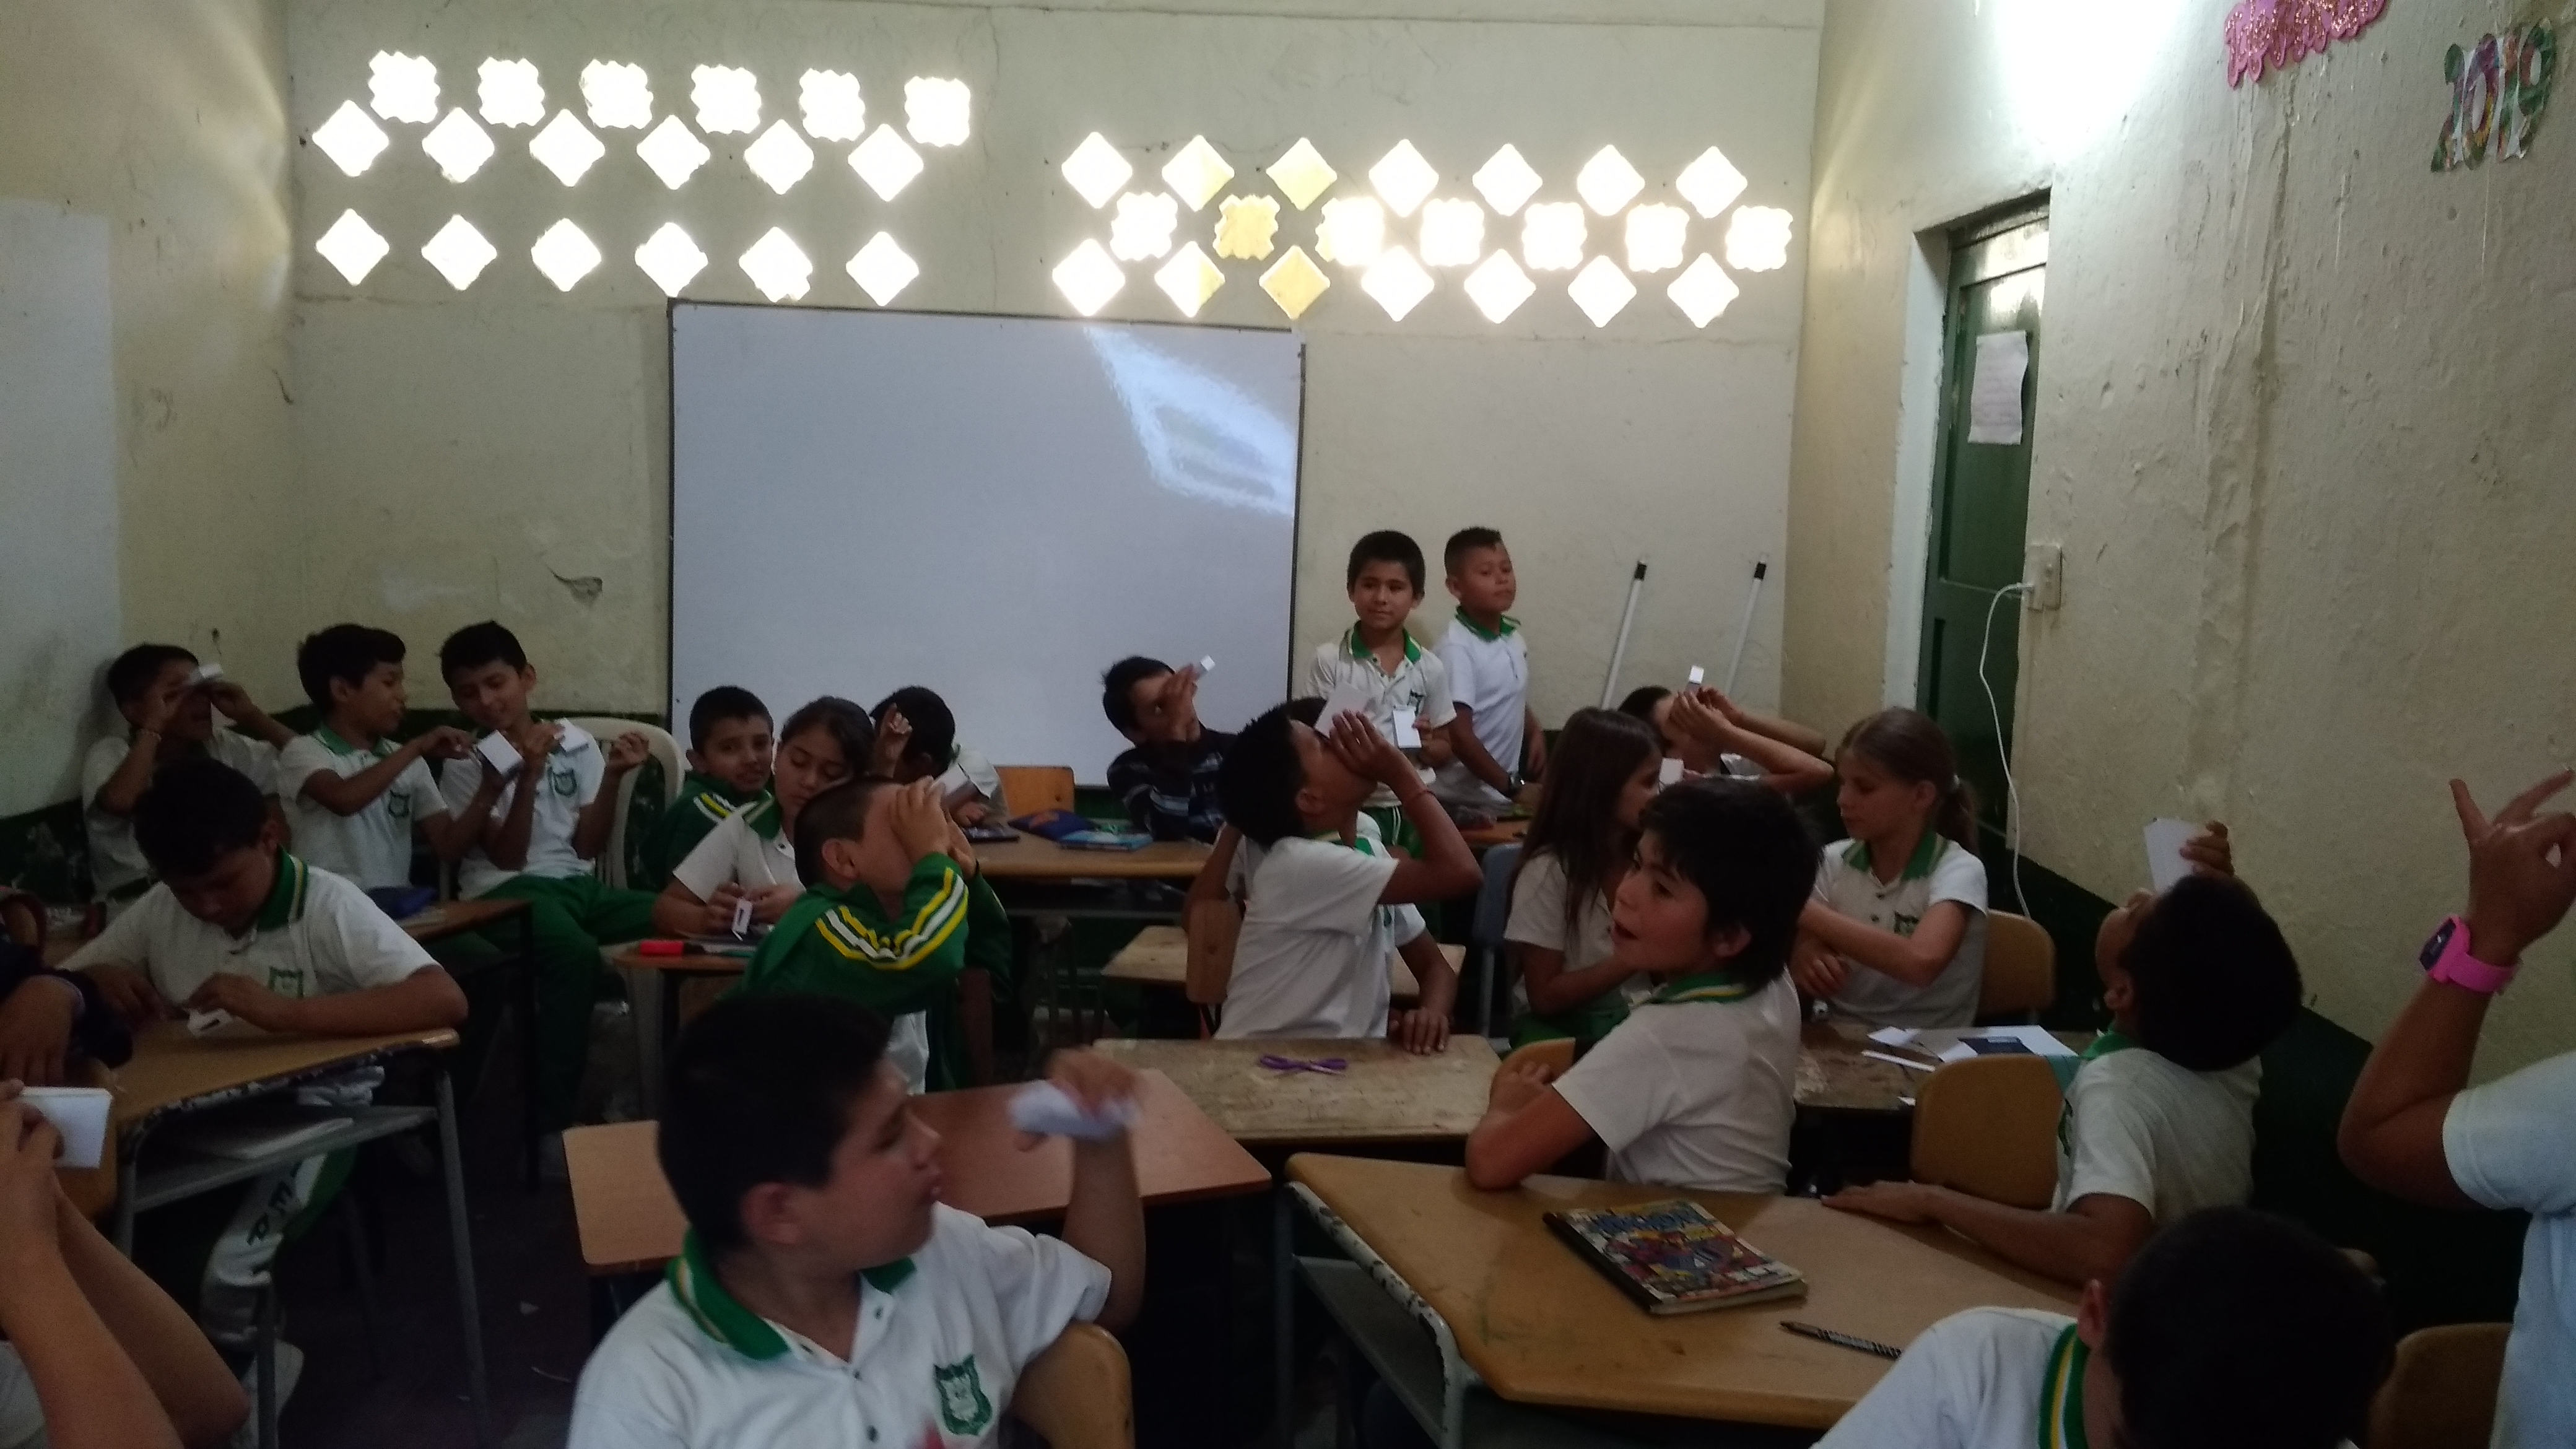
\includegraphics[width=8.7cm]{Imagenes/portico.jpg}
    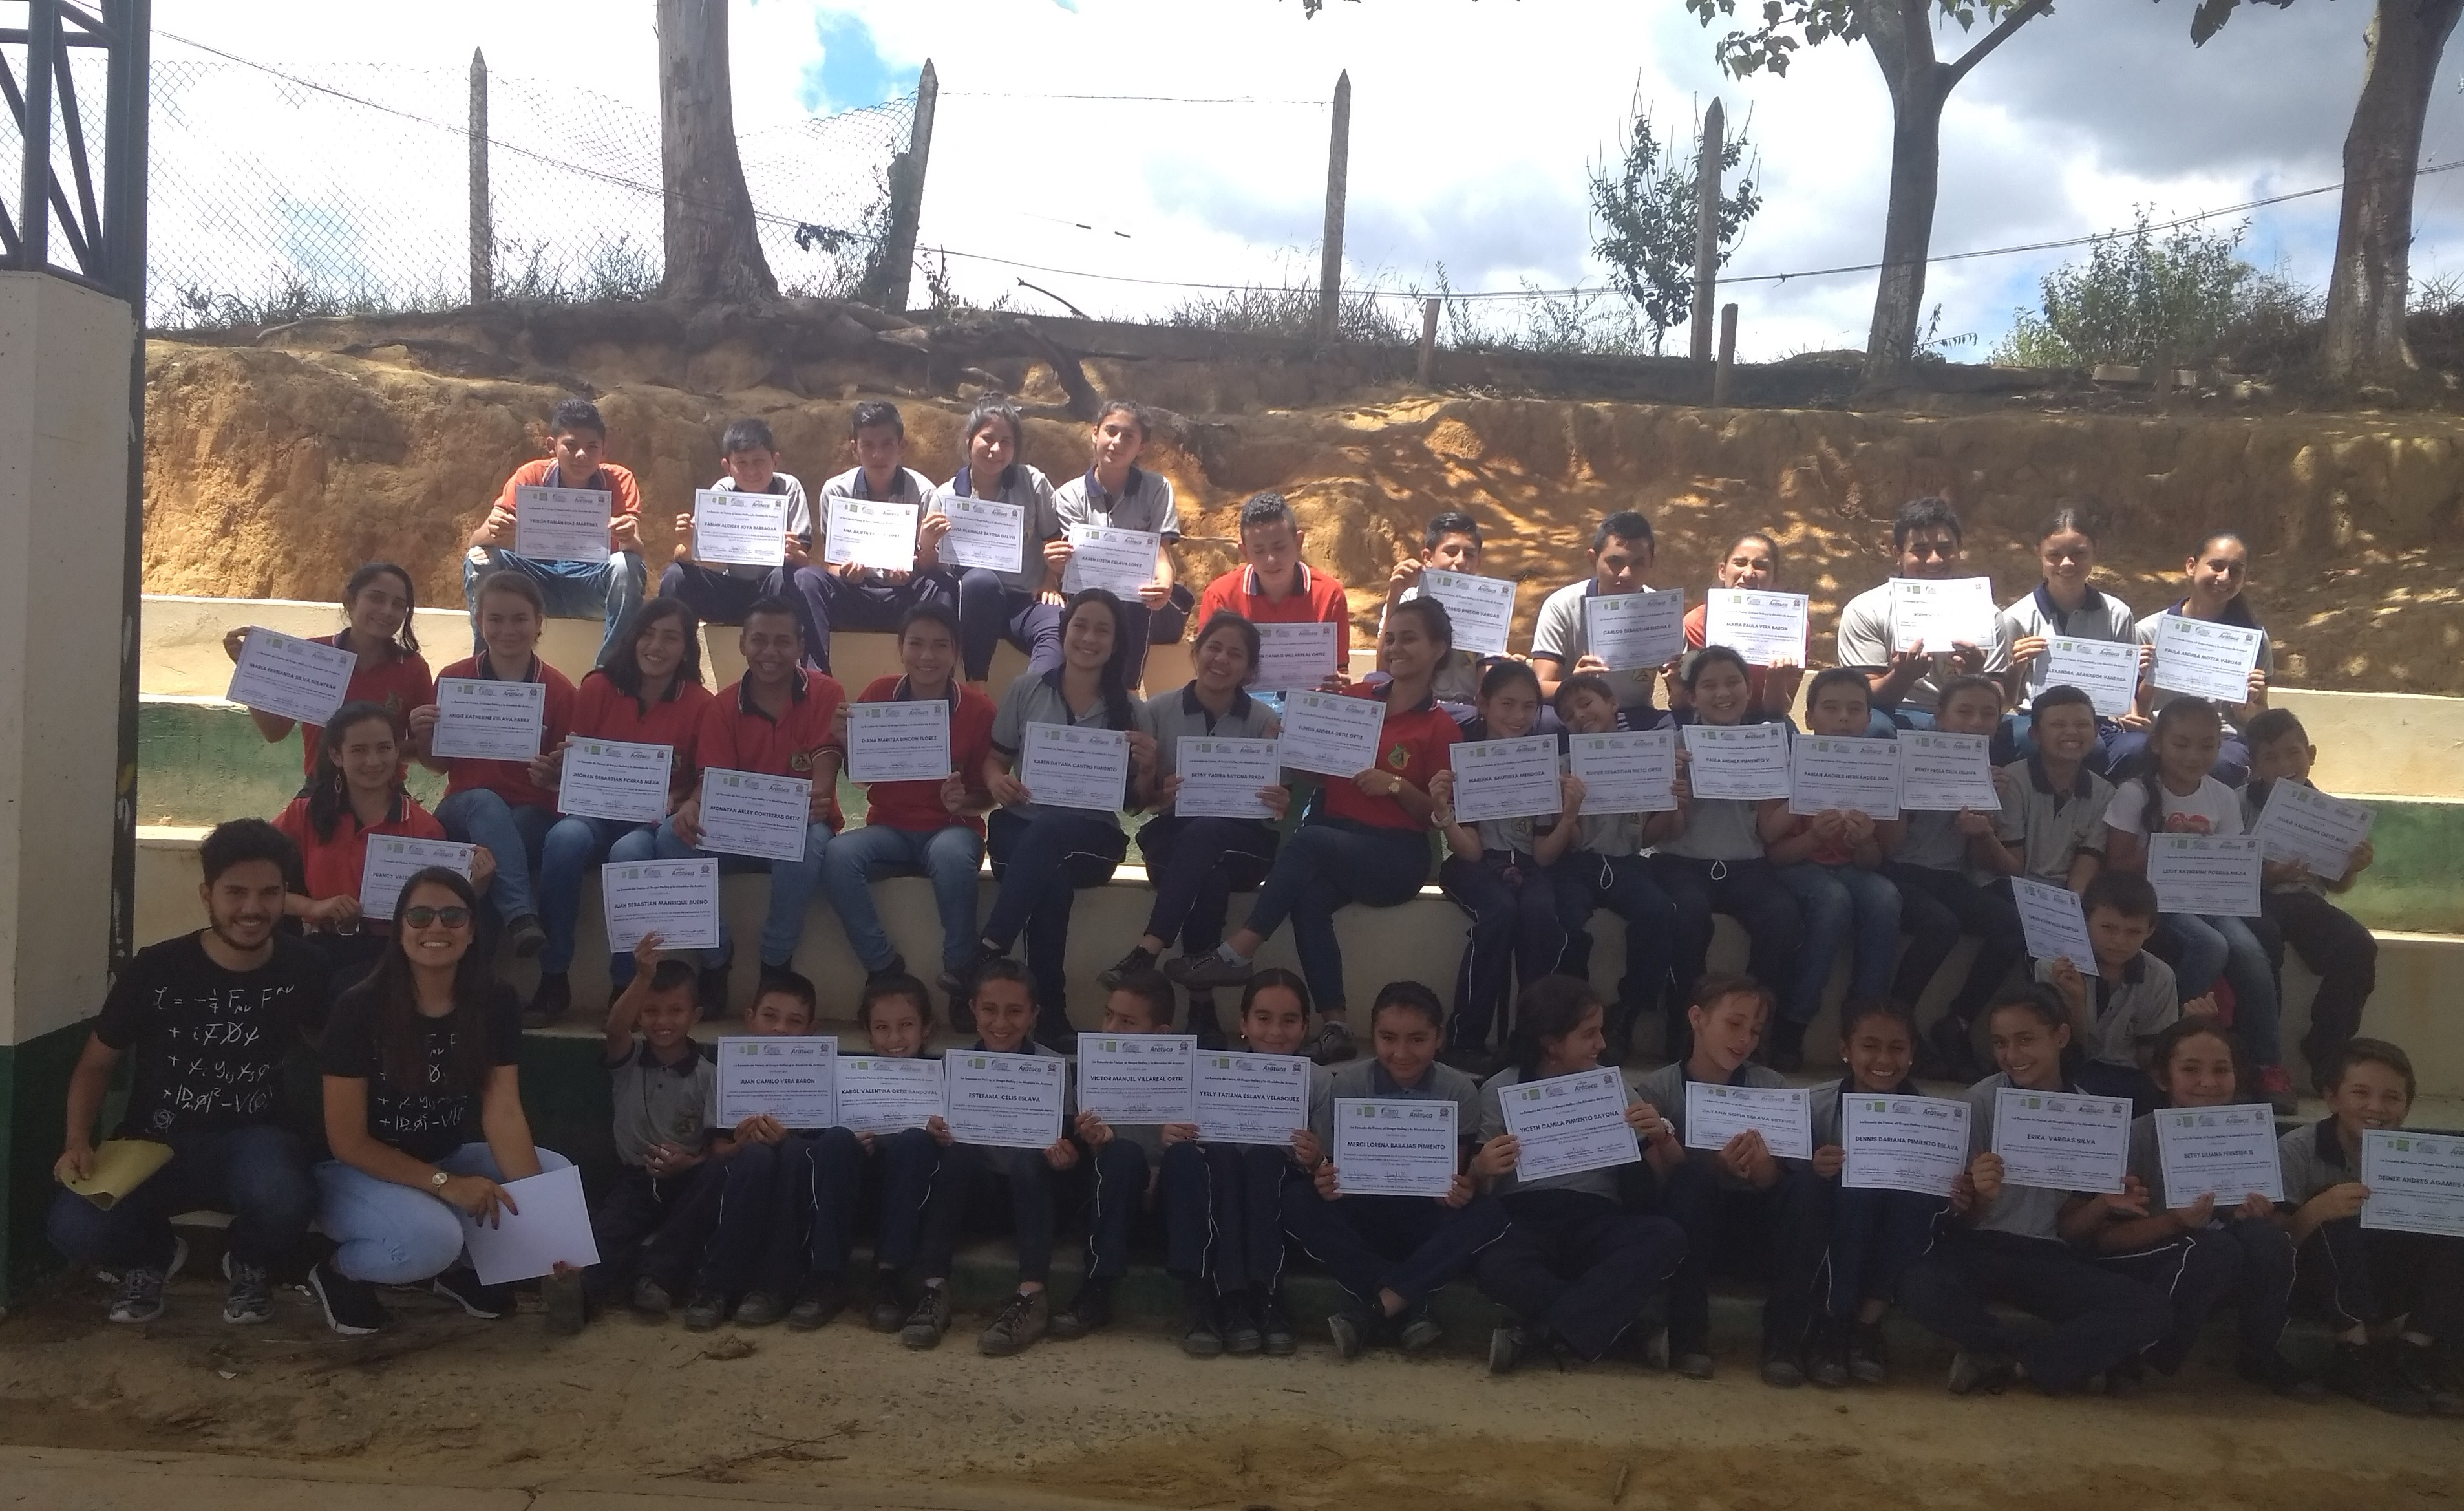
\includegraphics[width=8.5cm]{Imagenes/certificadoclave.jpg}
    \caption{Estudiantes del Colegio San Luis (Esquina superior izquierda), Institución Educativa el Pórtico (Esquina superior derecha) e Institución Educativa Clavellinas (Parte inferior). }
\end{figure}

\noindent Las secciones correspondientes a este tema se trabajaron en dos grupos separados: primaria con los grados cuarto y quinto; y bachillerato con los grados noveno y décimo. En los dos grupos se abordó desde la teoría y se complementó con actividades didácticas, las temáticas estudiadas fueron las siguientes:

\begin{itemize}
    \item ¿Qué es la luz?
    \item El espectro de la luz
    \item Polarización y dispersión
    \item Construcción de un espectroscopio con un CD viejo
    \item Nociones sobre astronomía moderna
\end{itemize}
\vspace{3mm}
\subsection{Actividades desarrolladas}
\noindent \textbf{¿Qué es la luz? (40 minutos)}\\

\noindent En esta temática se discutió la noción de luz, la importancia de la luz en la vida cotidiana y un poco de historia sobre los avances en la comprensión de la luz y sus fenómenos. Posteriormente se abordó el comportamiento de la luz como onda y con el fin de explicar la relación entre la frecuencia y la energía se desarrollo una actividad con tiza, dicha actividad consistía en dibujar ondas en el piso con diferentes colores de tiza (azul y rojo) y diferentes frecuencias, a continuación algunos niños recorrían las ondas hasta terminar el recorrido con la condición de que todos debían llegar al mismo tiempo. Al final, se preguntó a los niños ¿Cuál de ellos se encontraba más cansado? y ¿Por qué creen que sucedió esto?. Finalmente se explicó que el niño que recorrió la onda con mayor frecuencia (color azul) se sintió más cansado al terminar la actividad pues esta onda es muy energética y presenta muchas oscilaciones, mientras que el que recorrió la onda roja no va a sentirse tan cansado.

\begin{figure}[H]
    \centering
    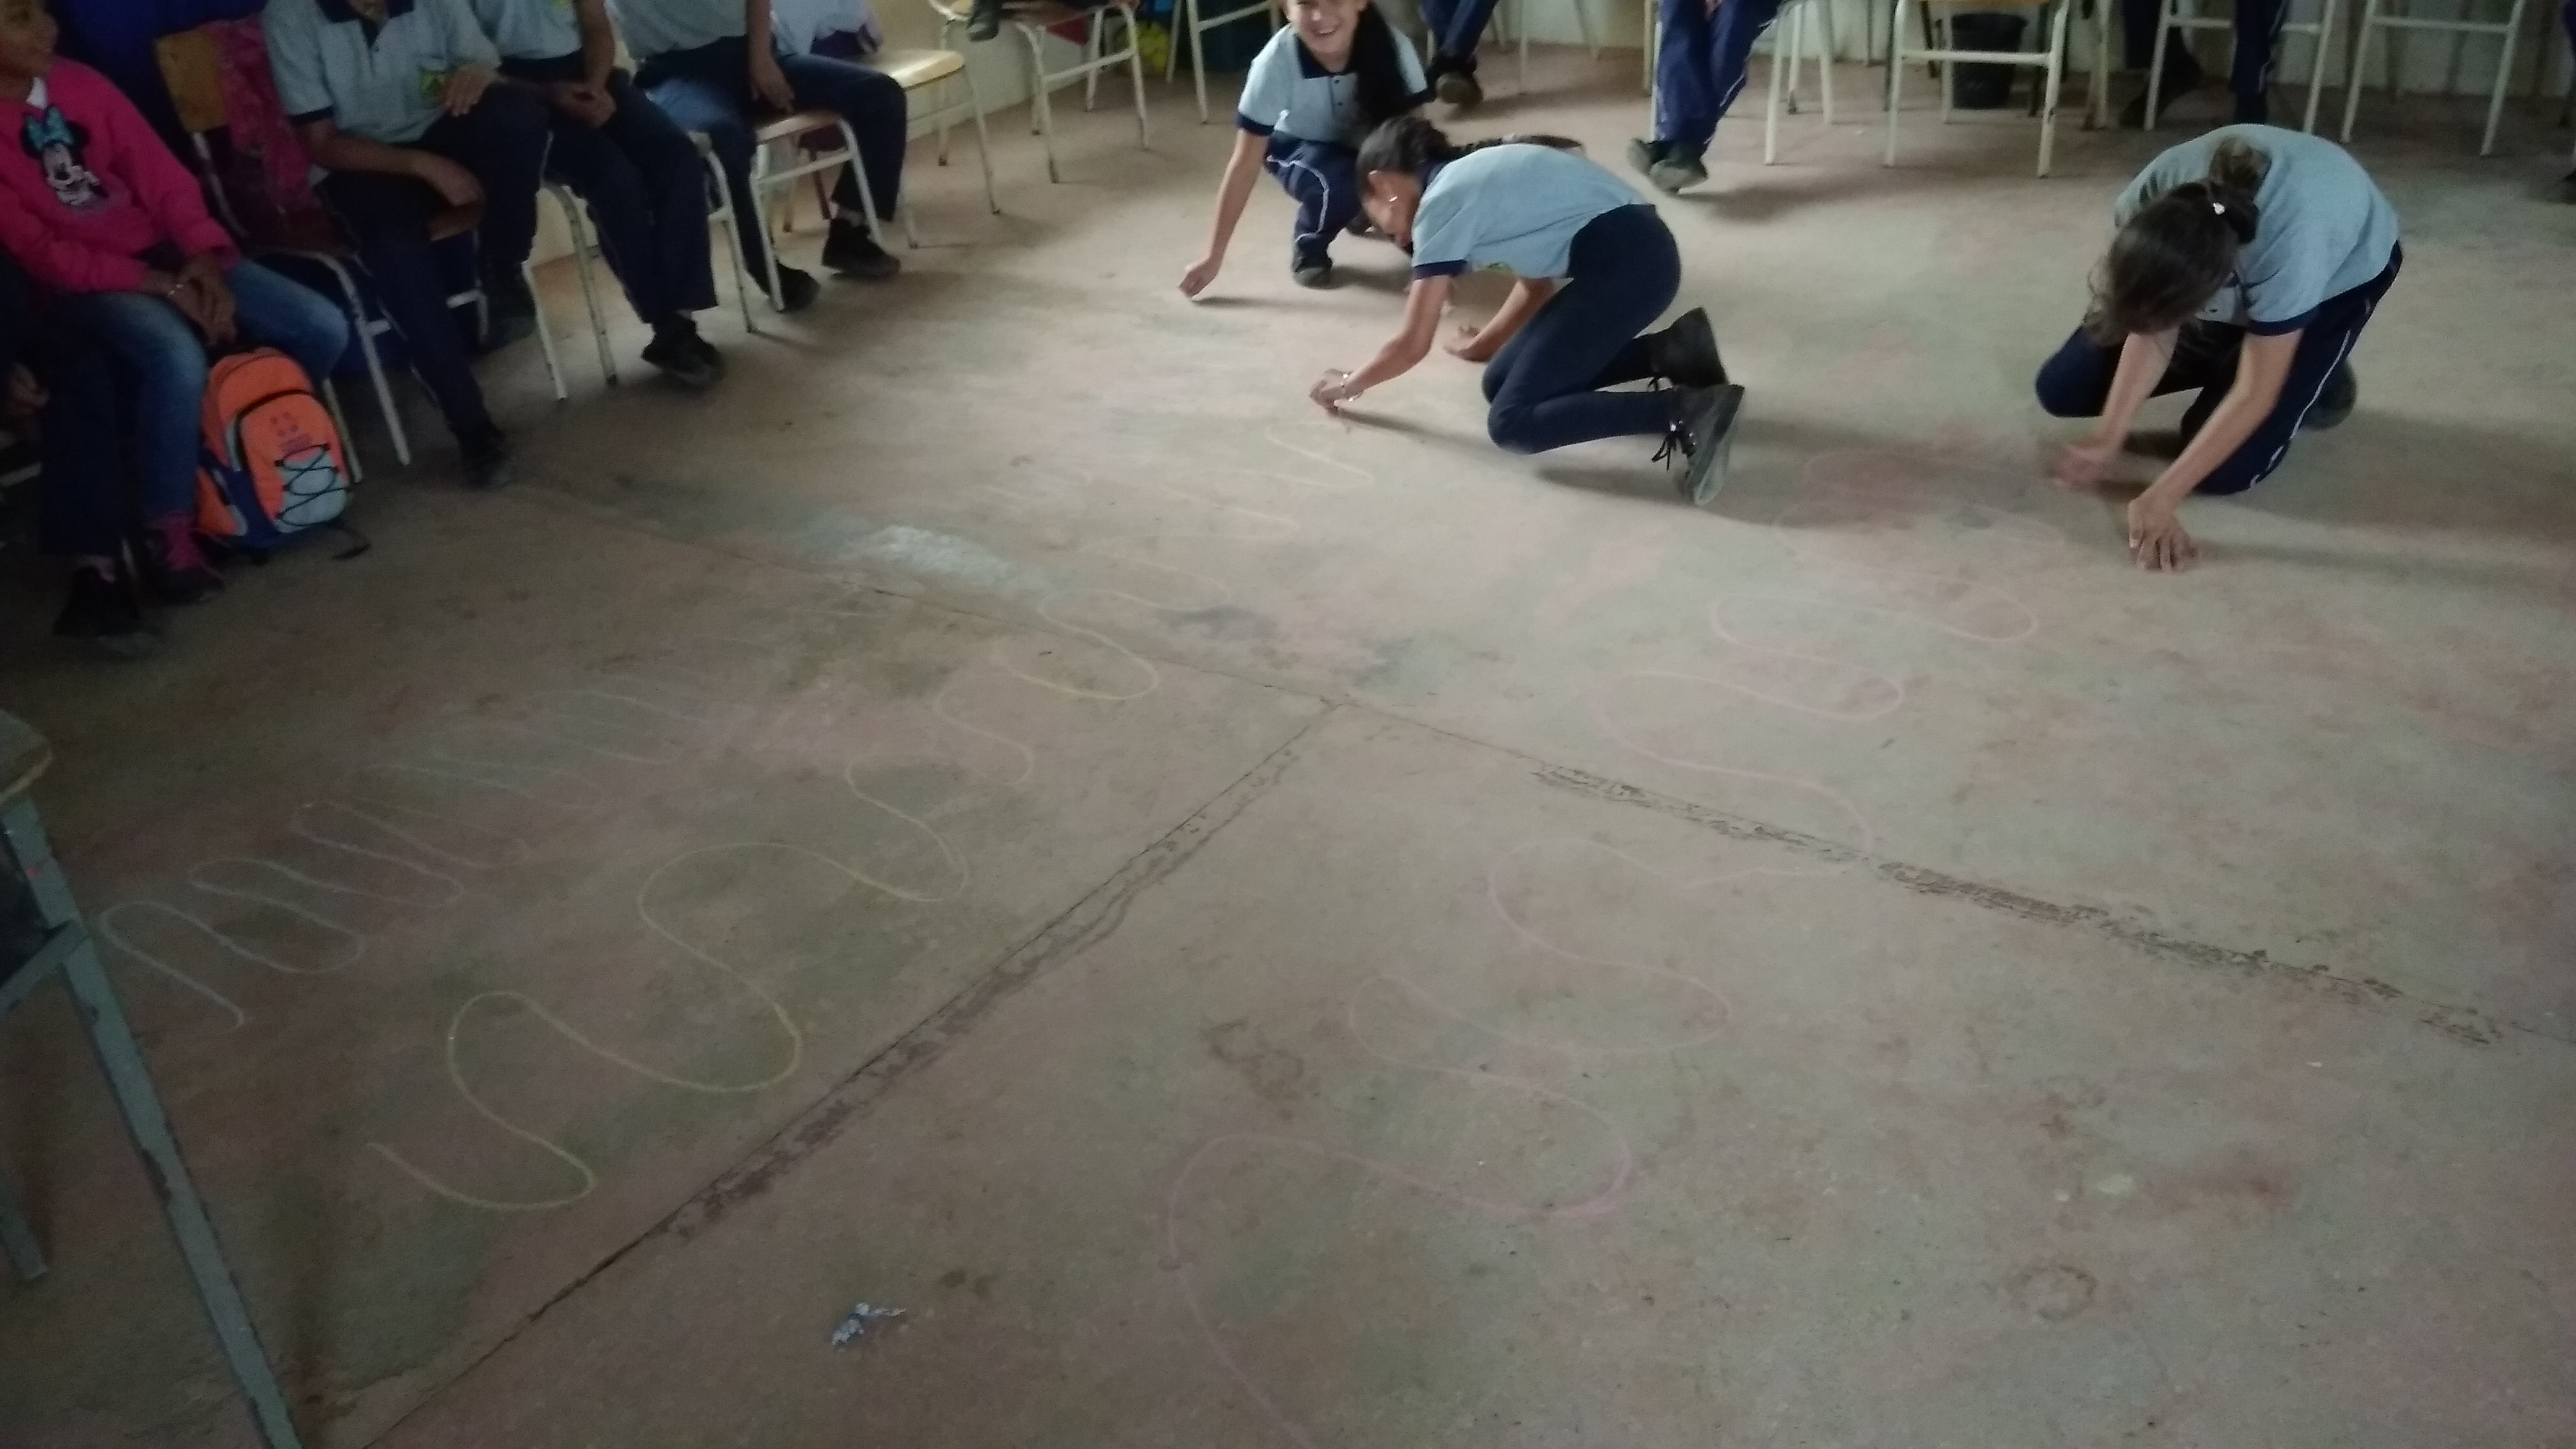
\includegraphics[width = 8.3 cm]{Imagenes/ondas1clave.jpg}
    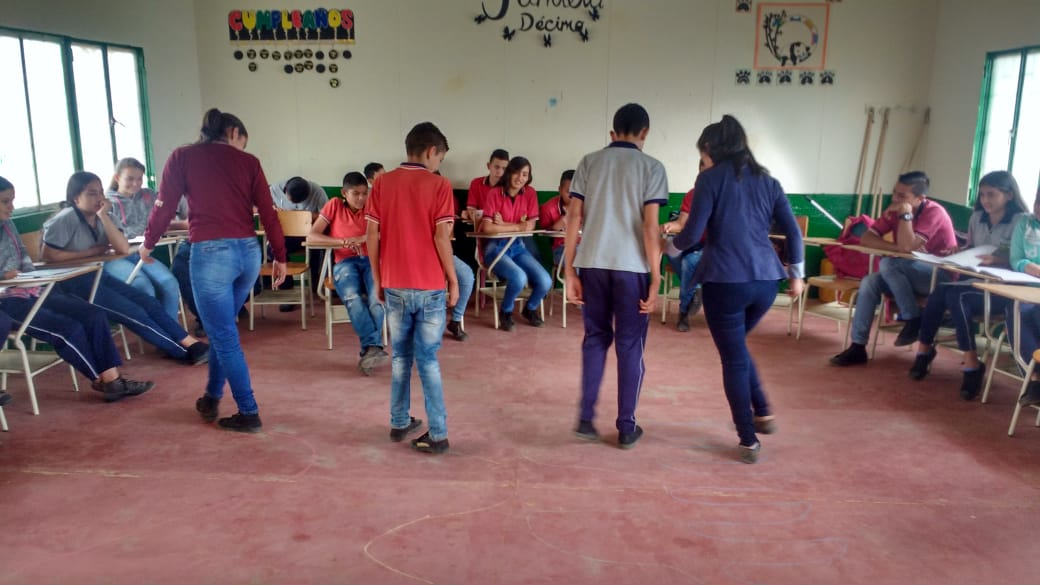
\includegraphics[width = 8.4 cm]{Imagenes/luz3.jpeg}
     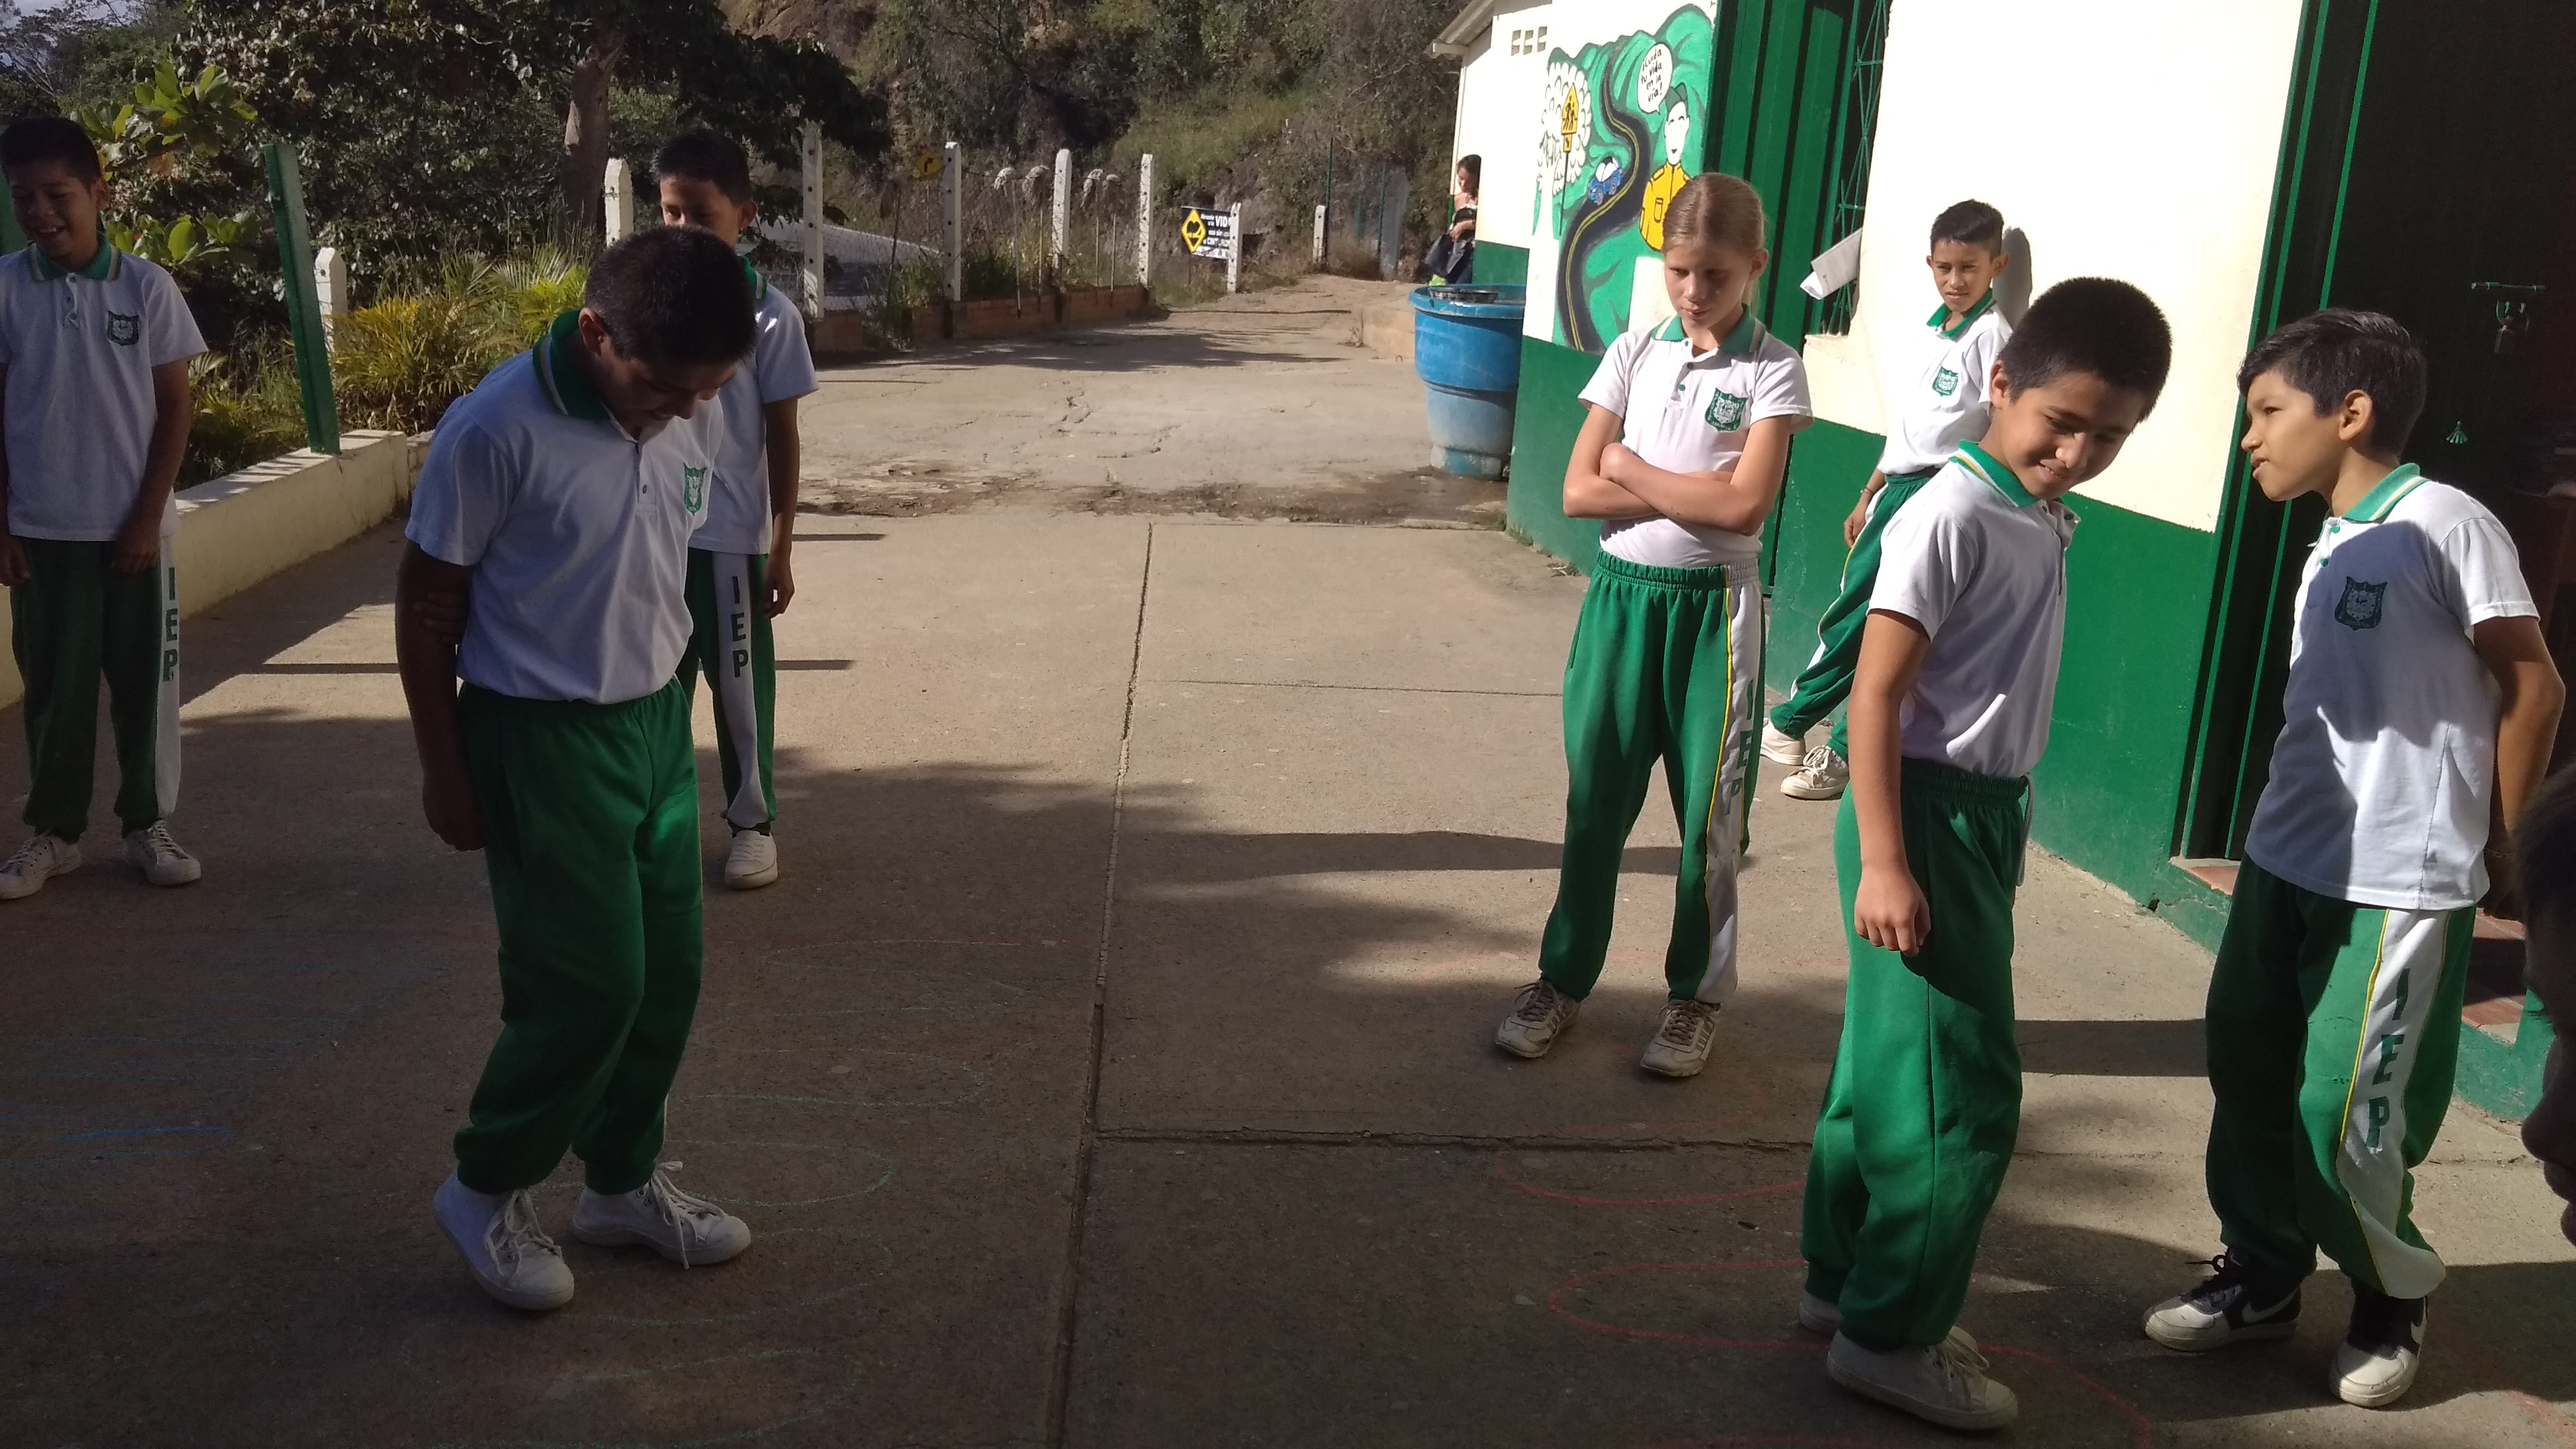
\includegraphics[width = 8.3 cm]{Imagenes/onda2portico.jpg}
     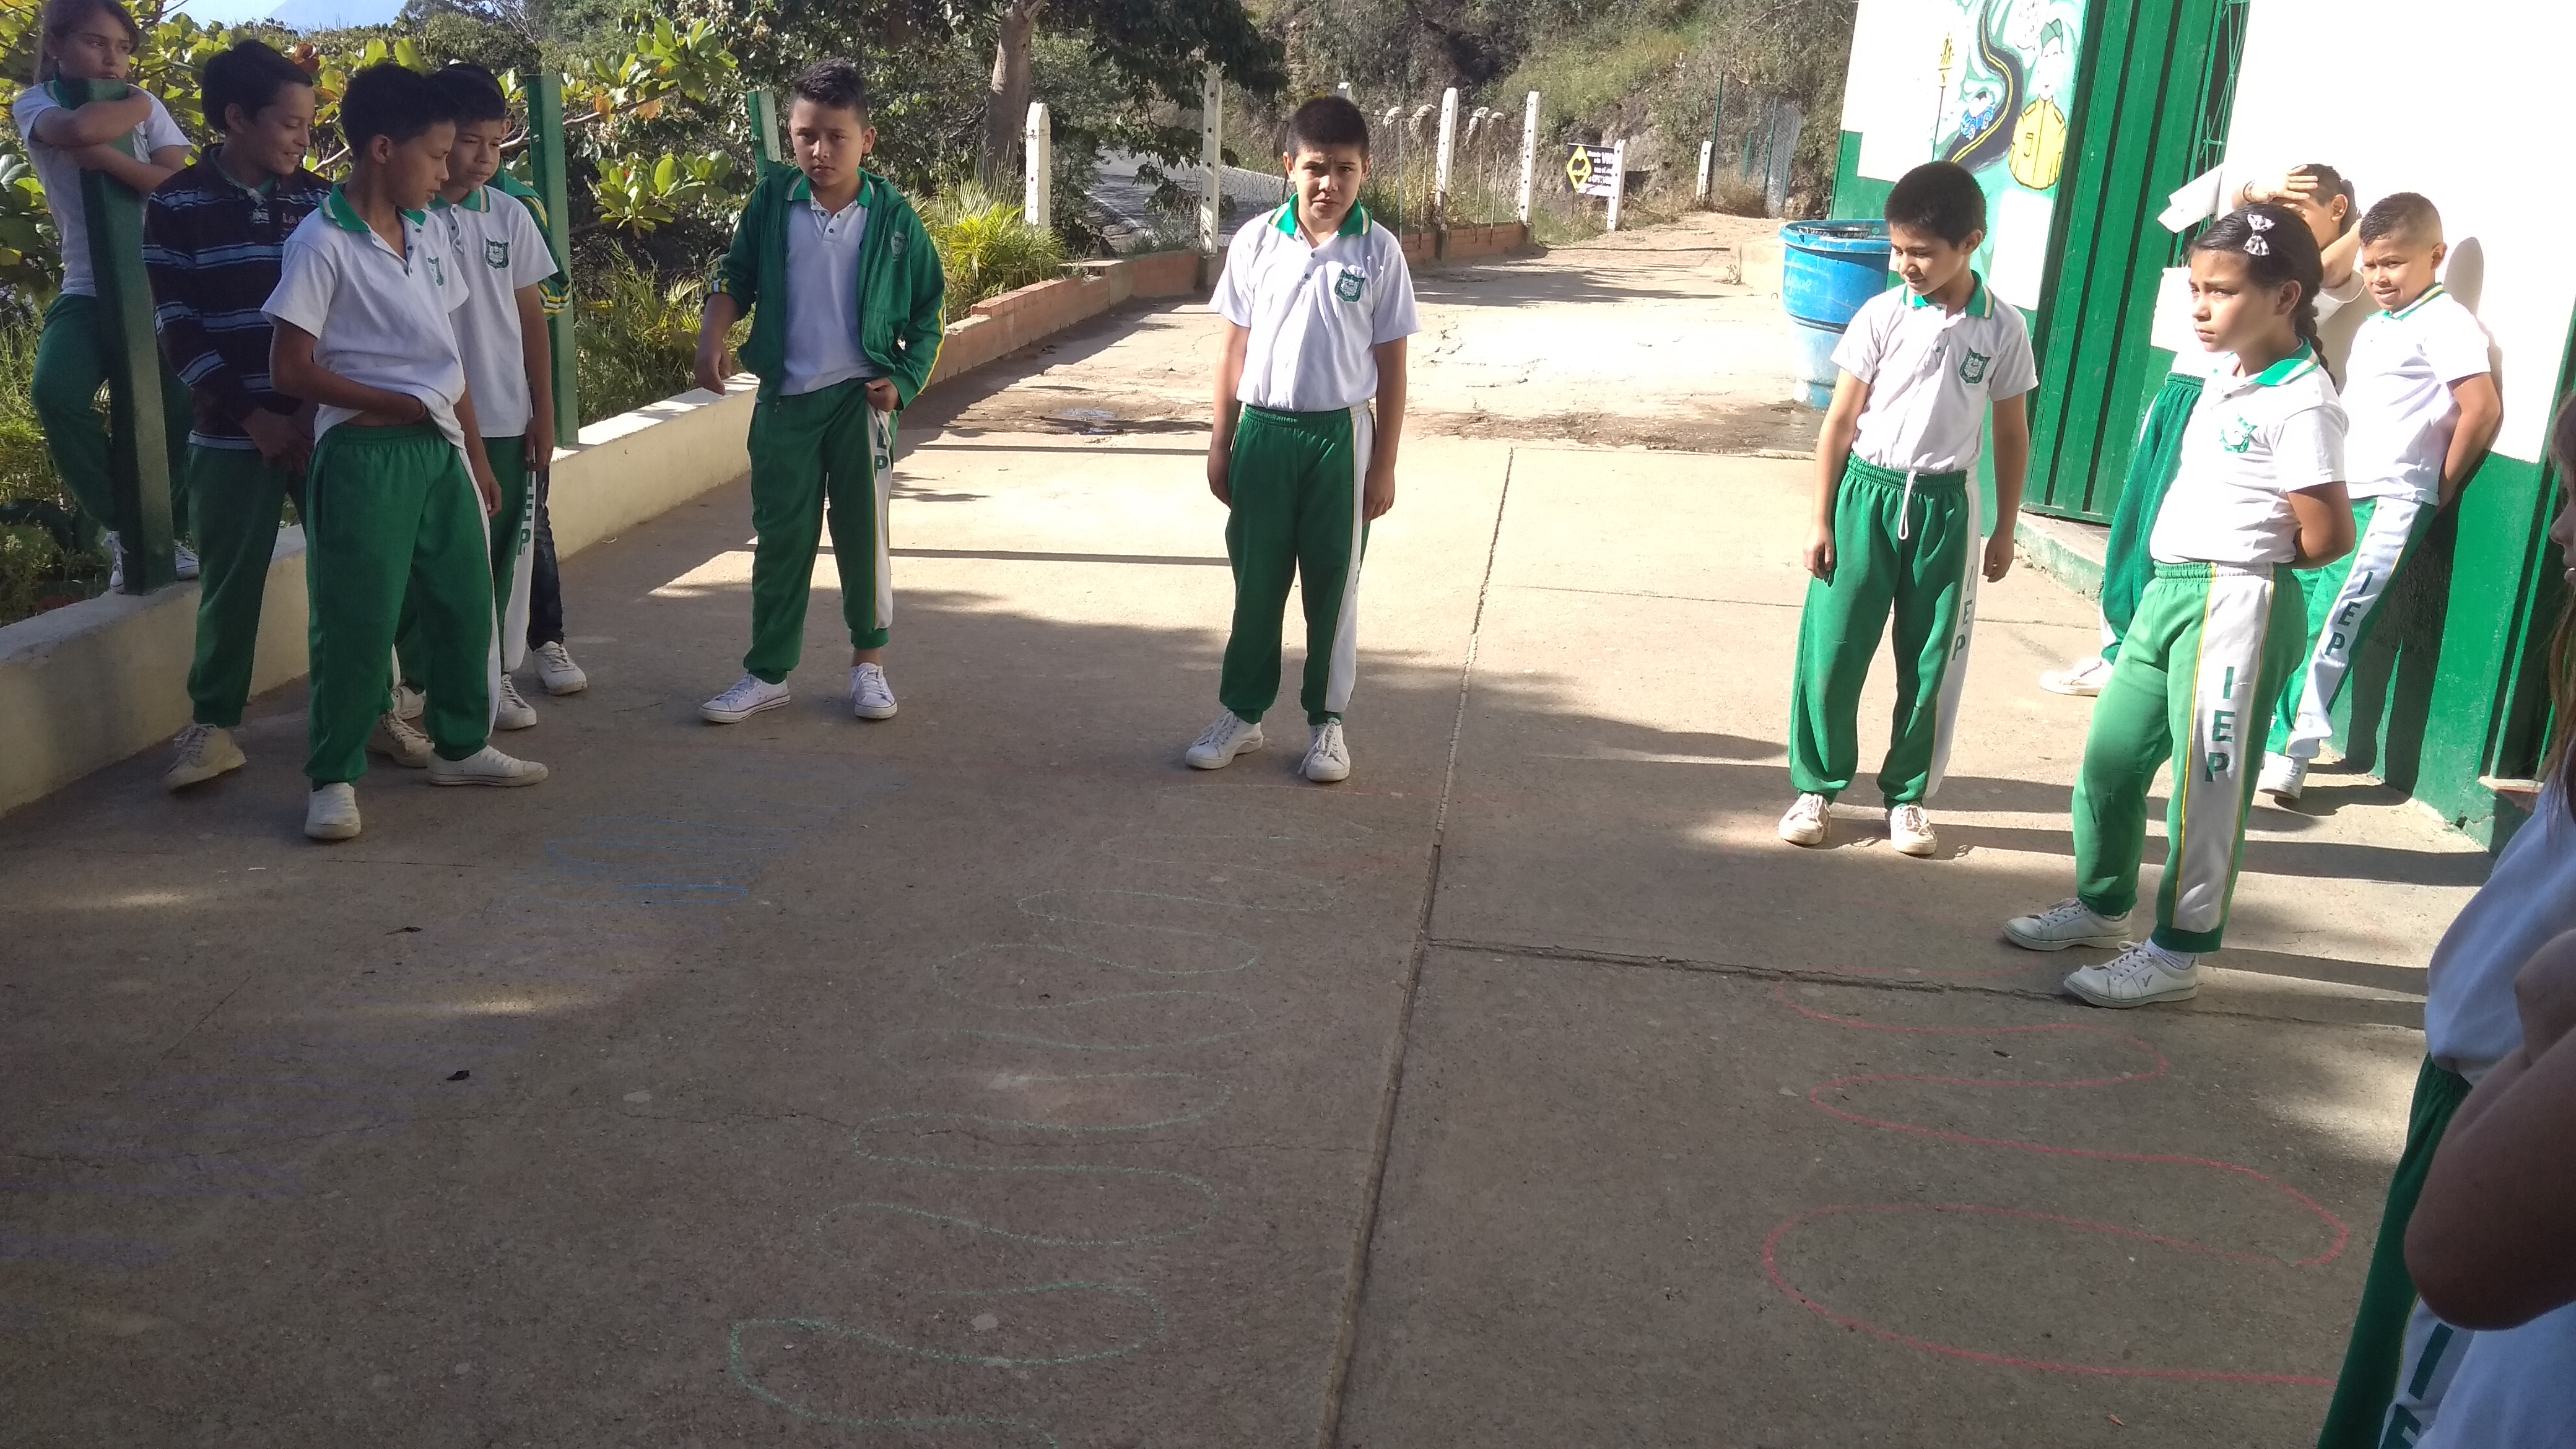
\includegraphics[width = 8.3 cm]{Imagenes/porticoonda.jpg}
    \caption{Ondas electromagnéticas con diferente frecuencia y longitud de onda realizadas en la Institución Educativa Clavellinas (superior) y en la Institución Educativa El Pórtico (inferior).}
\end{figure}

\noindent \textbf{Espectro de la luz (2 horas y 40 minutos)}\\
En esta sección se explicó el espectro de la radiación electromagnética empezando por la luz visible. En esta parte se explicó que la luz blanca está compuesta que todos los colores y para afianzar tales conocimientos se observó la descomposición de la luz por medio de un prisma y además, se realizó la construcción de un espectroscopio con un CD viejo. Este espectroscopio permite descomponer la luz blanca de los bombillos y/o fluorescentes en todos los colores del espectro visible y además, permite medir la longitud de onda de cada una de las componentes.

\begin{figure}[H]
    \centering
    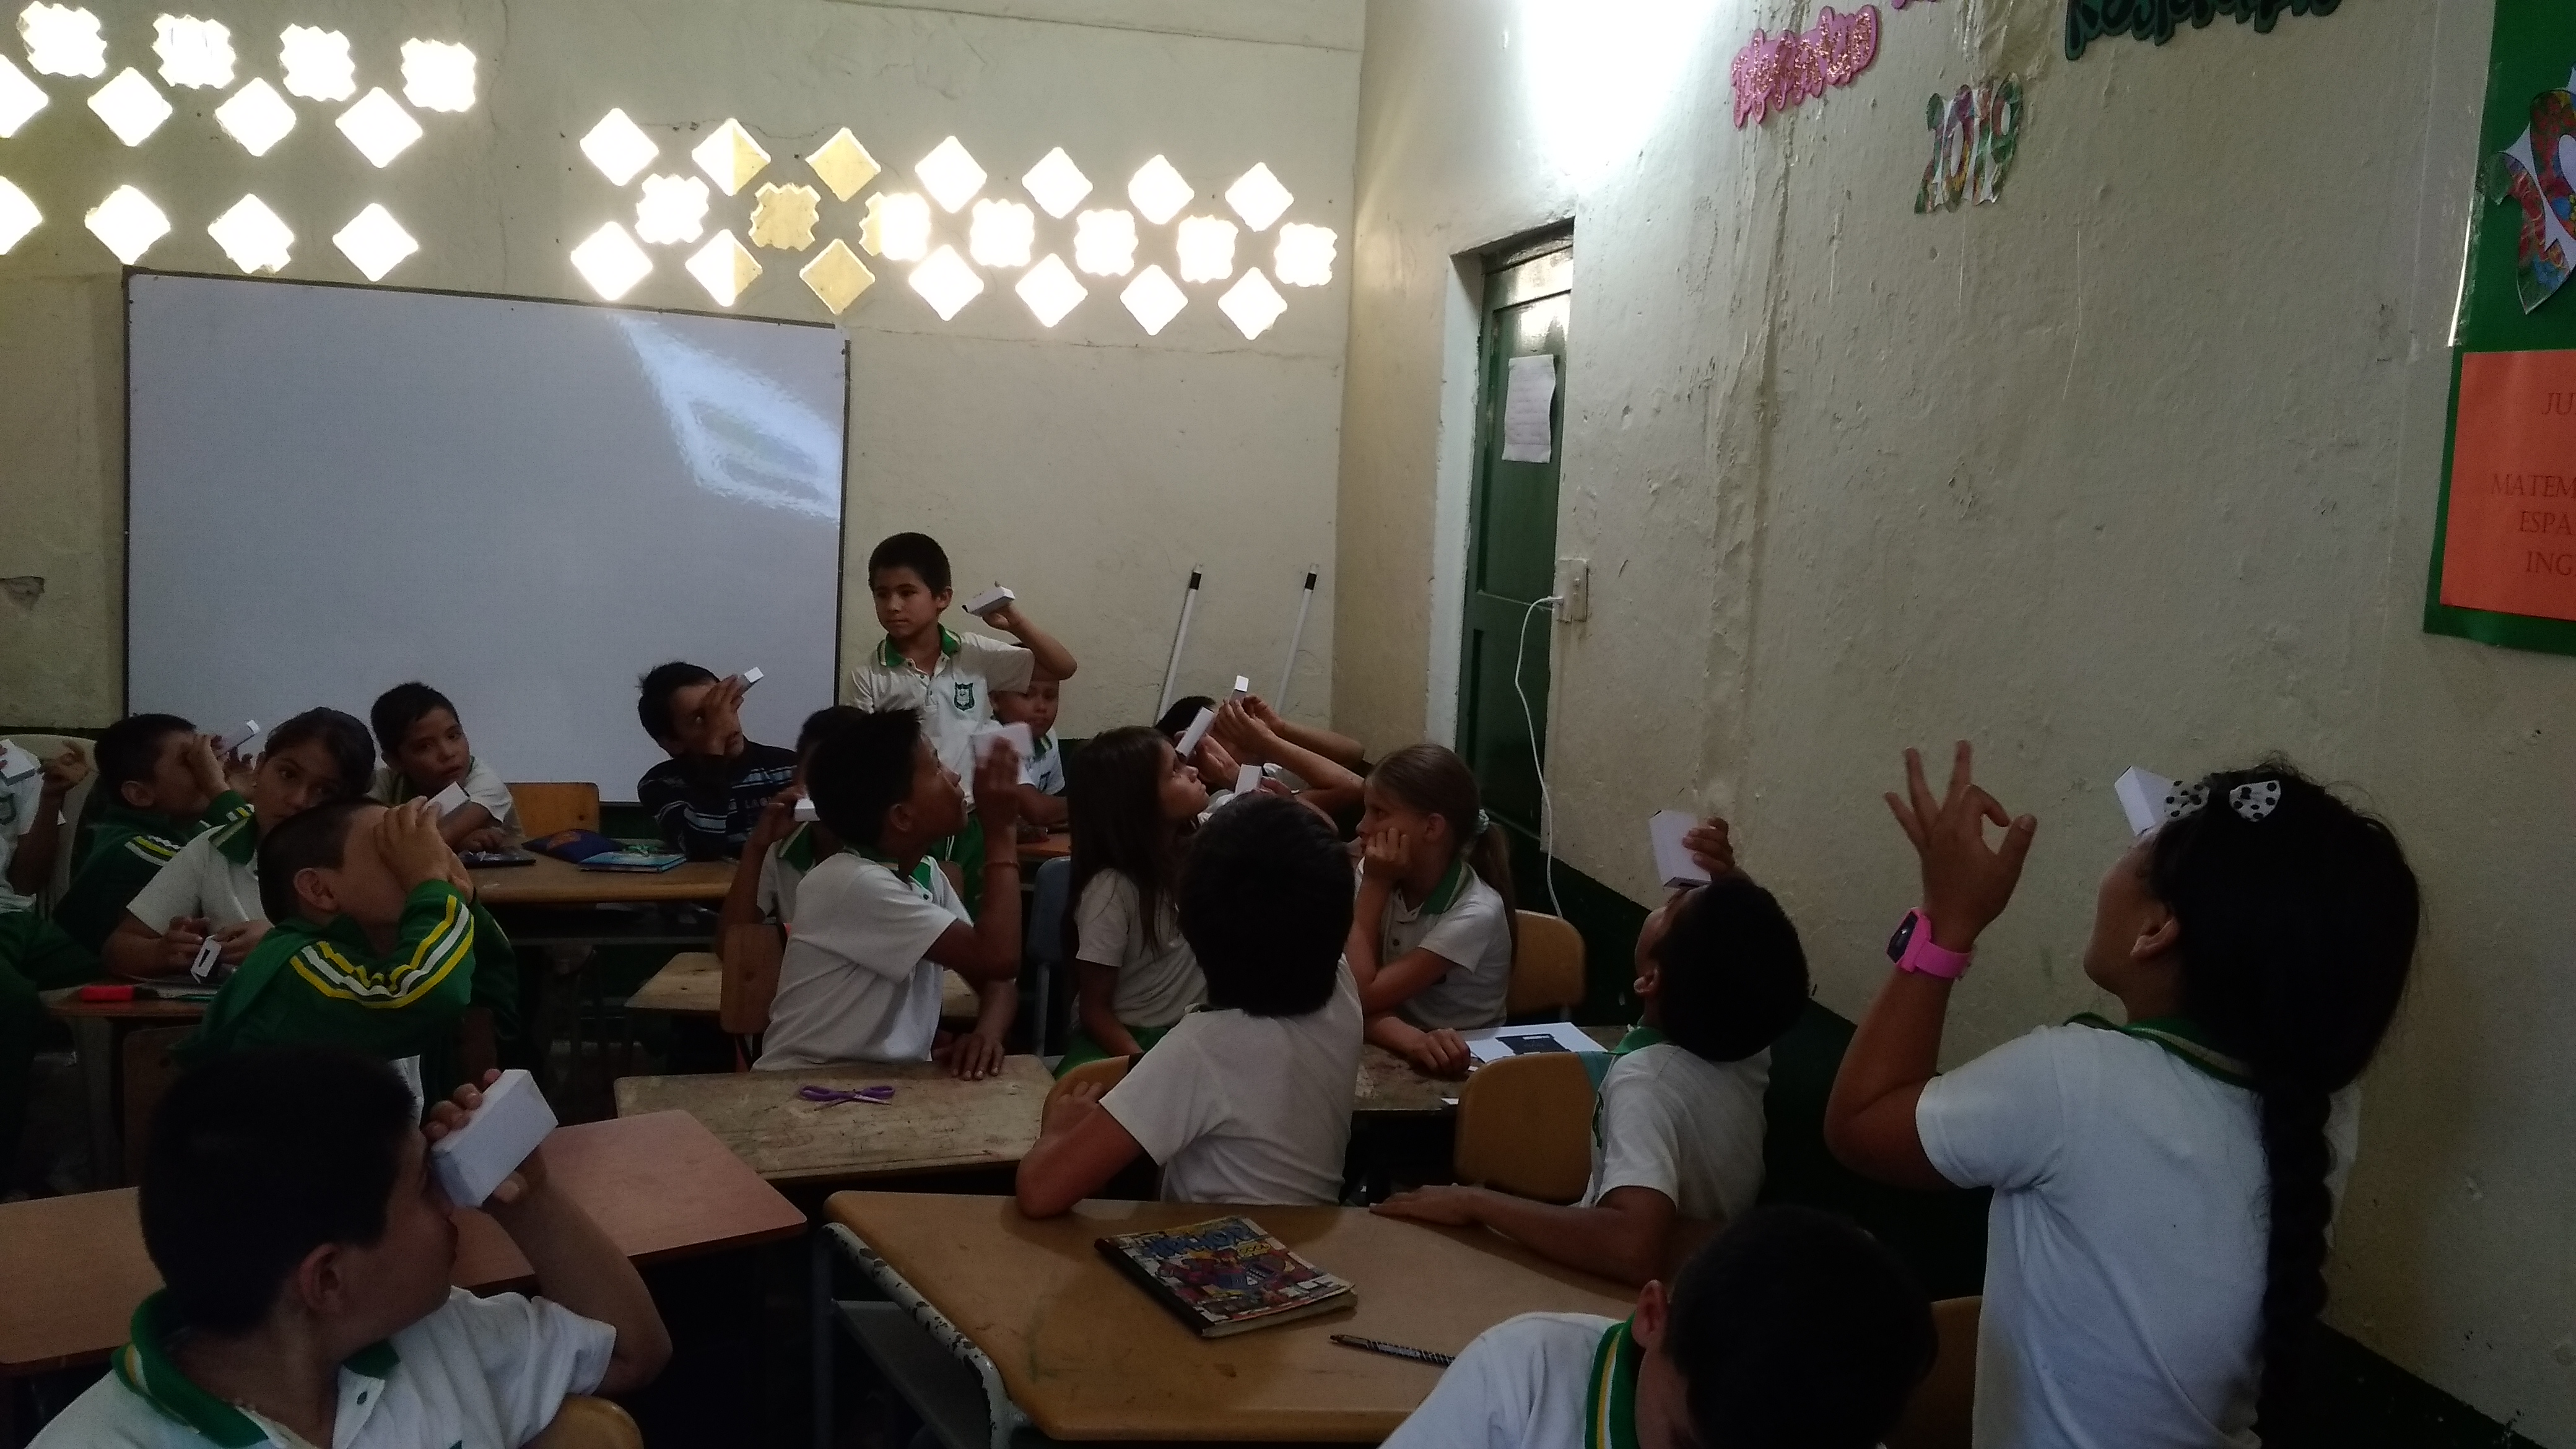
\includegraphics[width = 8.2 cm]{Imagenes/espectroportico.jpg}
    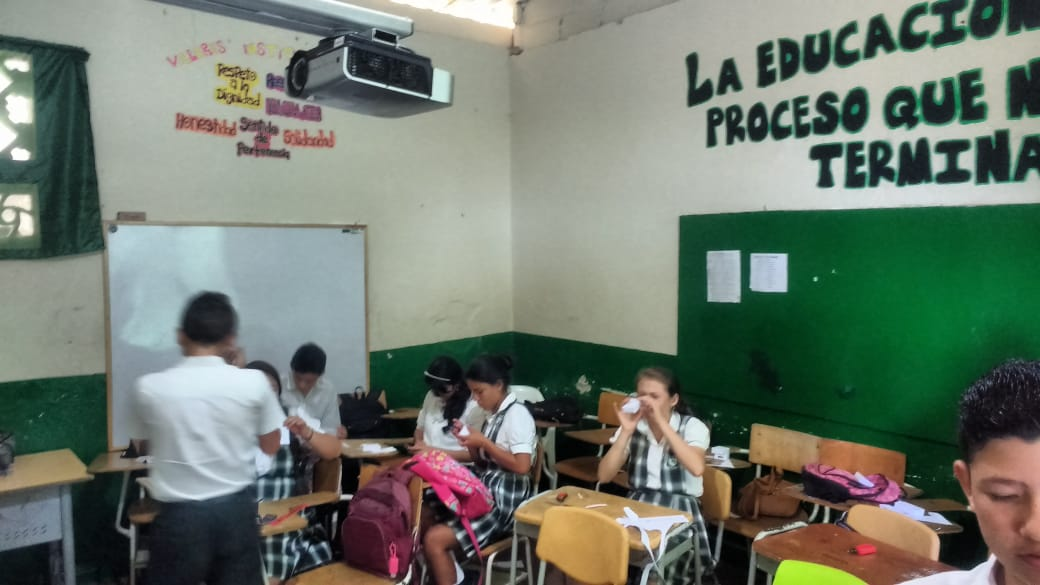
\includegraphics[width = 8.2 cm]{Imagenes/luz1}
    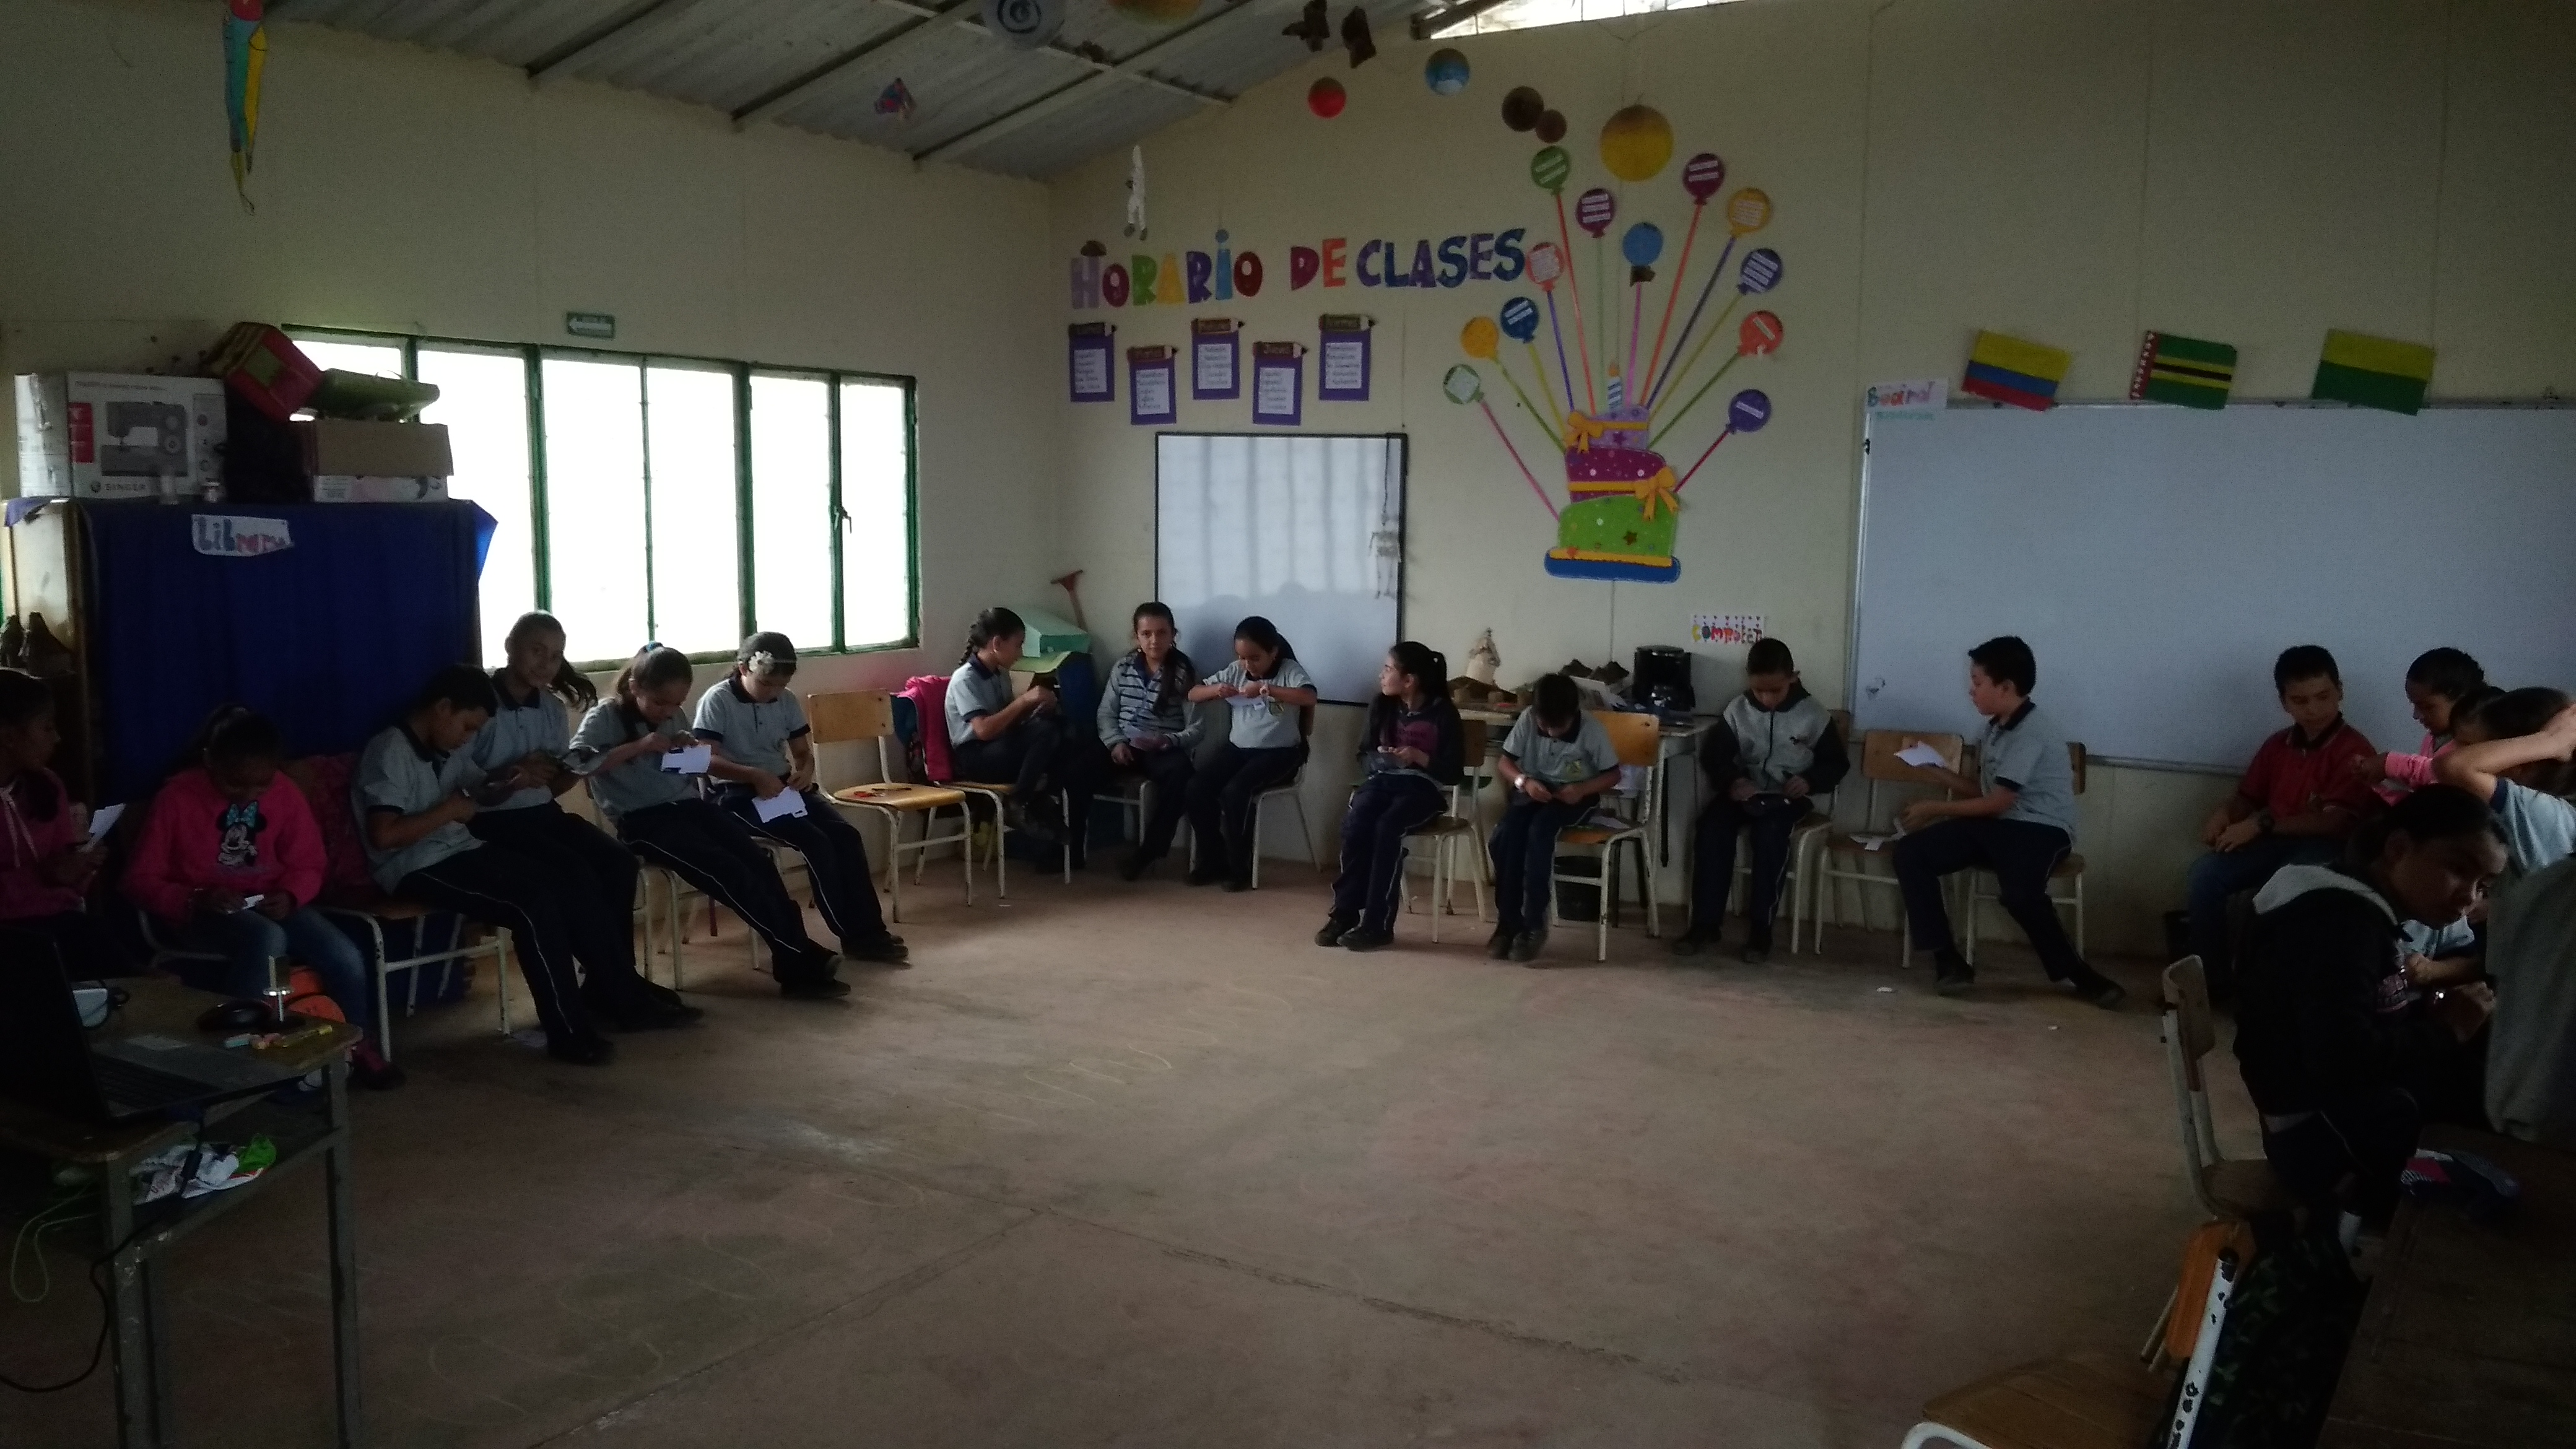
\includegraphics[width = 8.2 cm]{Imagenes/espectroclave.jpg}
    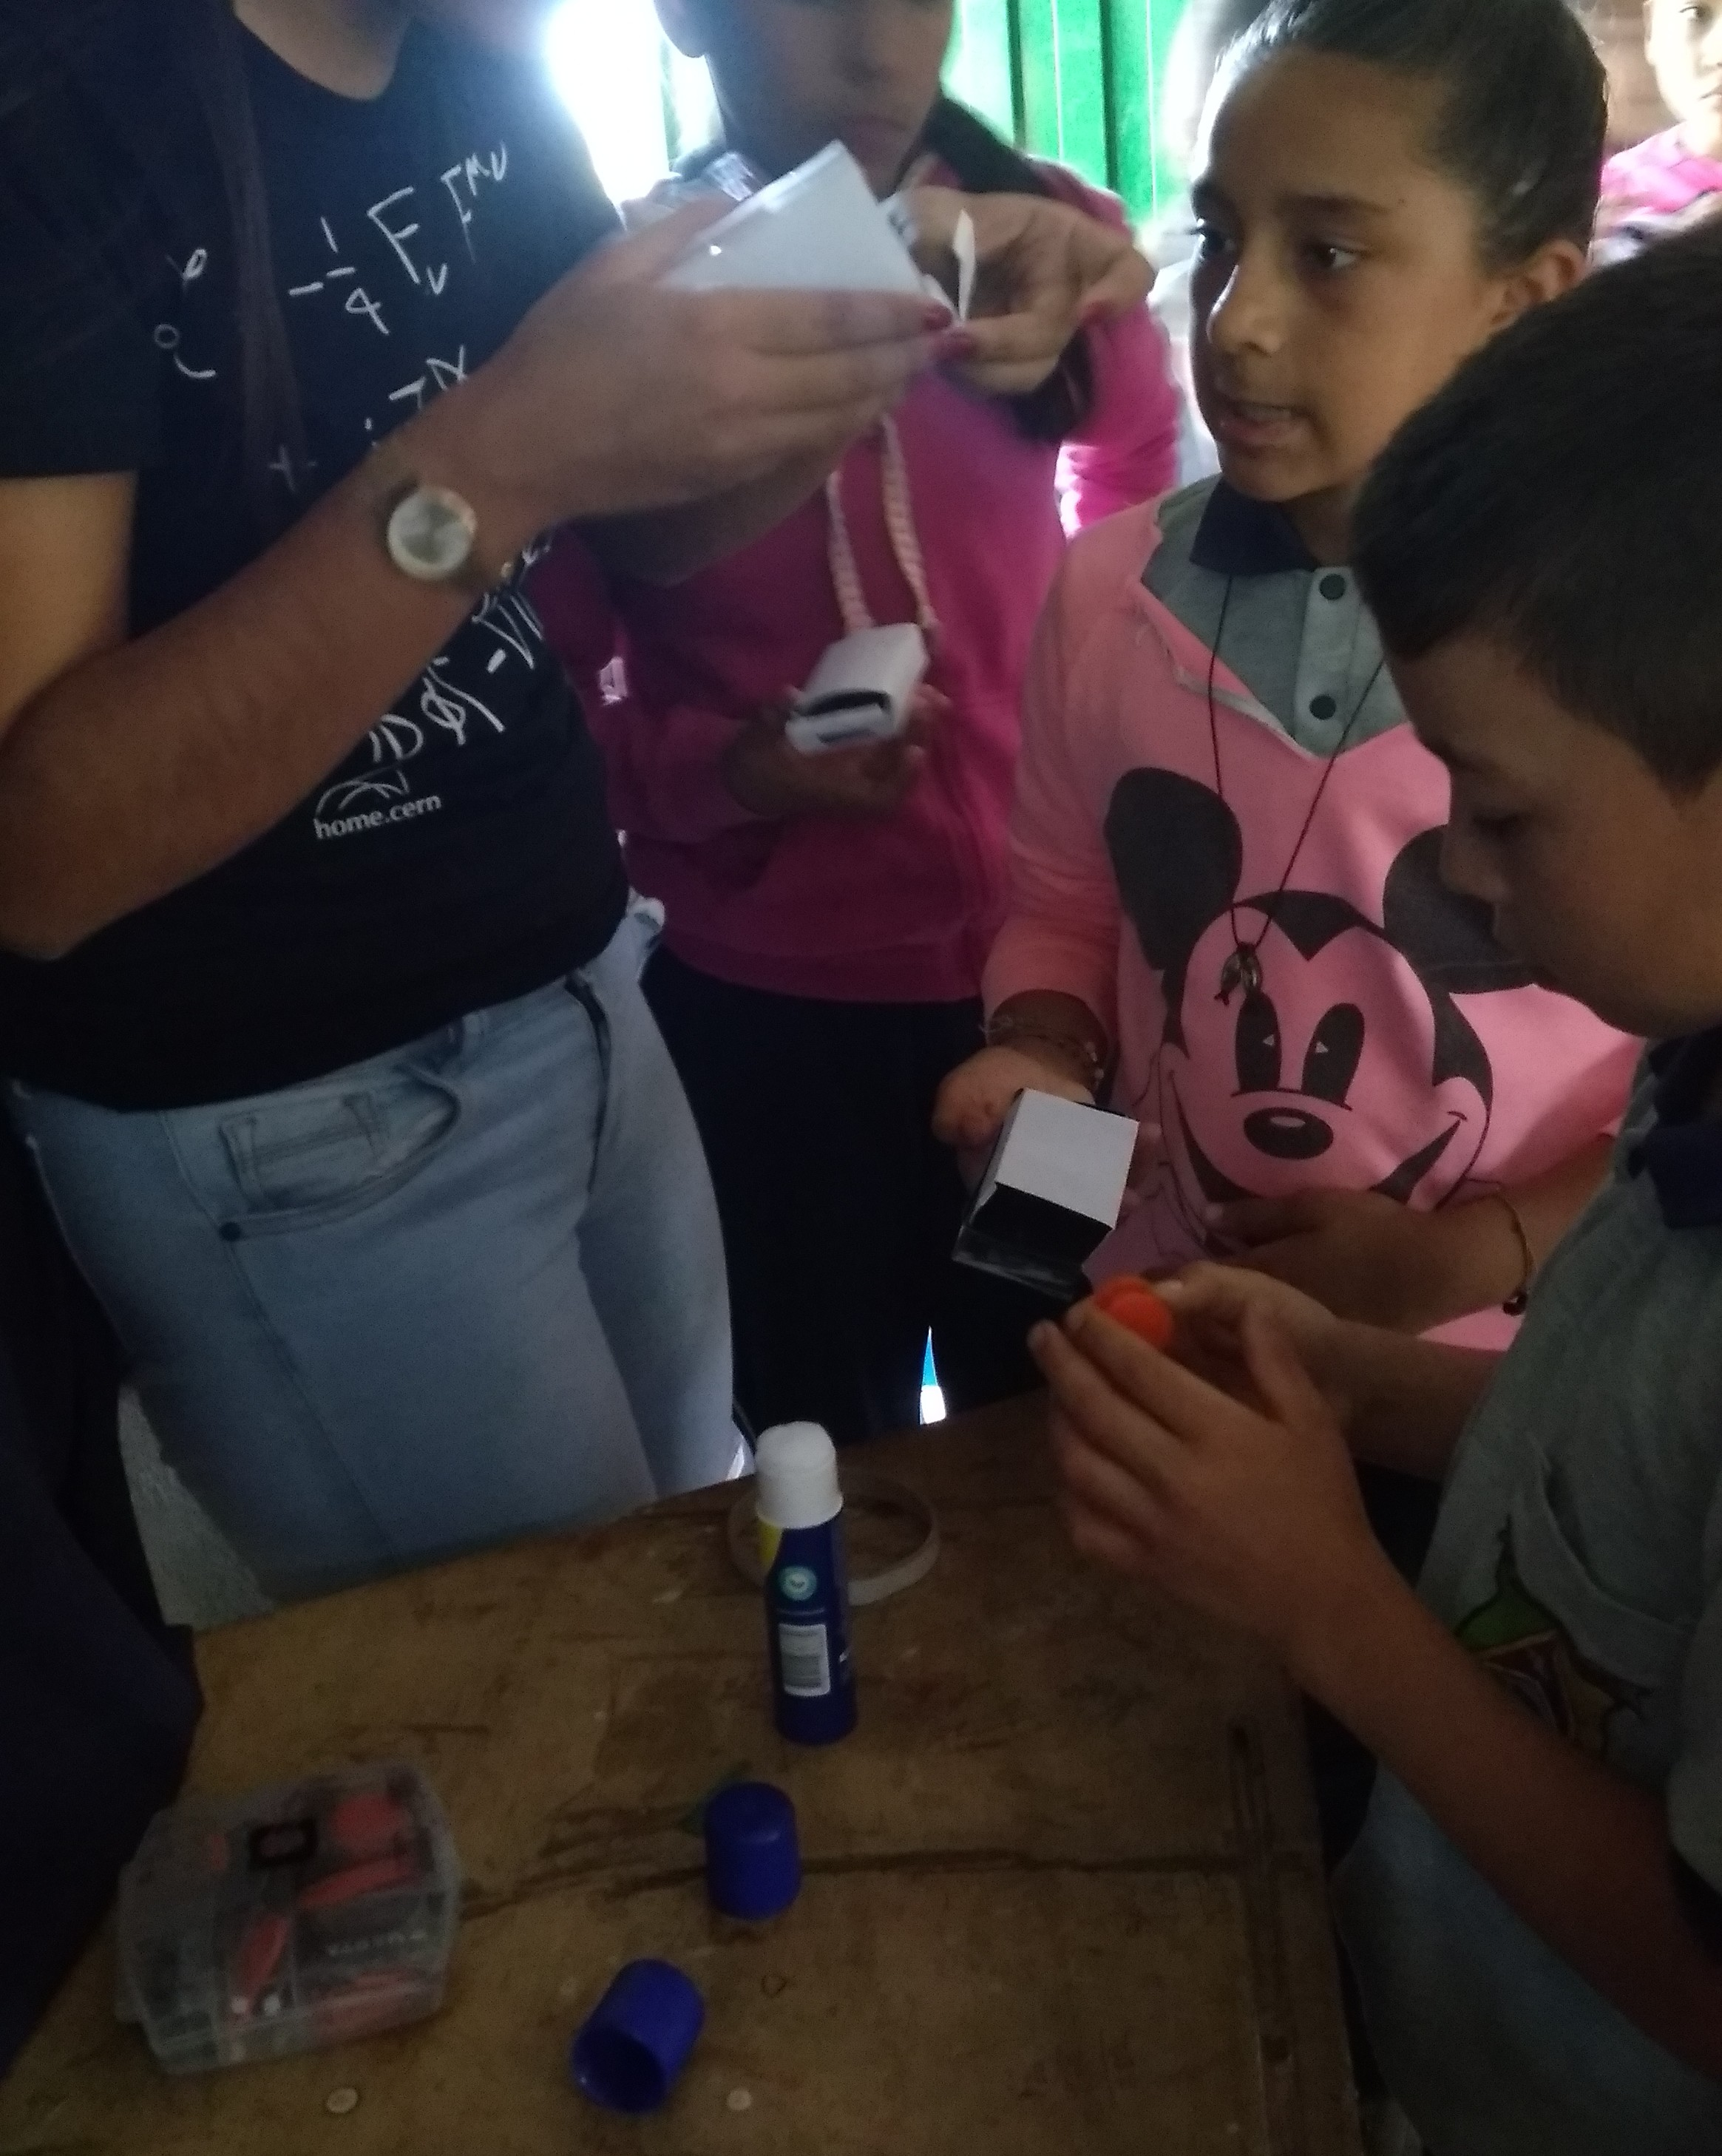
\includegraphics[width = 3.7 cm]{Imagenes/pegarclave.jpg}
    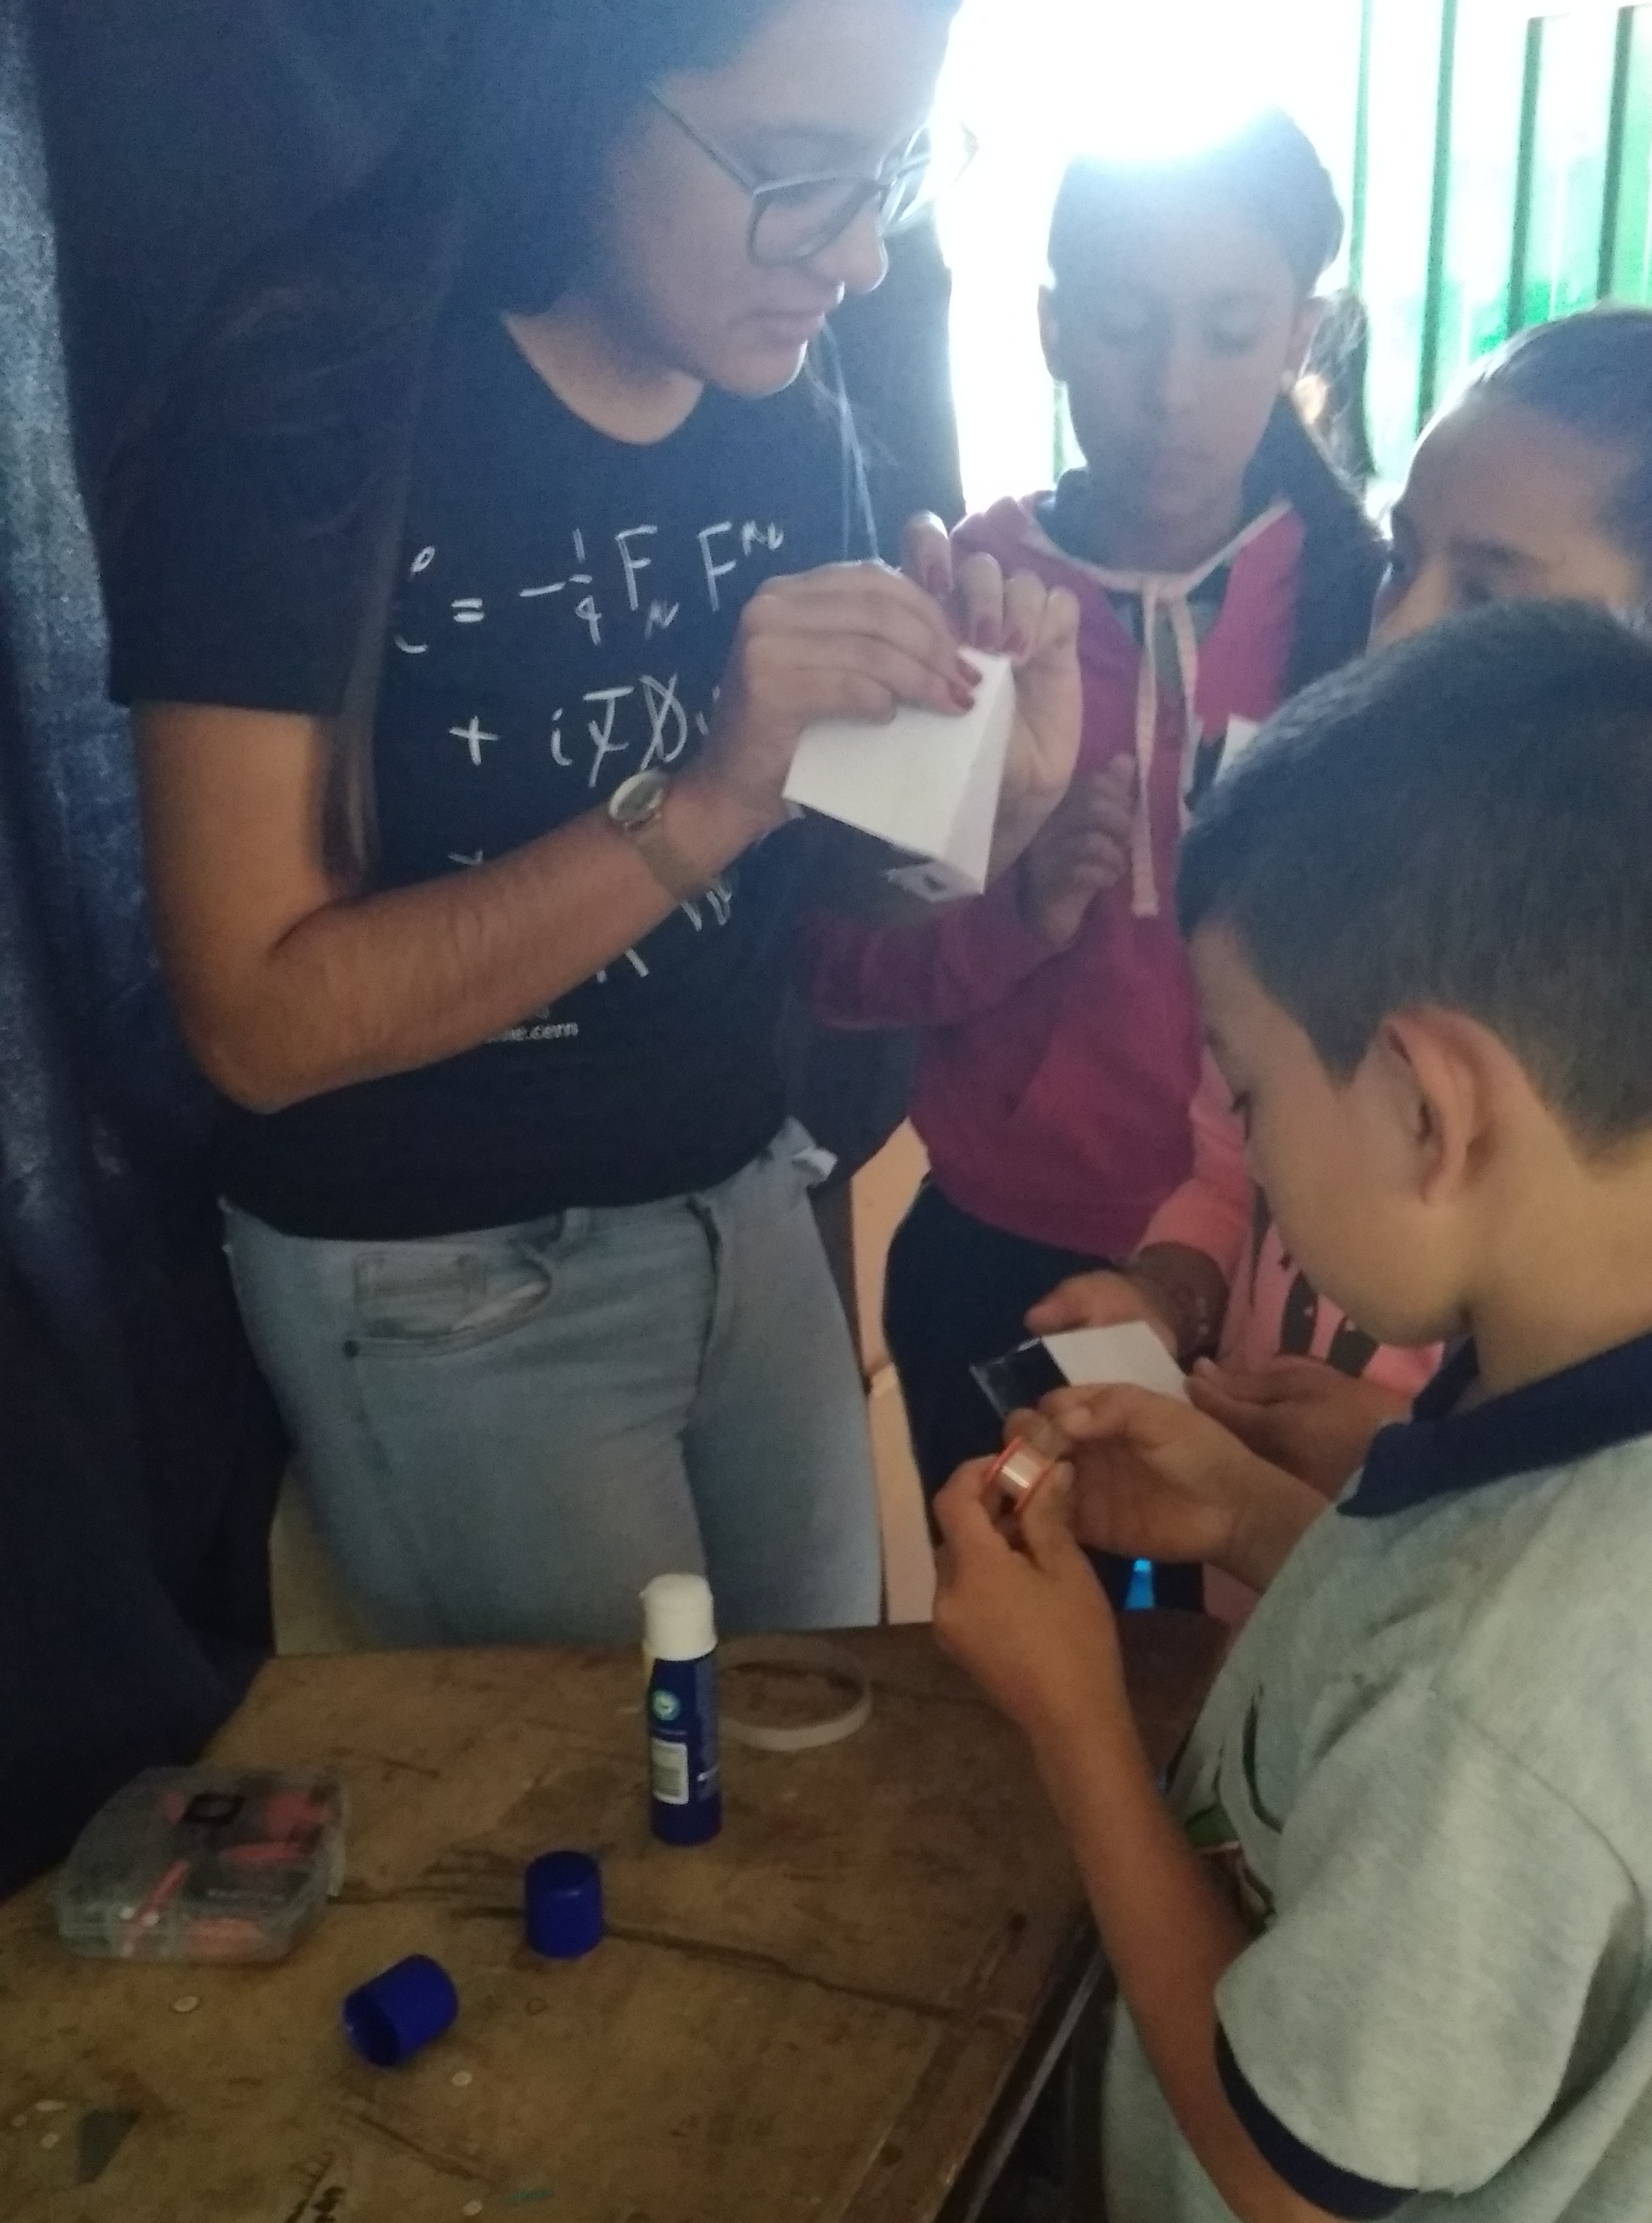
\includegraphics[width = 3.45 cm]{Imagenes/espectrolaura.jpg}
    \caption{Construcción del espectroscópio en las Instituciones Educativas El Pórtico (superior) y Clavellinas (inferior).}
\end{figure}
\noindent Una vez finalizado el proceso de construcción del espectroscopio, los chicos lo usaron para observar la luz de los bombillos, del vídeo-beam y algunos haces de la luz del sol. Luego, se discutió acerca del tipo de espectro que observaron y si este era continuo o eran líneas separadas.
\begin{figure}[H]
    \centering
    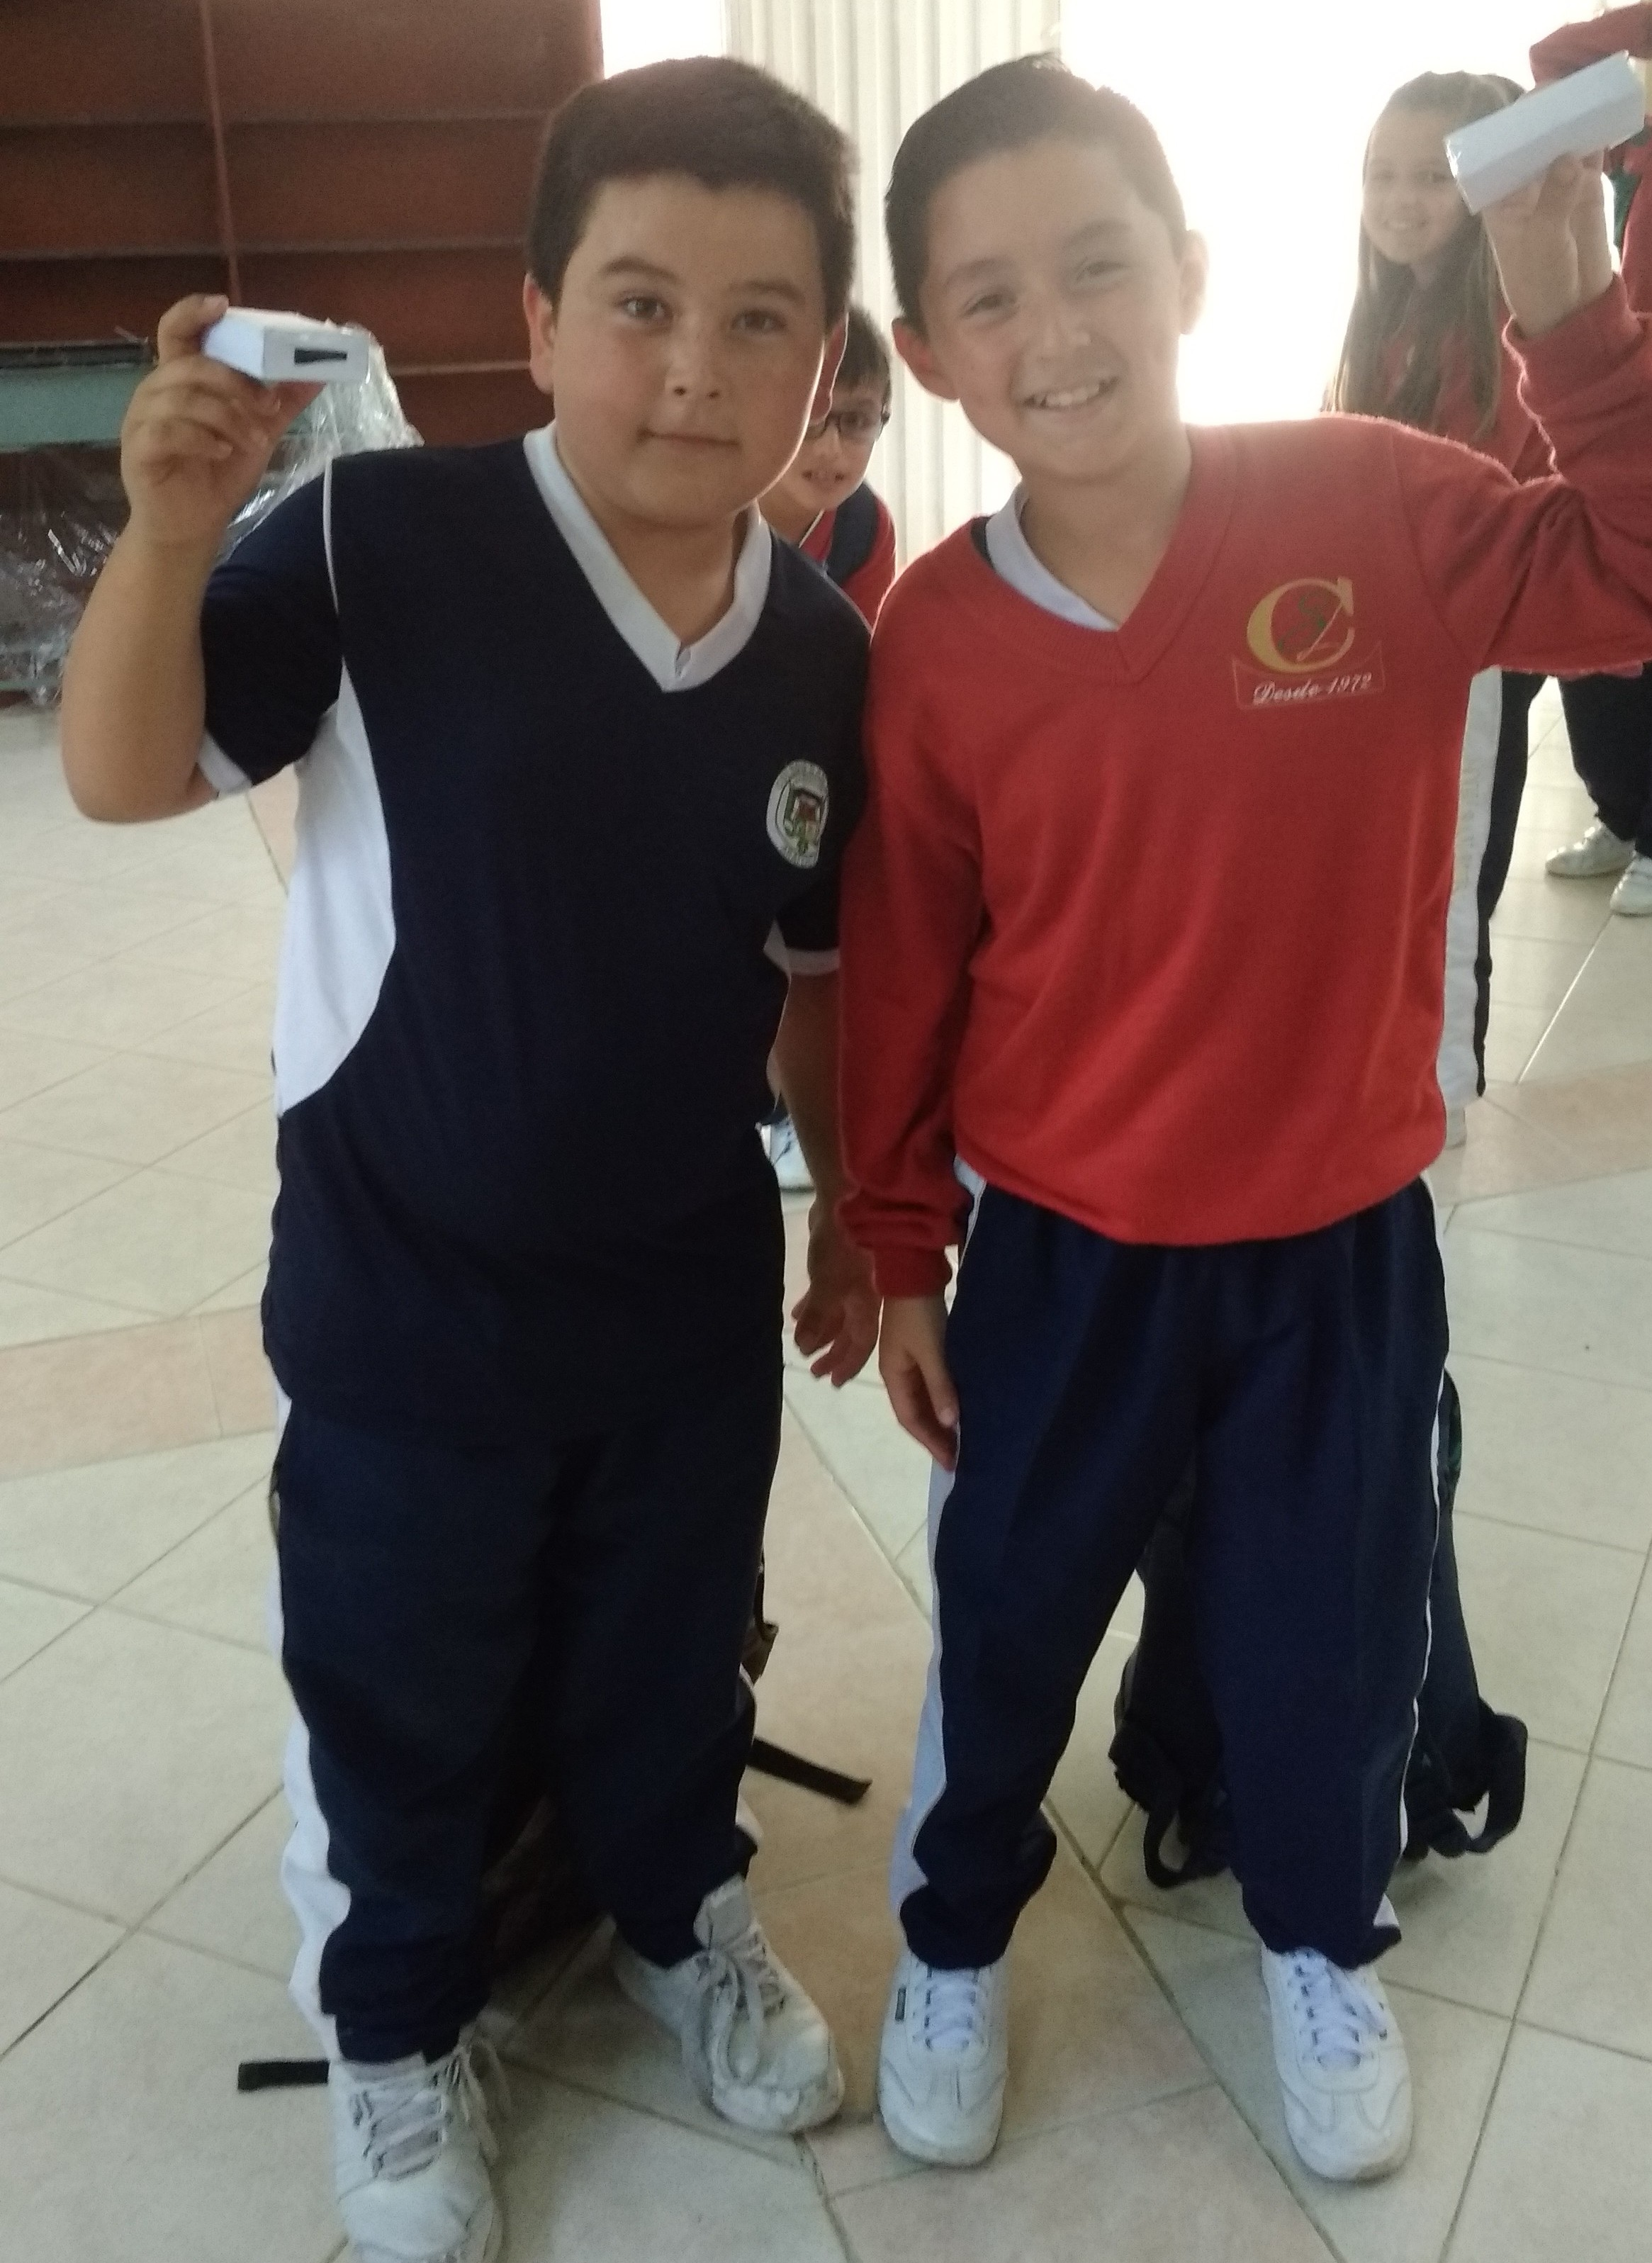
\includegraphics[width = 5.0 cm]{Imagenes/espectrosanluis.jpg}
    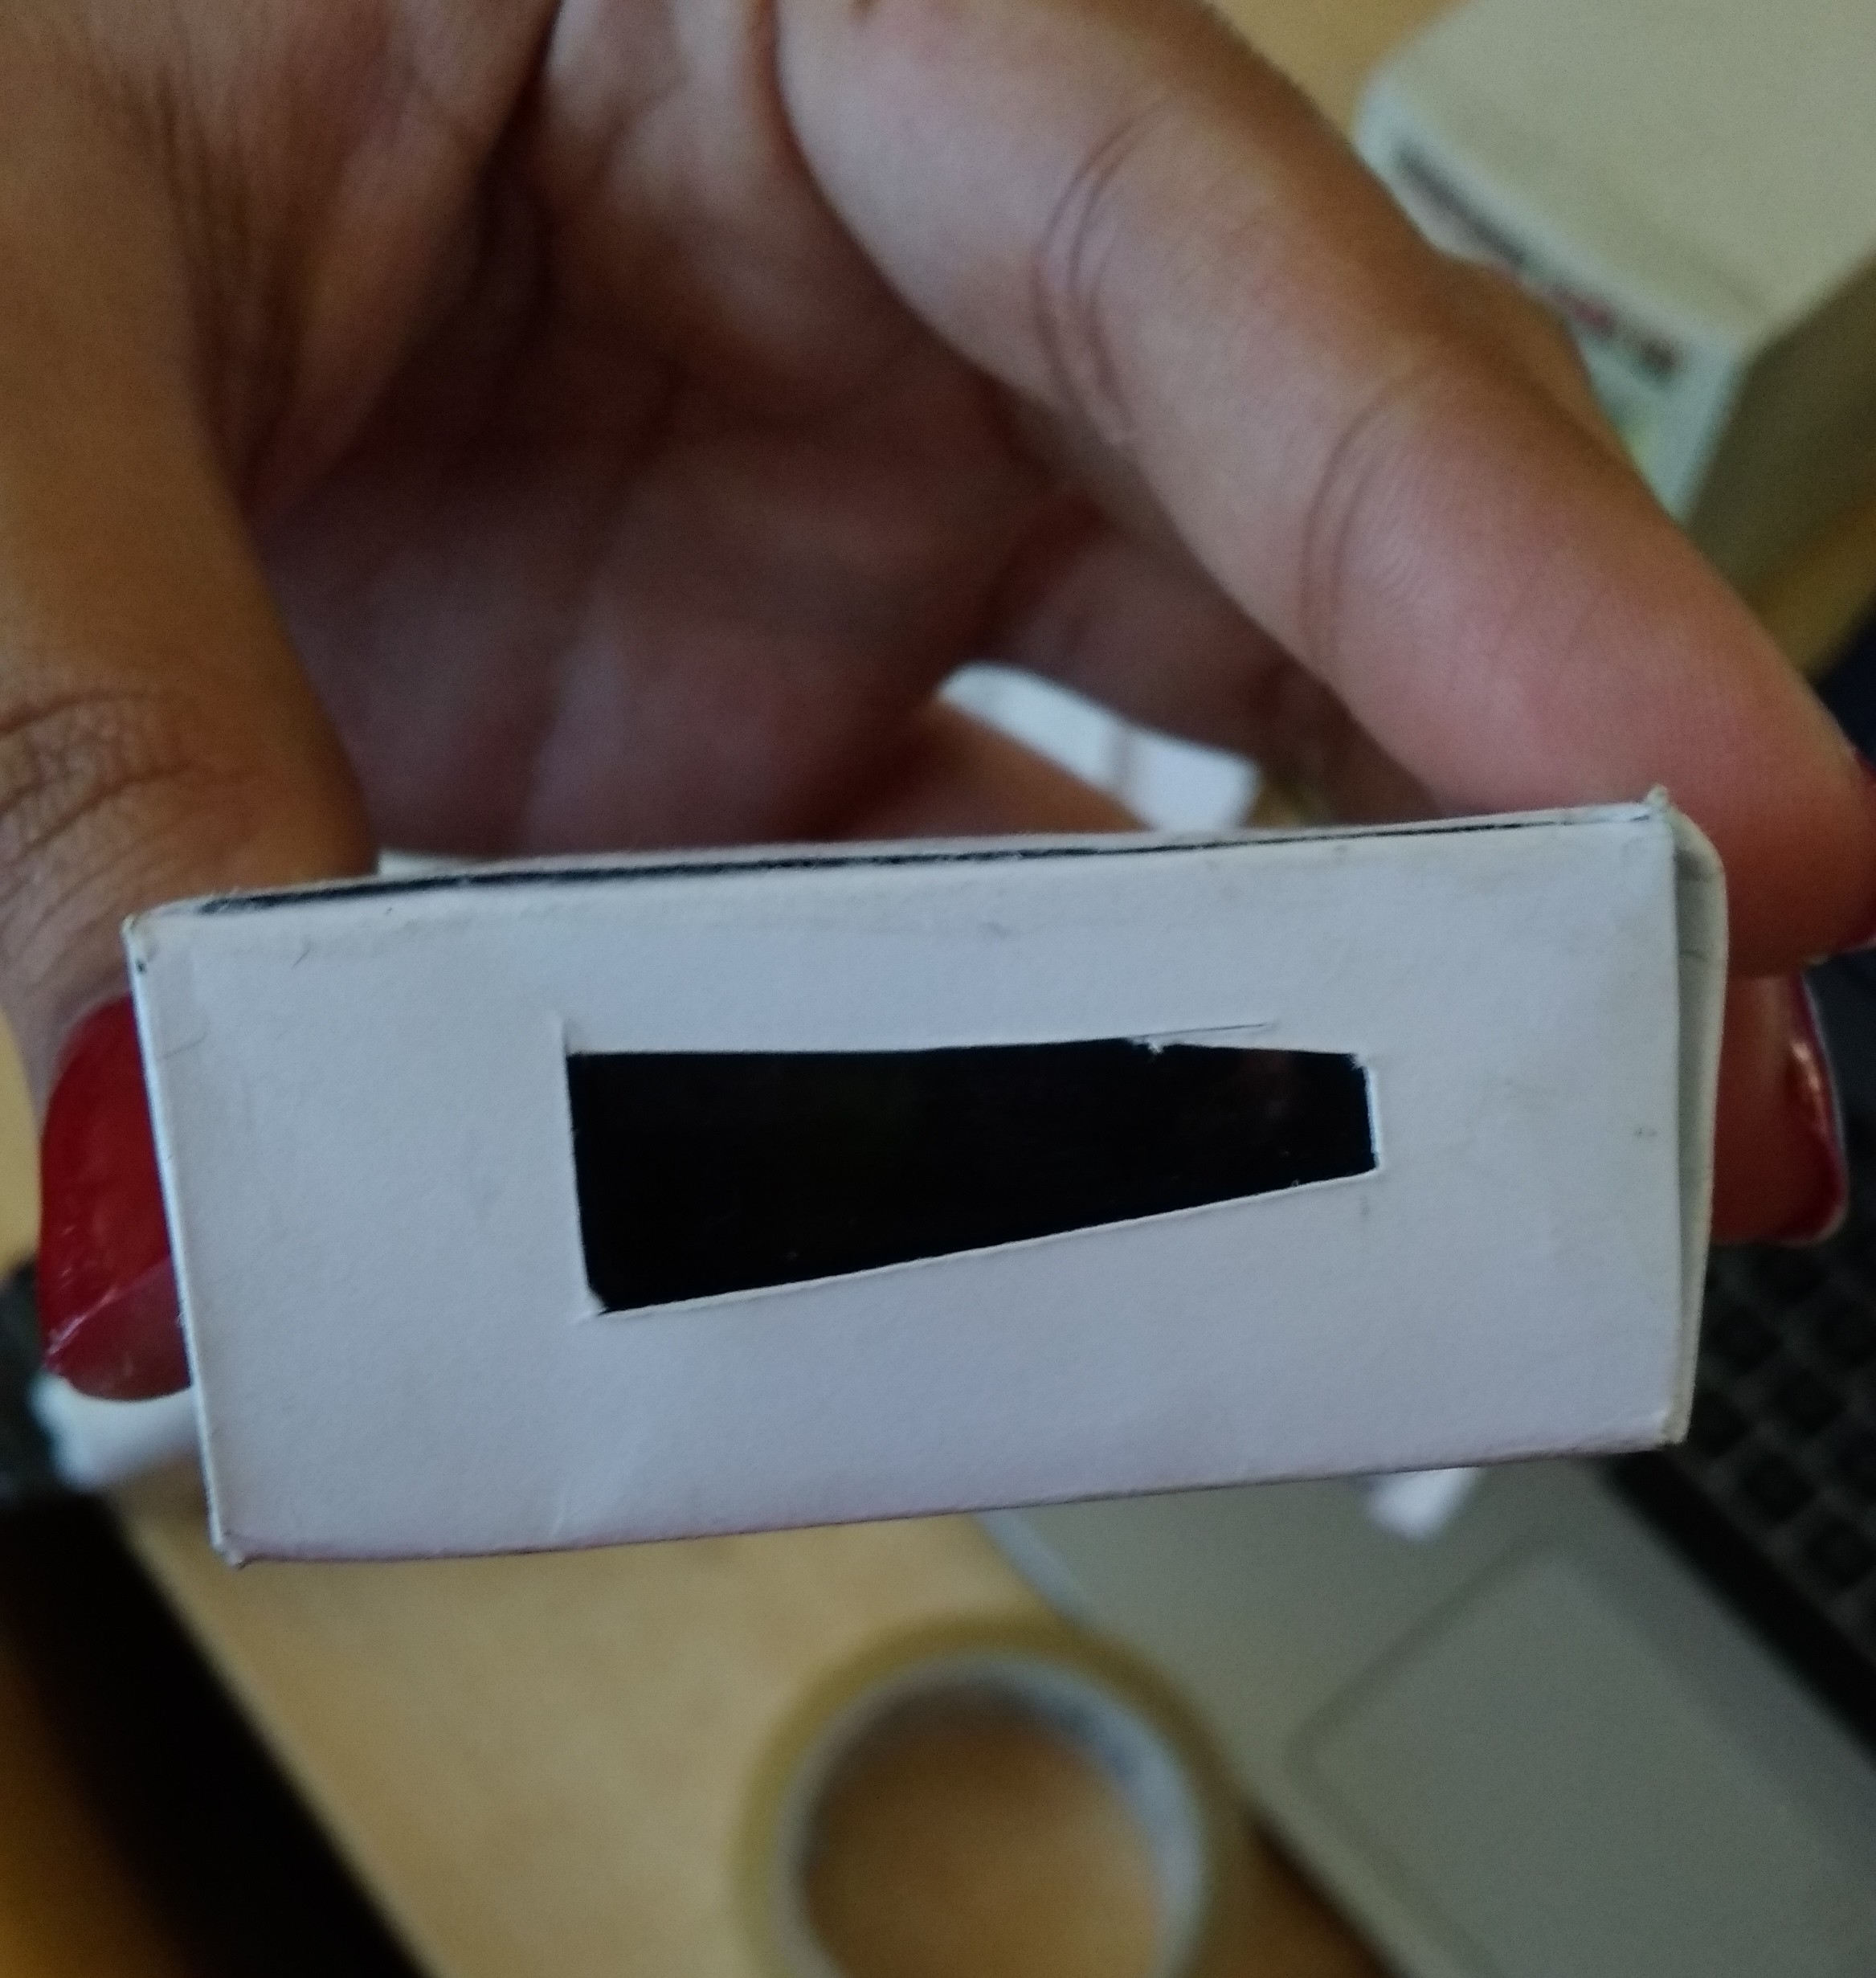
\includegraphics[width = 6.5 cm]{Imagenes/espectro.jpg}
    \caption{Resultado final del proceso de construcción del espectroscopio en el Colegio San Luis (izquierda) y en la Institución Educativa El Pórtico (derecha).}
\end{figure}
\noindent Se explicó que, además de poder descomponer la luz en los colores primarios, es posible realizar el proceso inverso, es decir, reconstruir el color blanco a partir de los colores primarios. Para esta actividad se hizo uso de 3 láser de colores azul, verde y rojo y se hizo enfásis en que si bien normalmente se enseña que los colores primarios son amarillo, azul y rojo; estos colores primarios solo funcionan con las pinturas, los crayones y algunos materiales; pero en óptica los verdaderos colores primarios son verde, azul y rojo.

\begin{figure}[H]
    \centering
    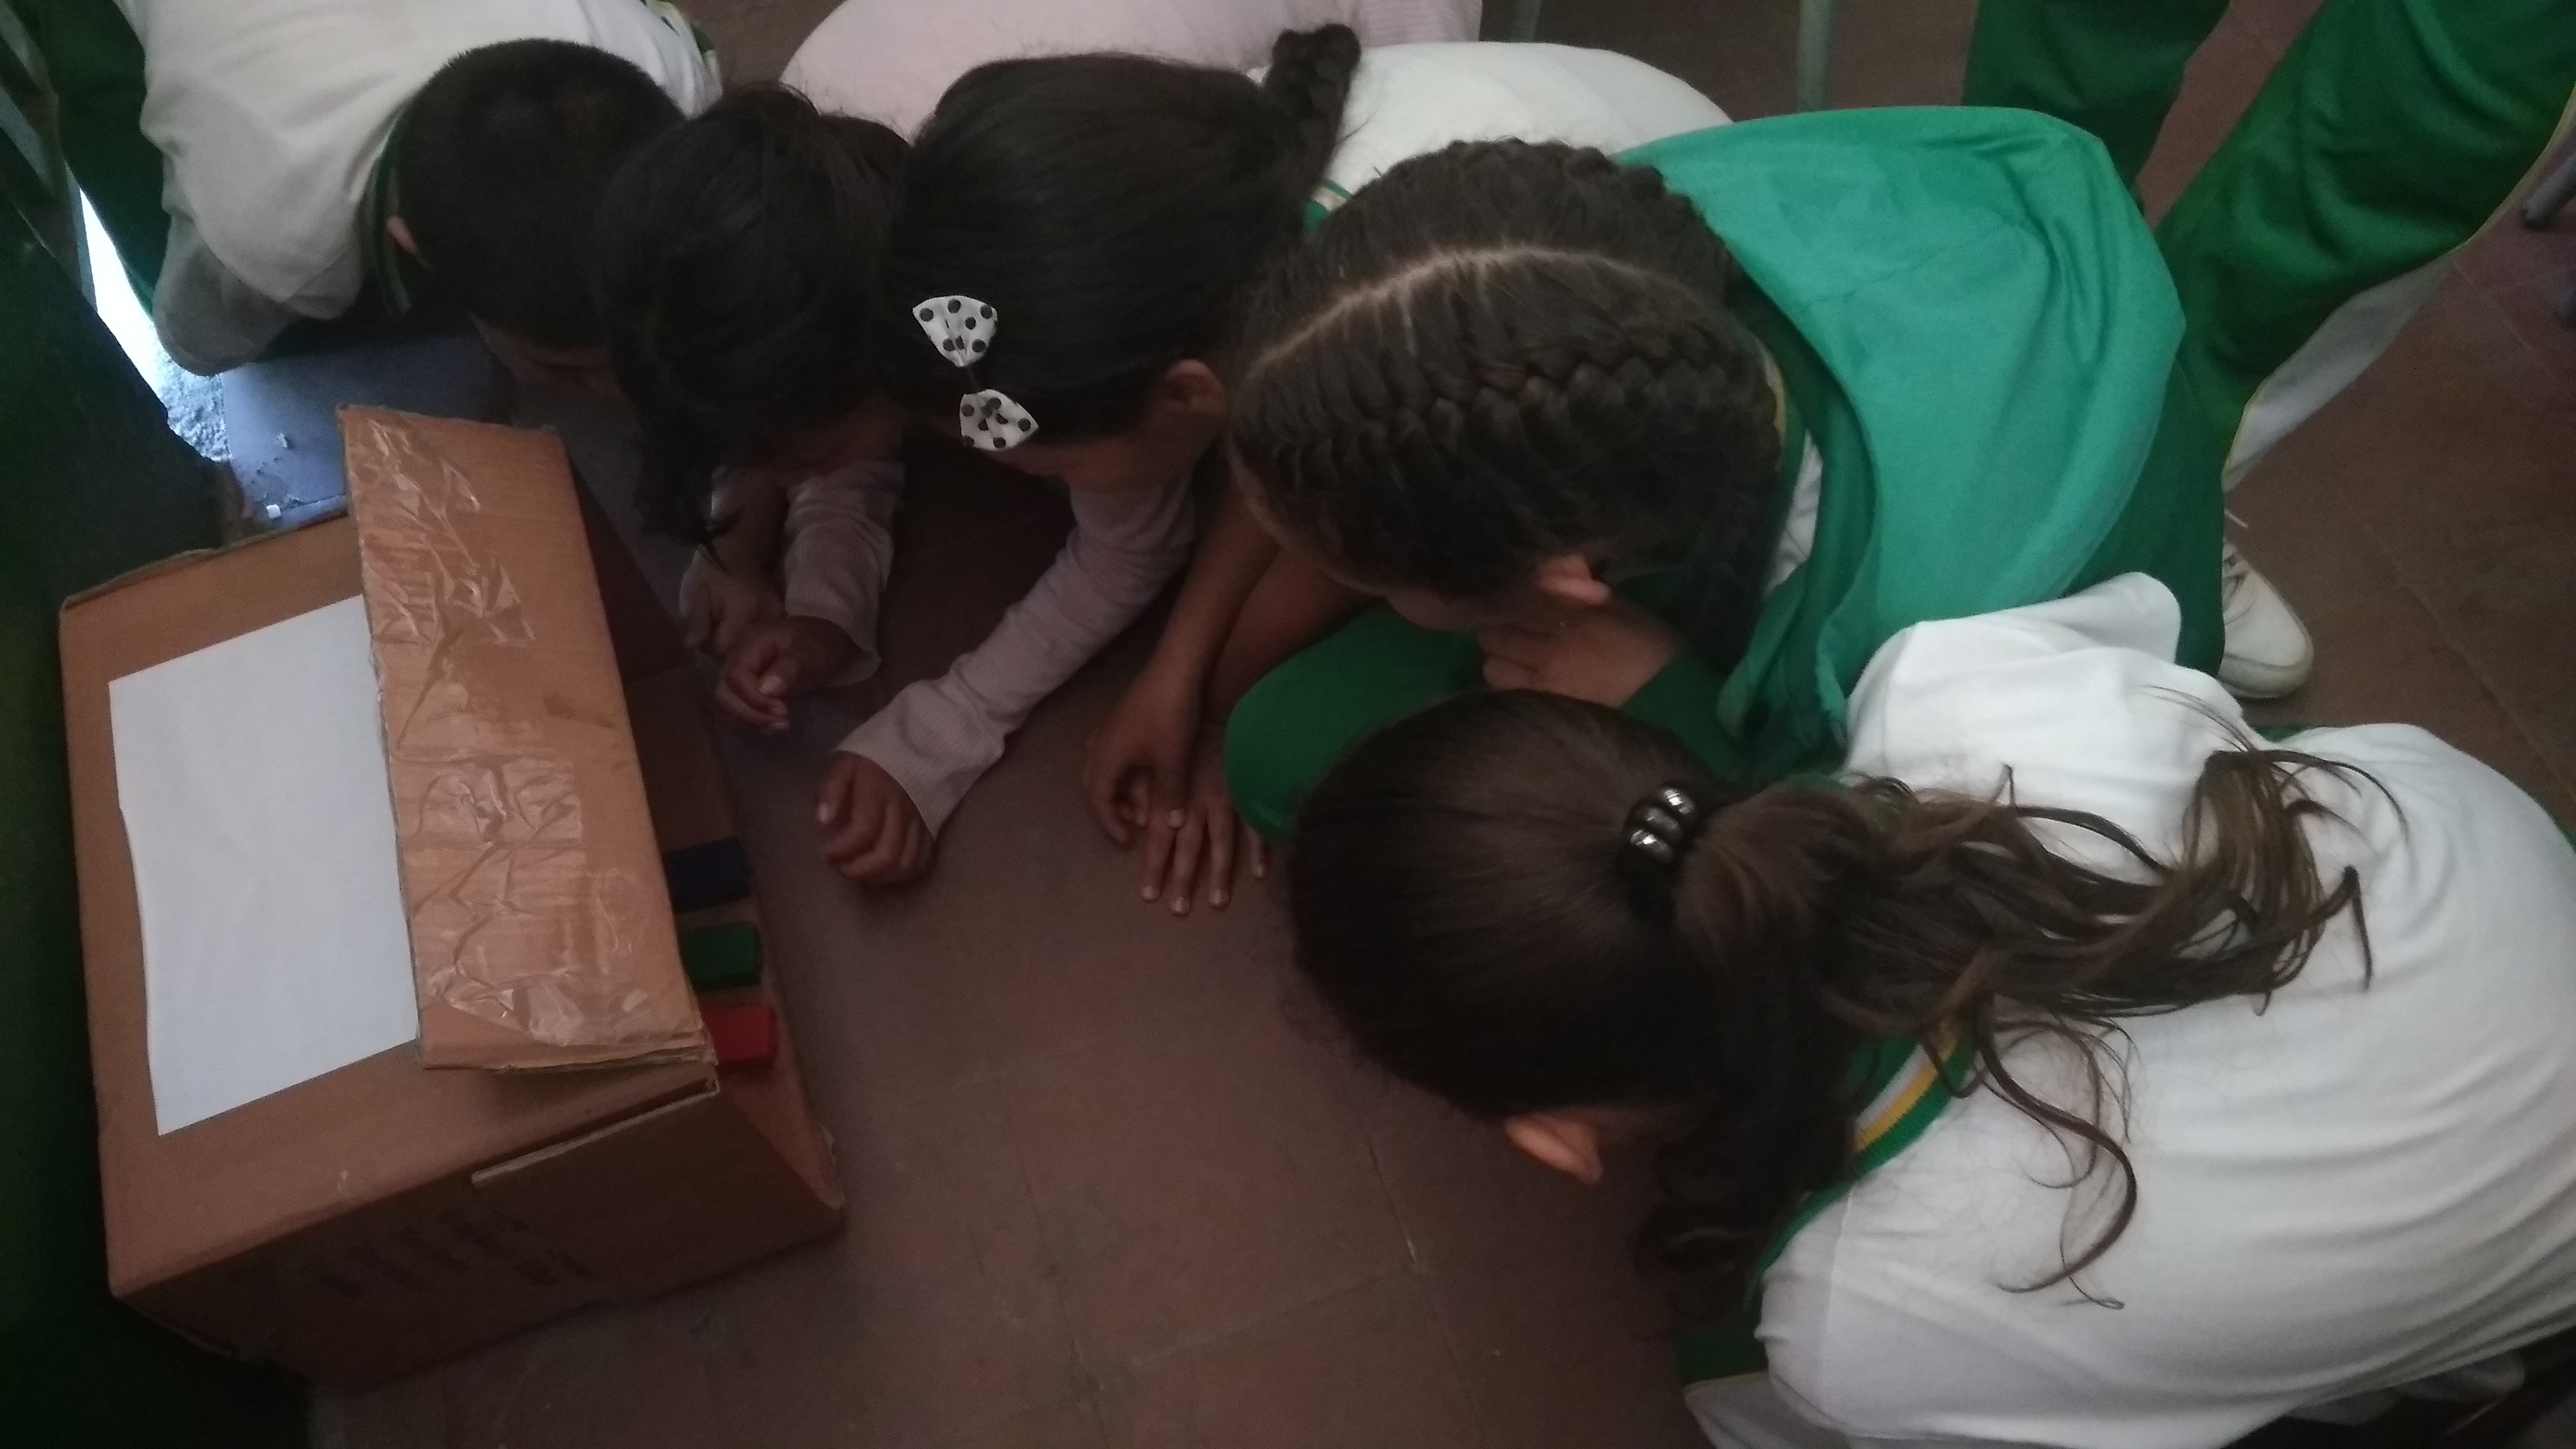
\includegraphics[width = 8.8 cm]{Imagenes/laseresportico.jpg}
    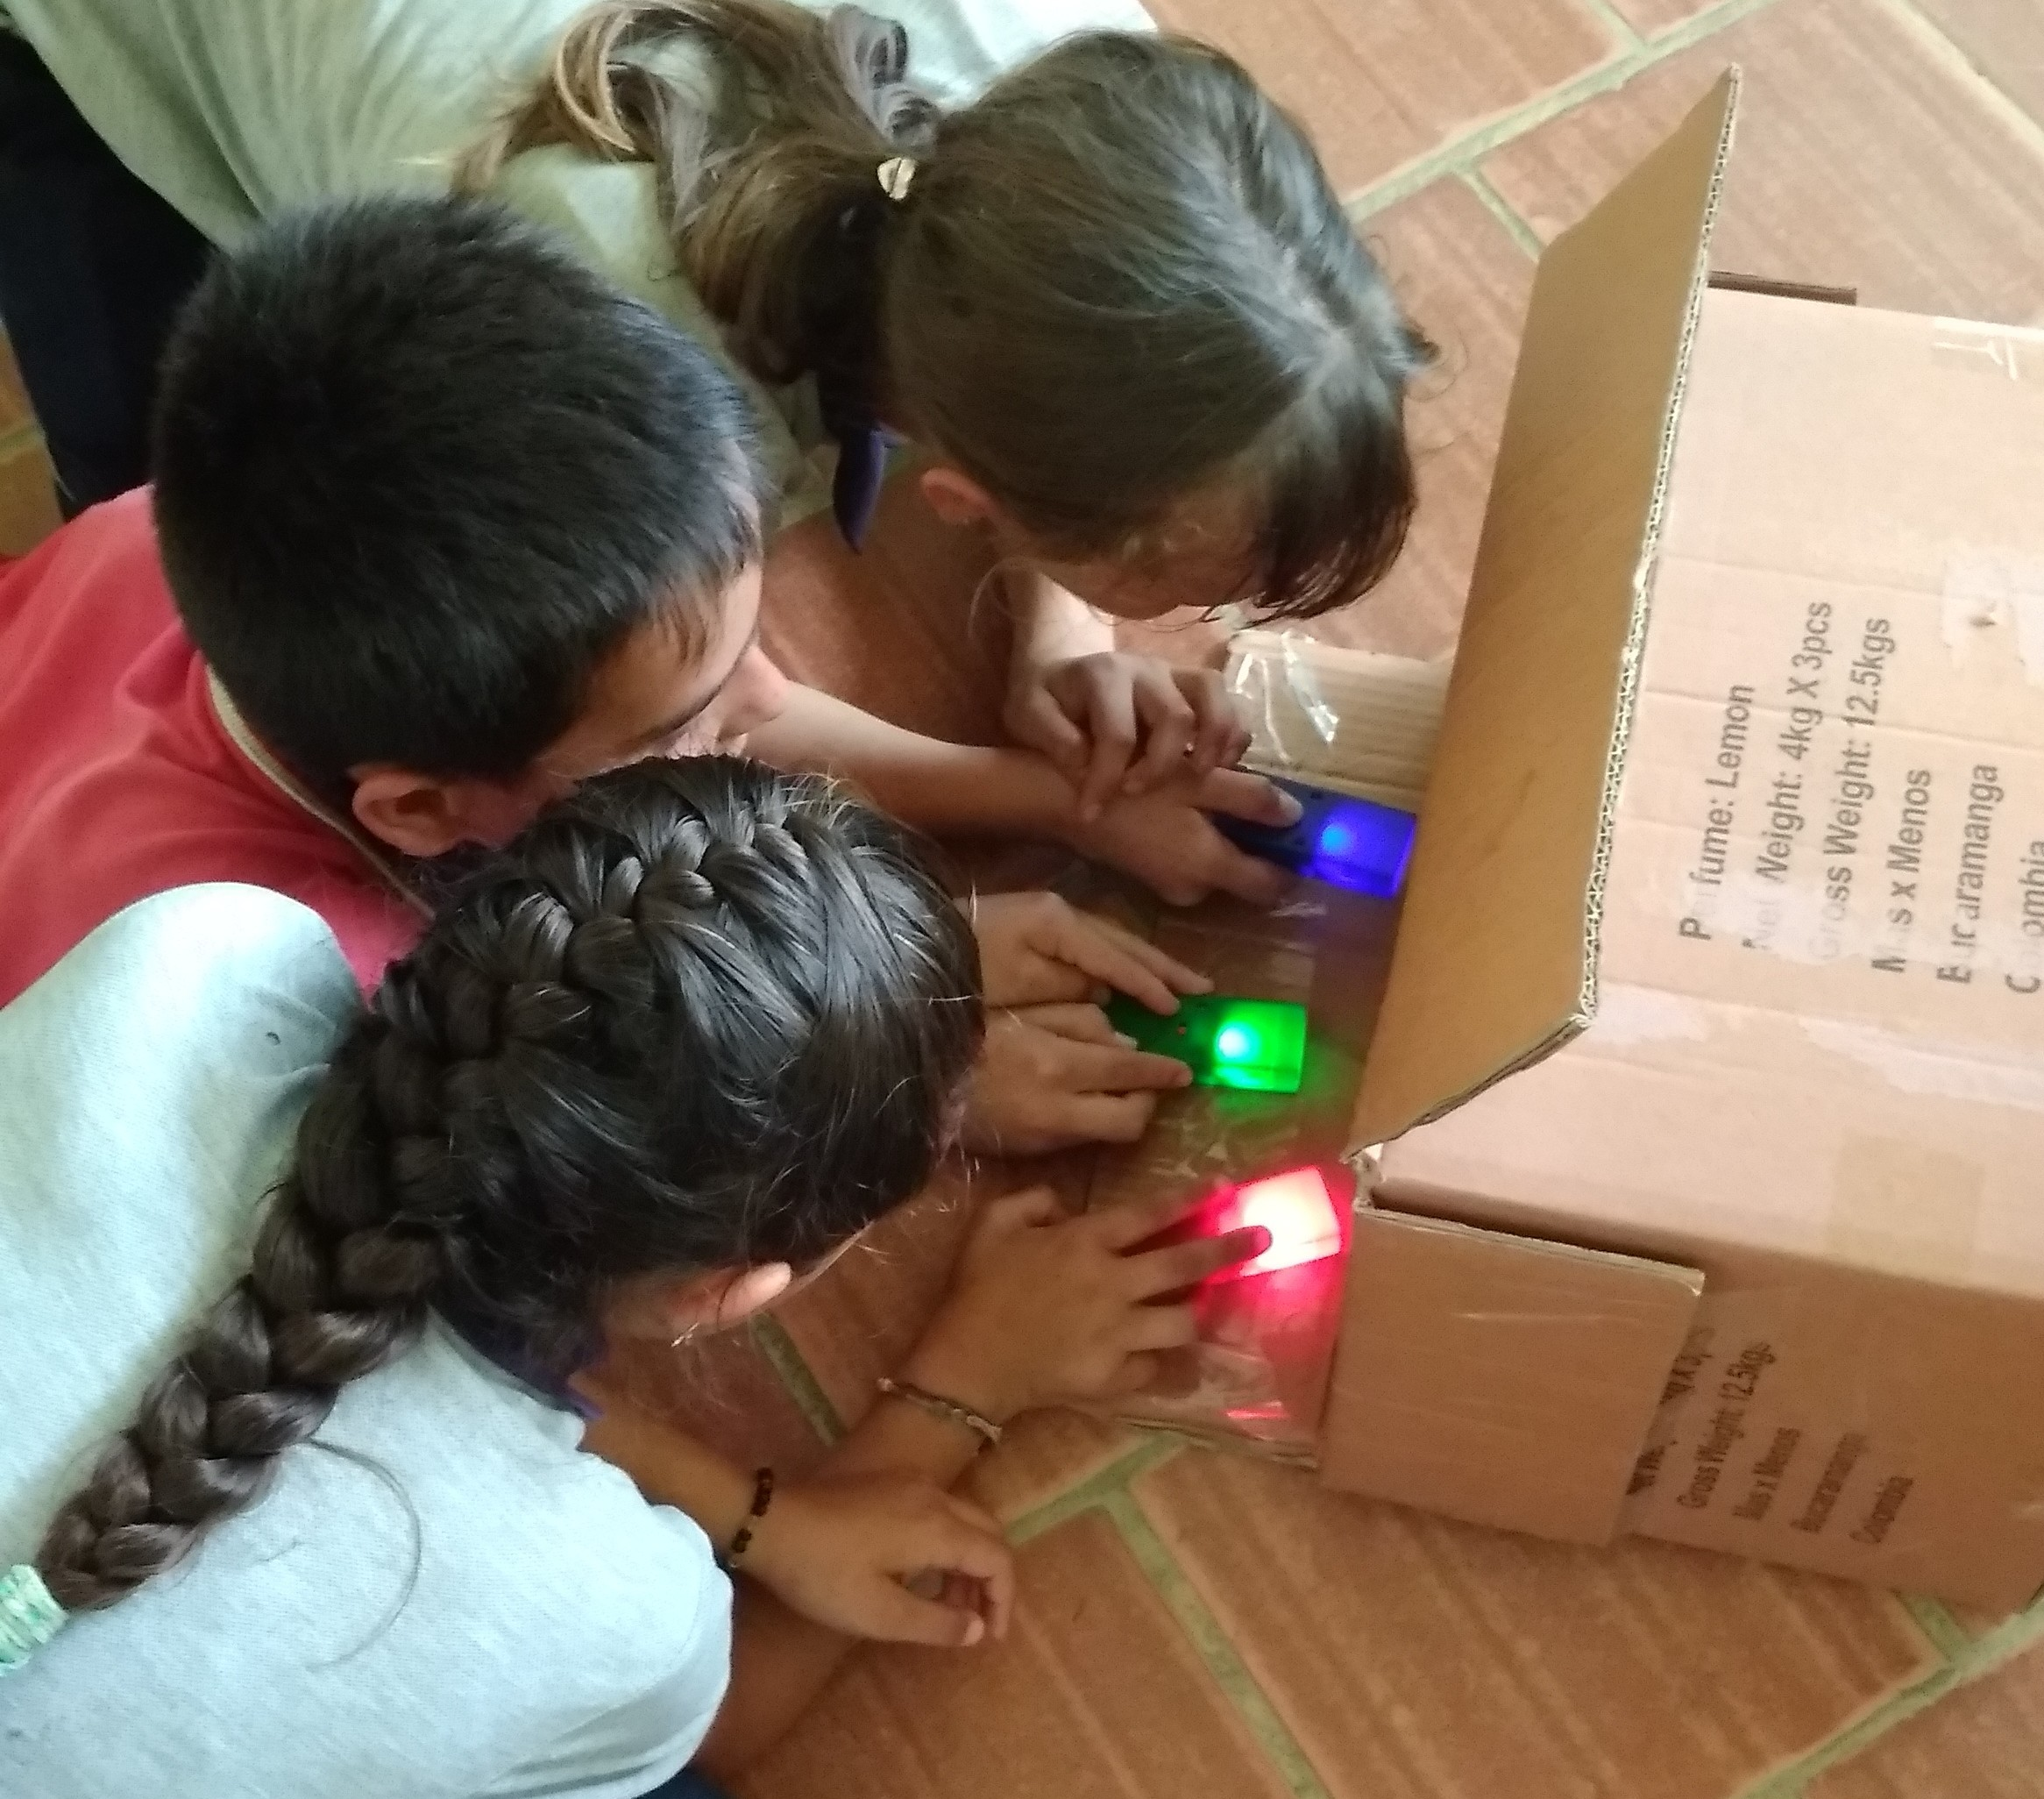
\includegraphics[width = 5.6 cm]{Imagenes/laseresclave.jpg}
    \caption{Formación del color blanco con láser azul, verde y rojo en las Instituciones Educativas El Pórtico (izquierda) y Clavellinas (derecha).}
\end{figure}



\noindent Se habló de las demás componentes del espectro empezando por el infrarrojo, donde se explican sus aplicaciones y se hizo énfasis en la existencia de tipos de luz que normalmente usamos pero son invisibles para los seres humanos. Para ejemplificar esto se tomó una fotografía de un control de TV en funcionamiento con un celular, donde se observó un LED violeta que normalmente no es posible observar.


\begin{figure}[H]
    \centering
    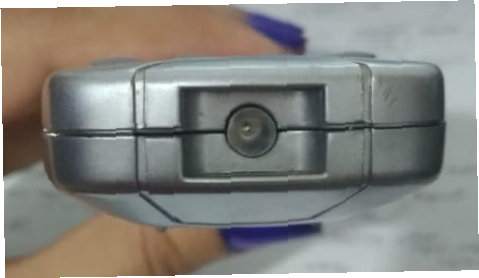
\includegraphics[width = 5.8 cm]{Imagenes/infra2.png}
    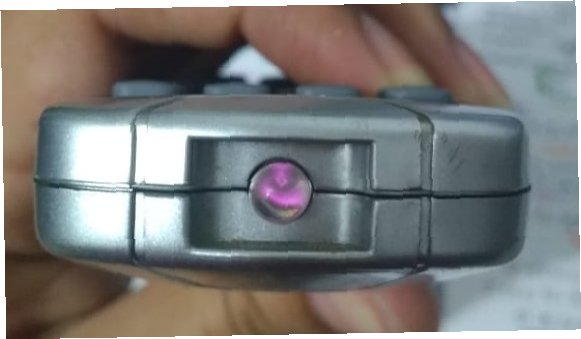
\includegraphics[width = 5.8 cm]{Imagenes/infra.png}
    \caption{Imagen de un control de TV tomada con un celular durante el desarrollo de la actividad en el Colegio San Luis. El sensor de la cámara del celular permite ver la luz infrarroja. 
    }
\end{figure}

\noindent A continuación, se habló del espectro ultravioleta el cual presenta una energía mayor al visible y que por tanto empieza a ser peligroso para la salud humana. En esta sección, se hizo énfasis en la importancia del uso del protector solar para lo cual se mostraron algunos videos grabados con cámara ultravioleta que muestran algunas propiedades de este tipo de radiación y la forma en que fue descubierta. \\


\begin{figure}[H]
    \centering
    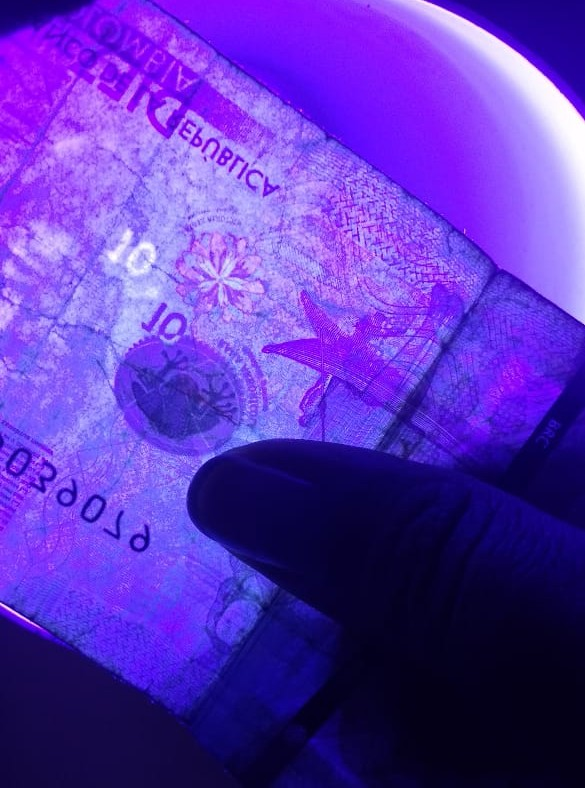
\includegraphics[height=5.8cm]{Imagenes/uv1.jpeg}
    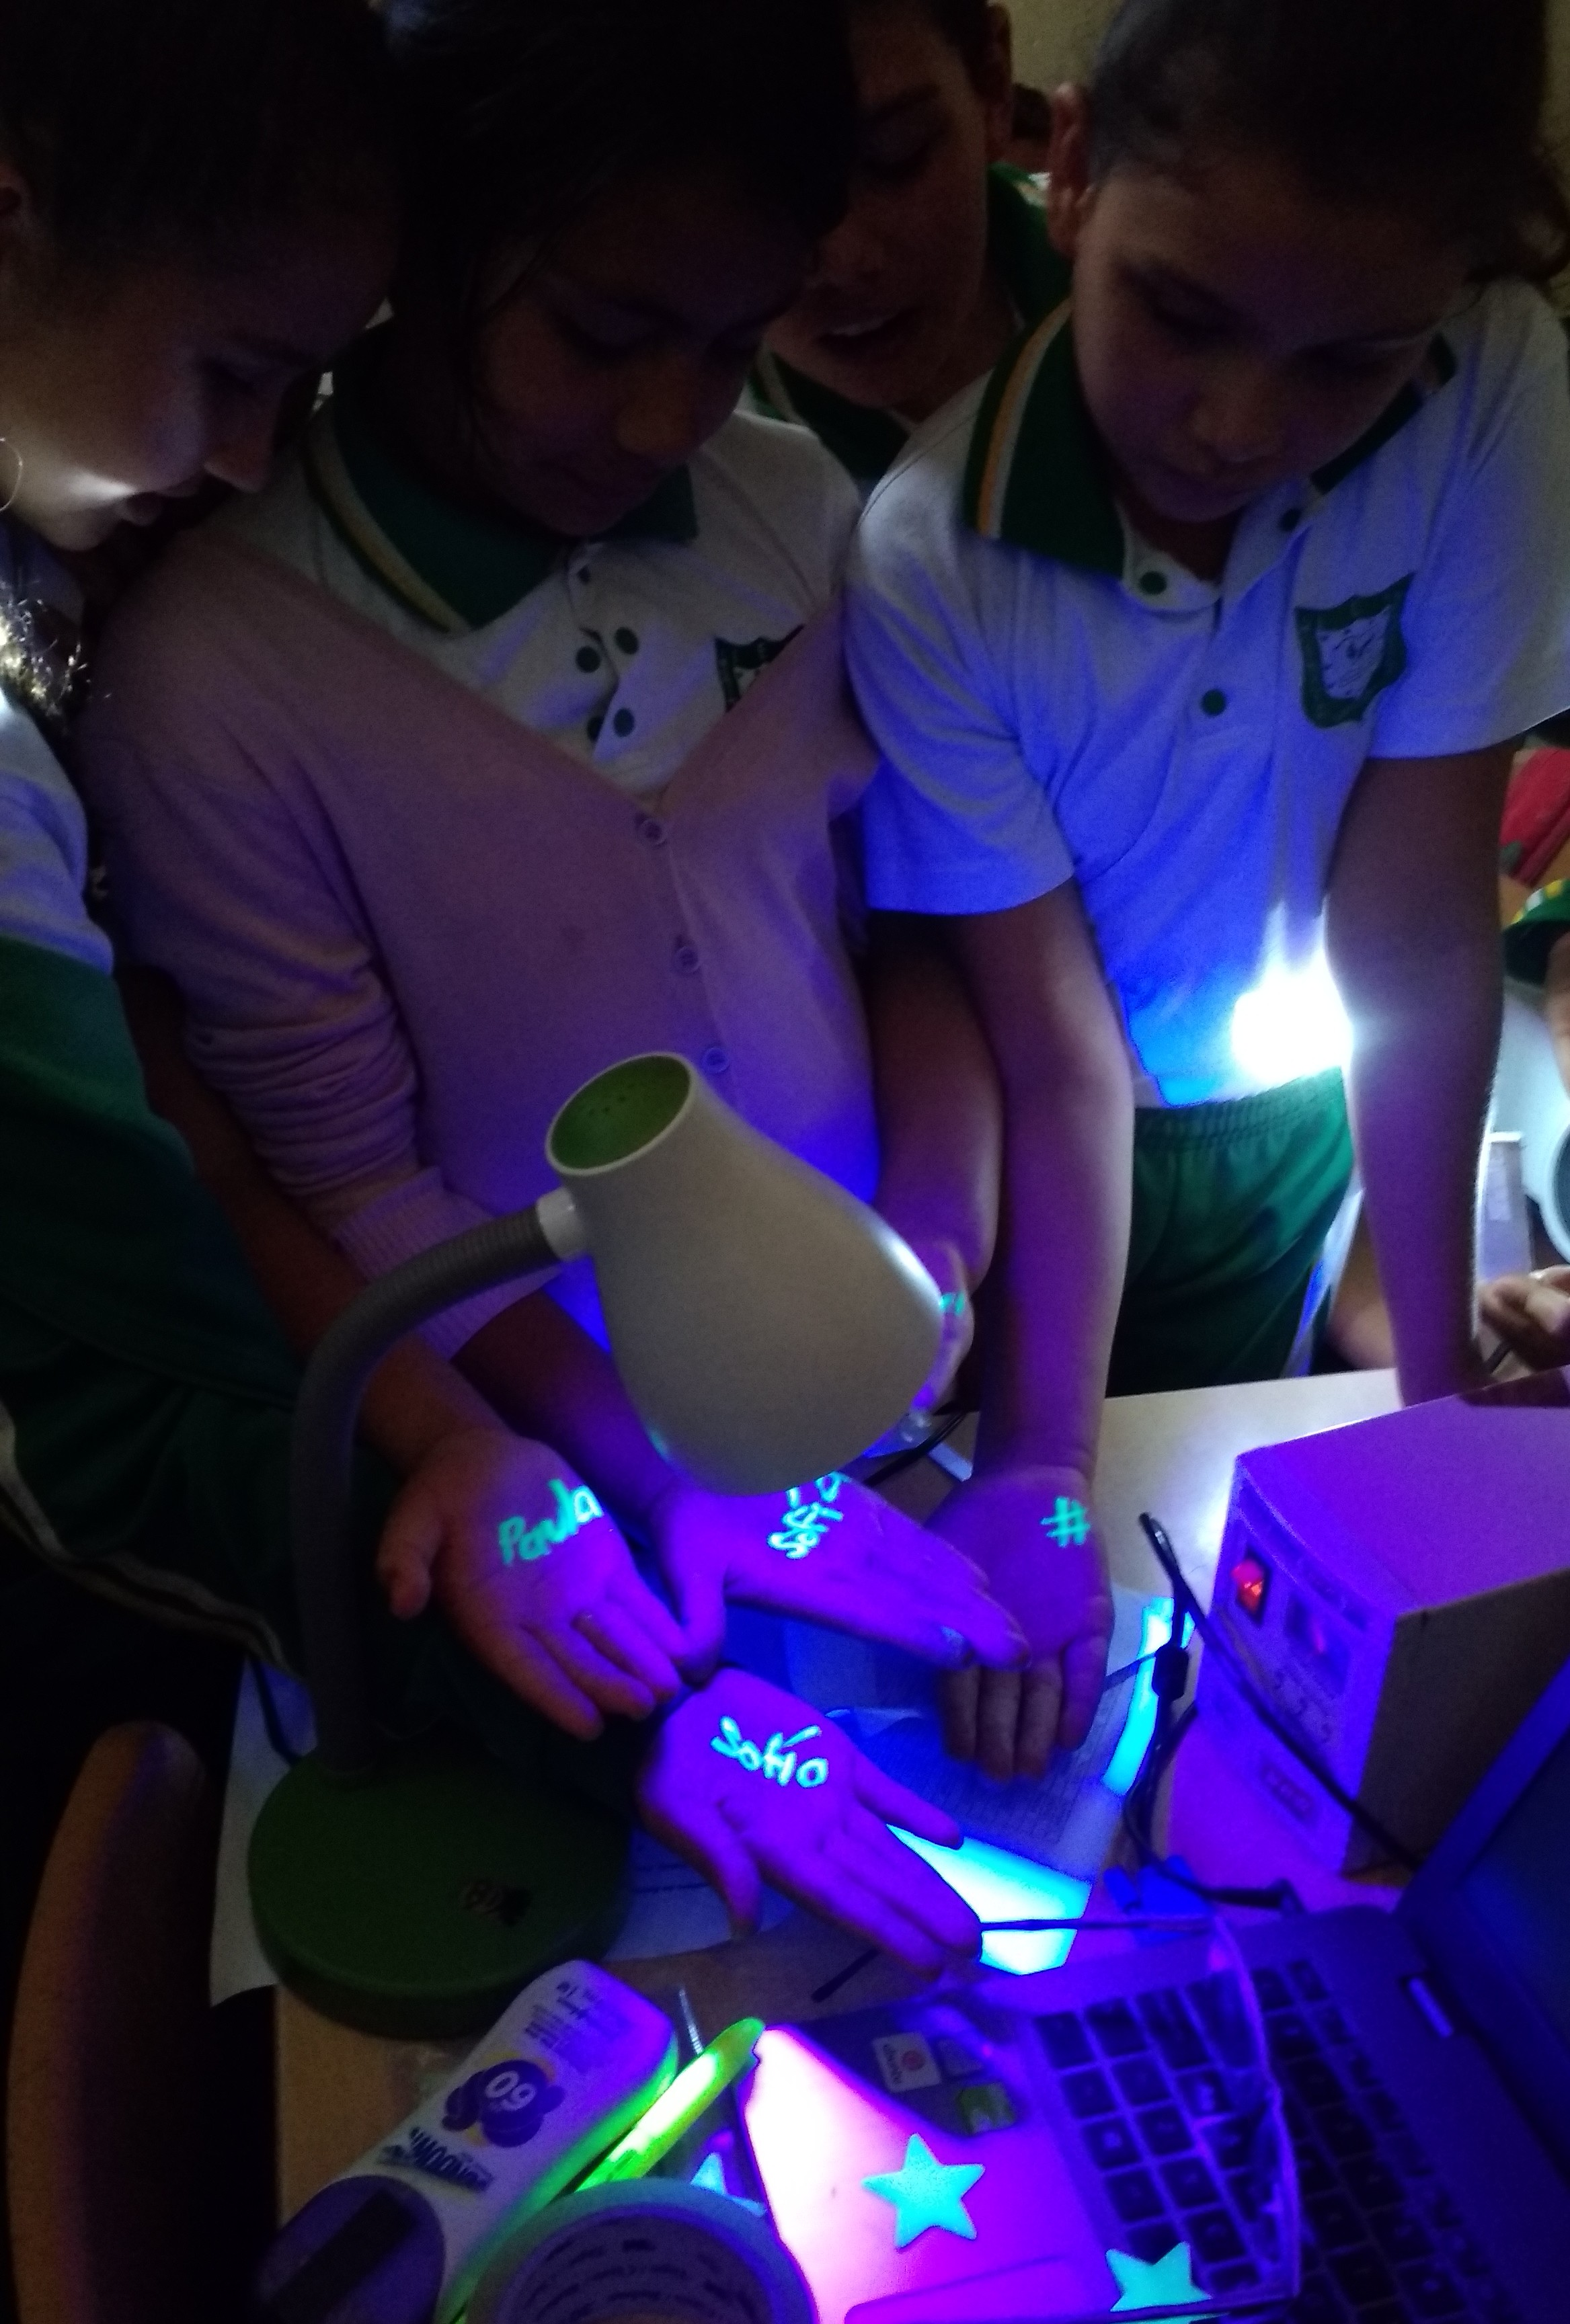
\includegraphics[height=5.8cm]{Imagenes/ultraportico.jpg}
    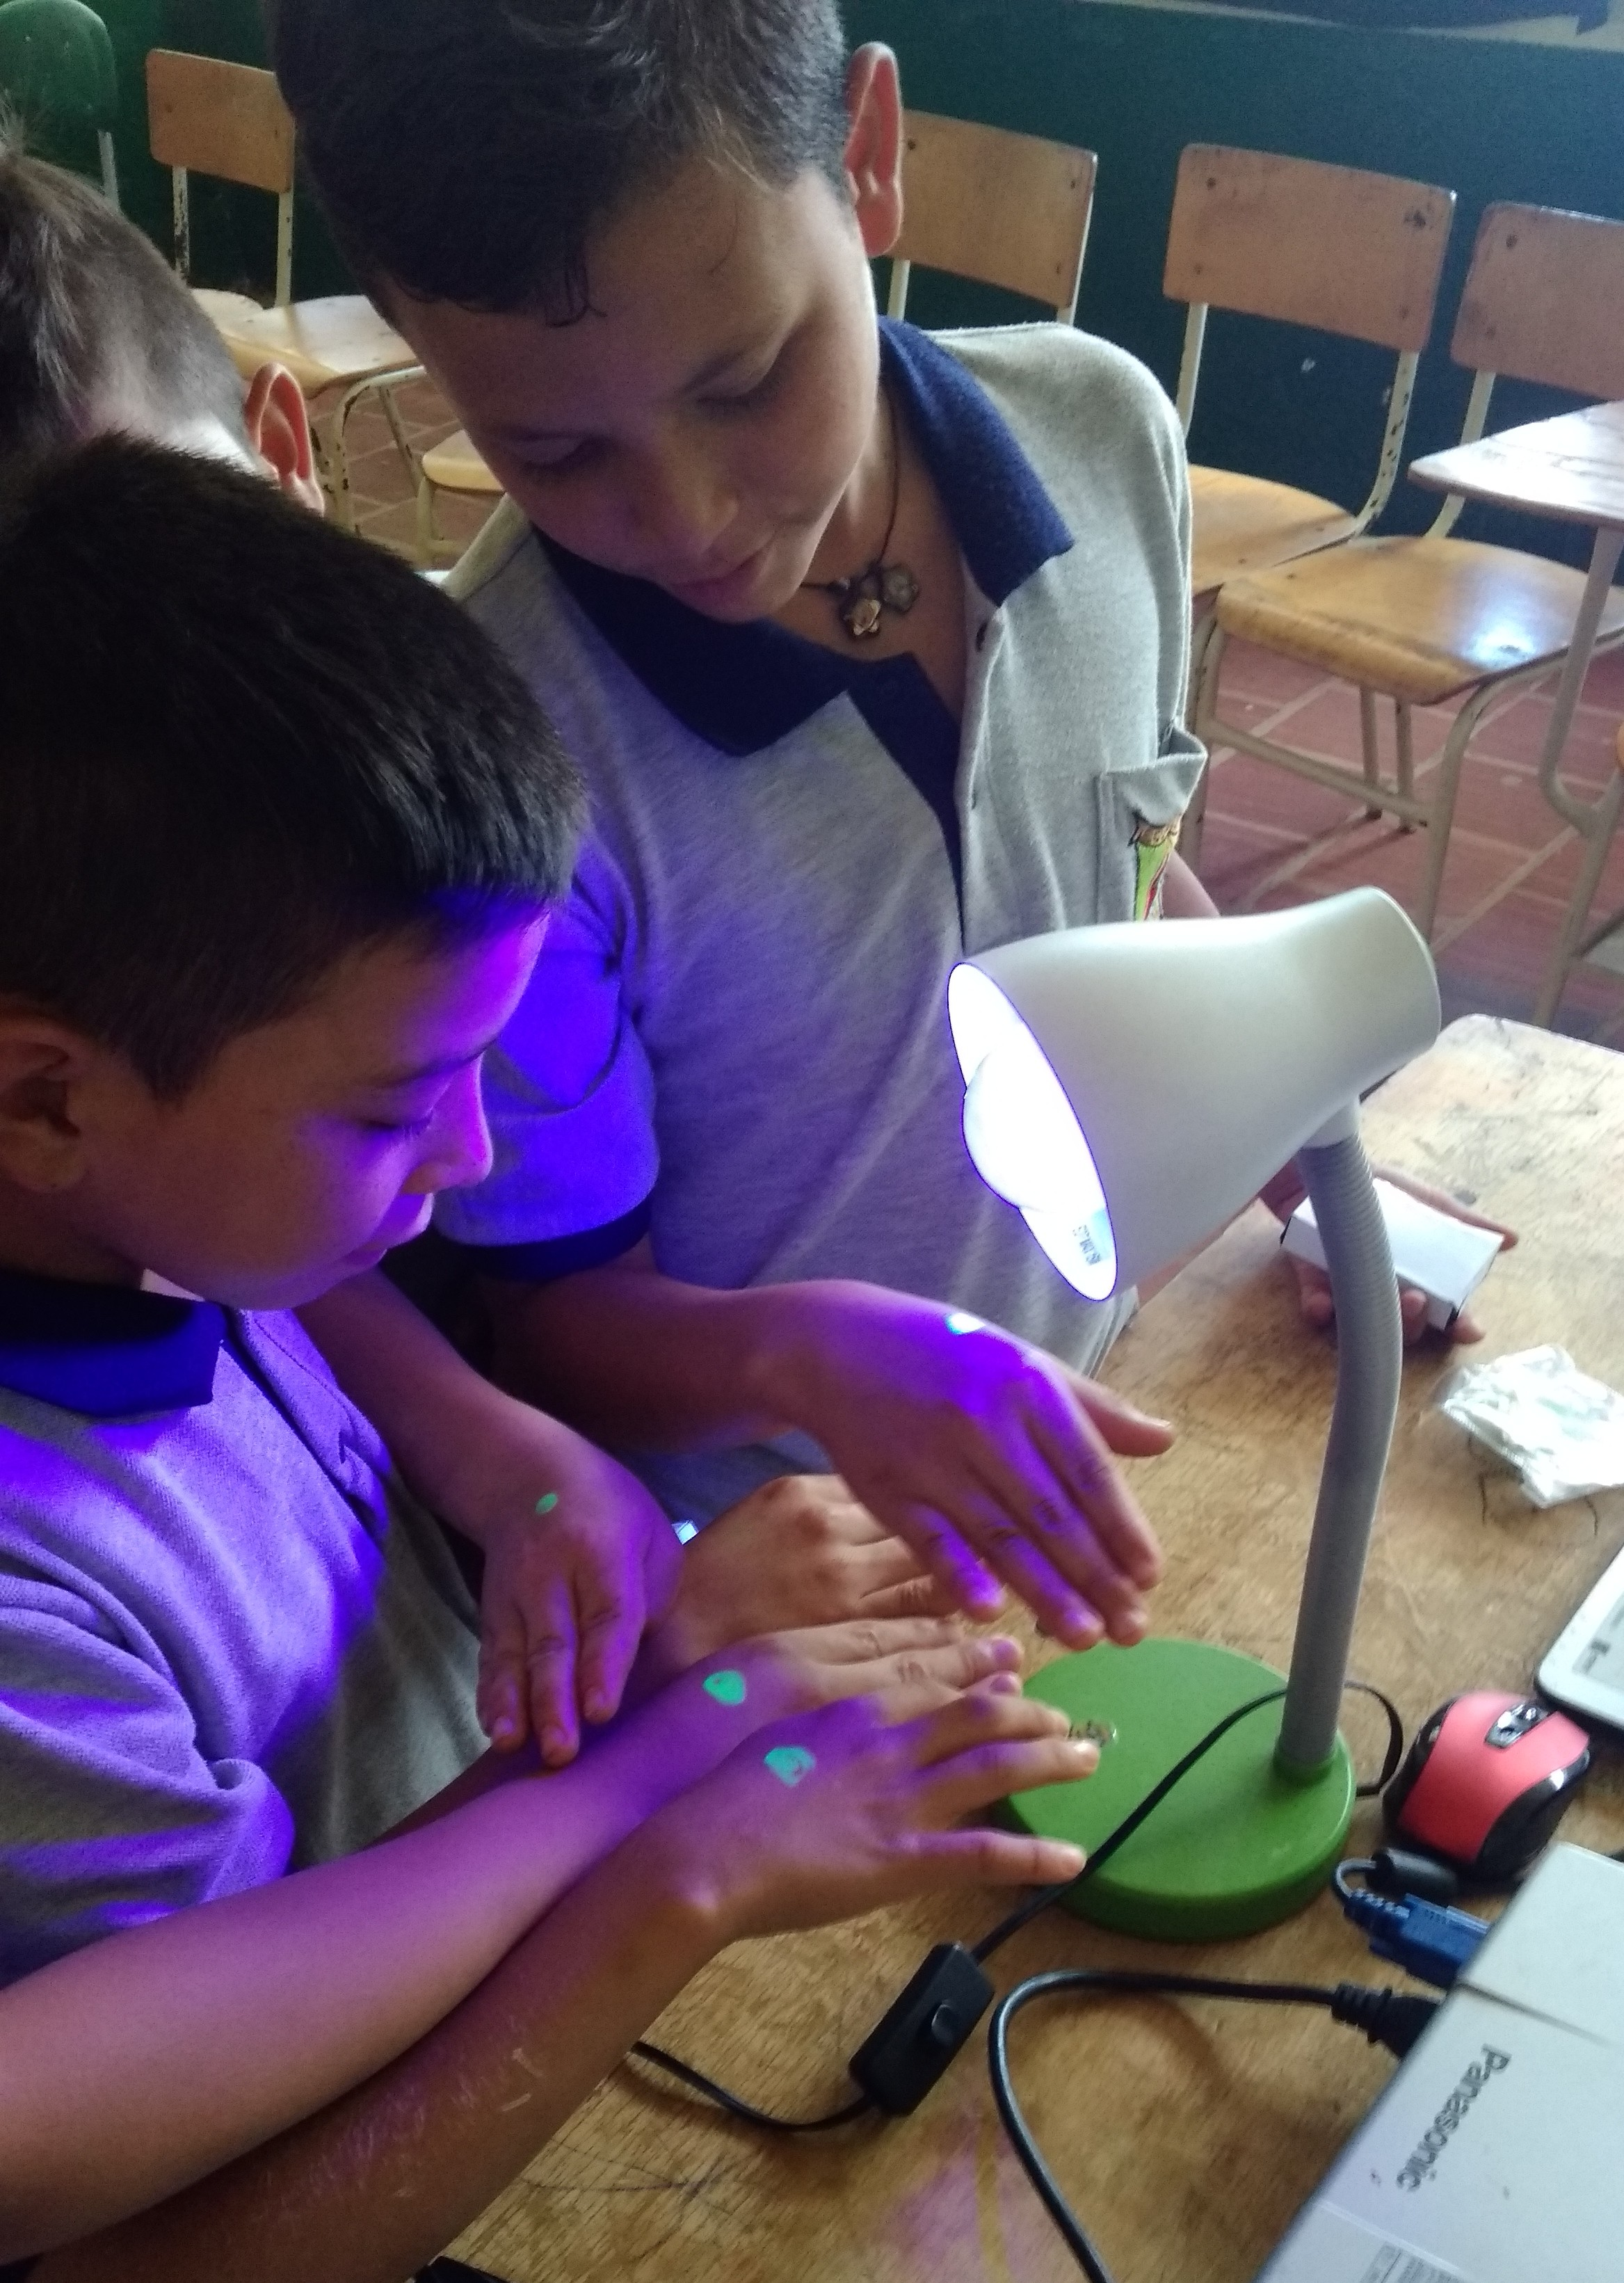
\includegraphics[height=5.8cm]{Imagenes/ultraclave.jpg}
    
    \caption{Diferentes aplicaciones de la luz ultravioleta: identificar veracidad de los billetes, observar con mayor intensidad objetos fluorescentes y evidenciar la protección ante los rayos UV brindada por las gafas y el bloqueador. Imágenes de las actividades desarrolladas en el Colegio San Luis (izquierda), en la Institución Educativa El Pórtico (centro) y en la Institución Educativa Clavellinas (derecha). }
\end{figure}

\noindent Para profundizar en estos conceptos se hizo uso de una lámpara ultravioleta con la que se probaron la veracidad de algunos billetes, se probaron diferentes materiales sensibles al ultravioleta como los resaltadores comúnes y unas estrellas fluorescentes y además se observó la protección brindada por el bloqueador solar y unas gafas de vidrio común. Finalmente, se abordaron las últimas dos componentes del espectro electromagnético que consiste en los rayos X y los rayos gamma. Debido a la alta energía de estos tipos de radiación no fue posible realizar algún experimento que permitiera evidenciarlos. Sin embargo se mostraron algunas aplicaciones y se explicaron las posibles fuentes de estos tipos de radiaciones en eventos extragalácticos como fusiones de galaxias, super novas y eventos energéticos similares.\\



\noindent \textbf{Fenómenos de la luz (1 hora y 40 minutos)}\\


\noindent En la última parte se estudian los fenómenos y propiedades de la luz. Se empieza explicando el fenómeno de dispersión y el estudio realizado por Newton; además, se da respuesta a preguntas tales como: ¿Por qué el cielo es azul? ¿Por qué se observa el arcoíris? y ¿Cuándo ocurre el fenómeno de dispersión? La dinámica para comprender la dispersión se realizó con el uso de un prisma, en esta parte los estudiantes pudieron manipular el prisma y de esta forma lograron observar la separación de la luz blanca en sus componentes espectrales. También con la dispersión de la luz en una barra de silicona se explicó la dispersión de Rayleigh causante del cielo rojizo al atardecer y el amanecer.\\

\begin{figure}[H]
    \centering
    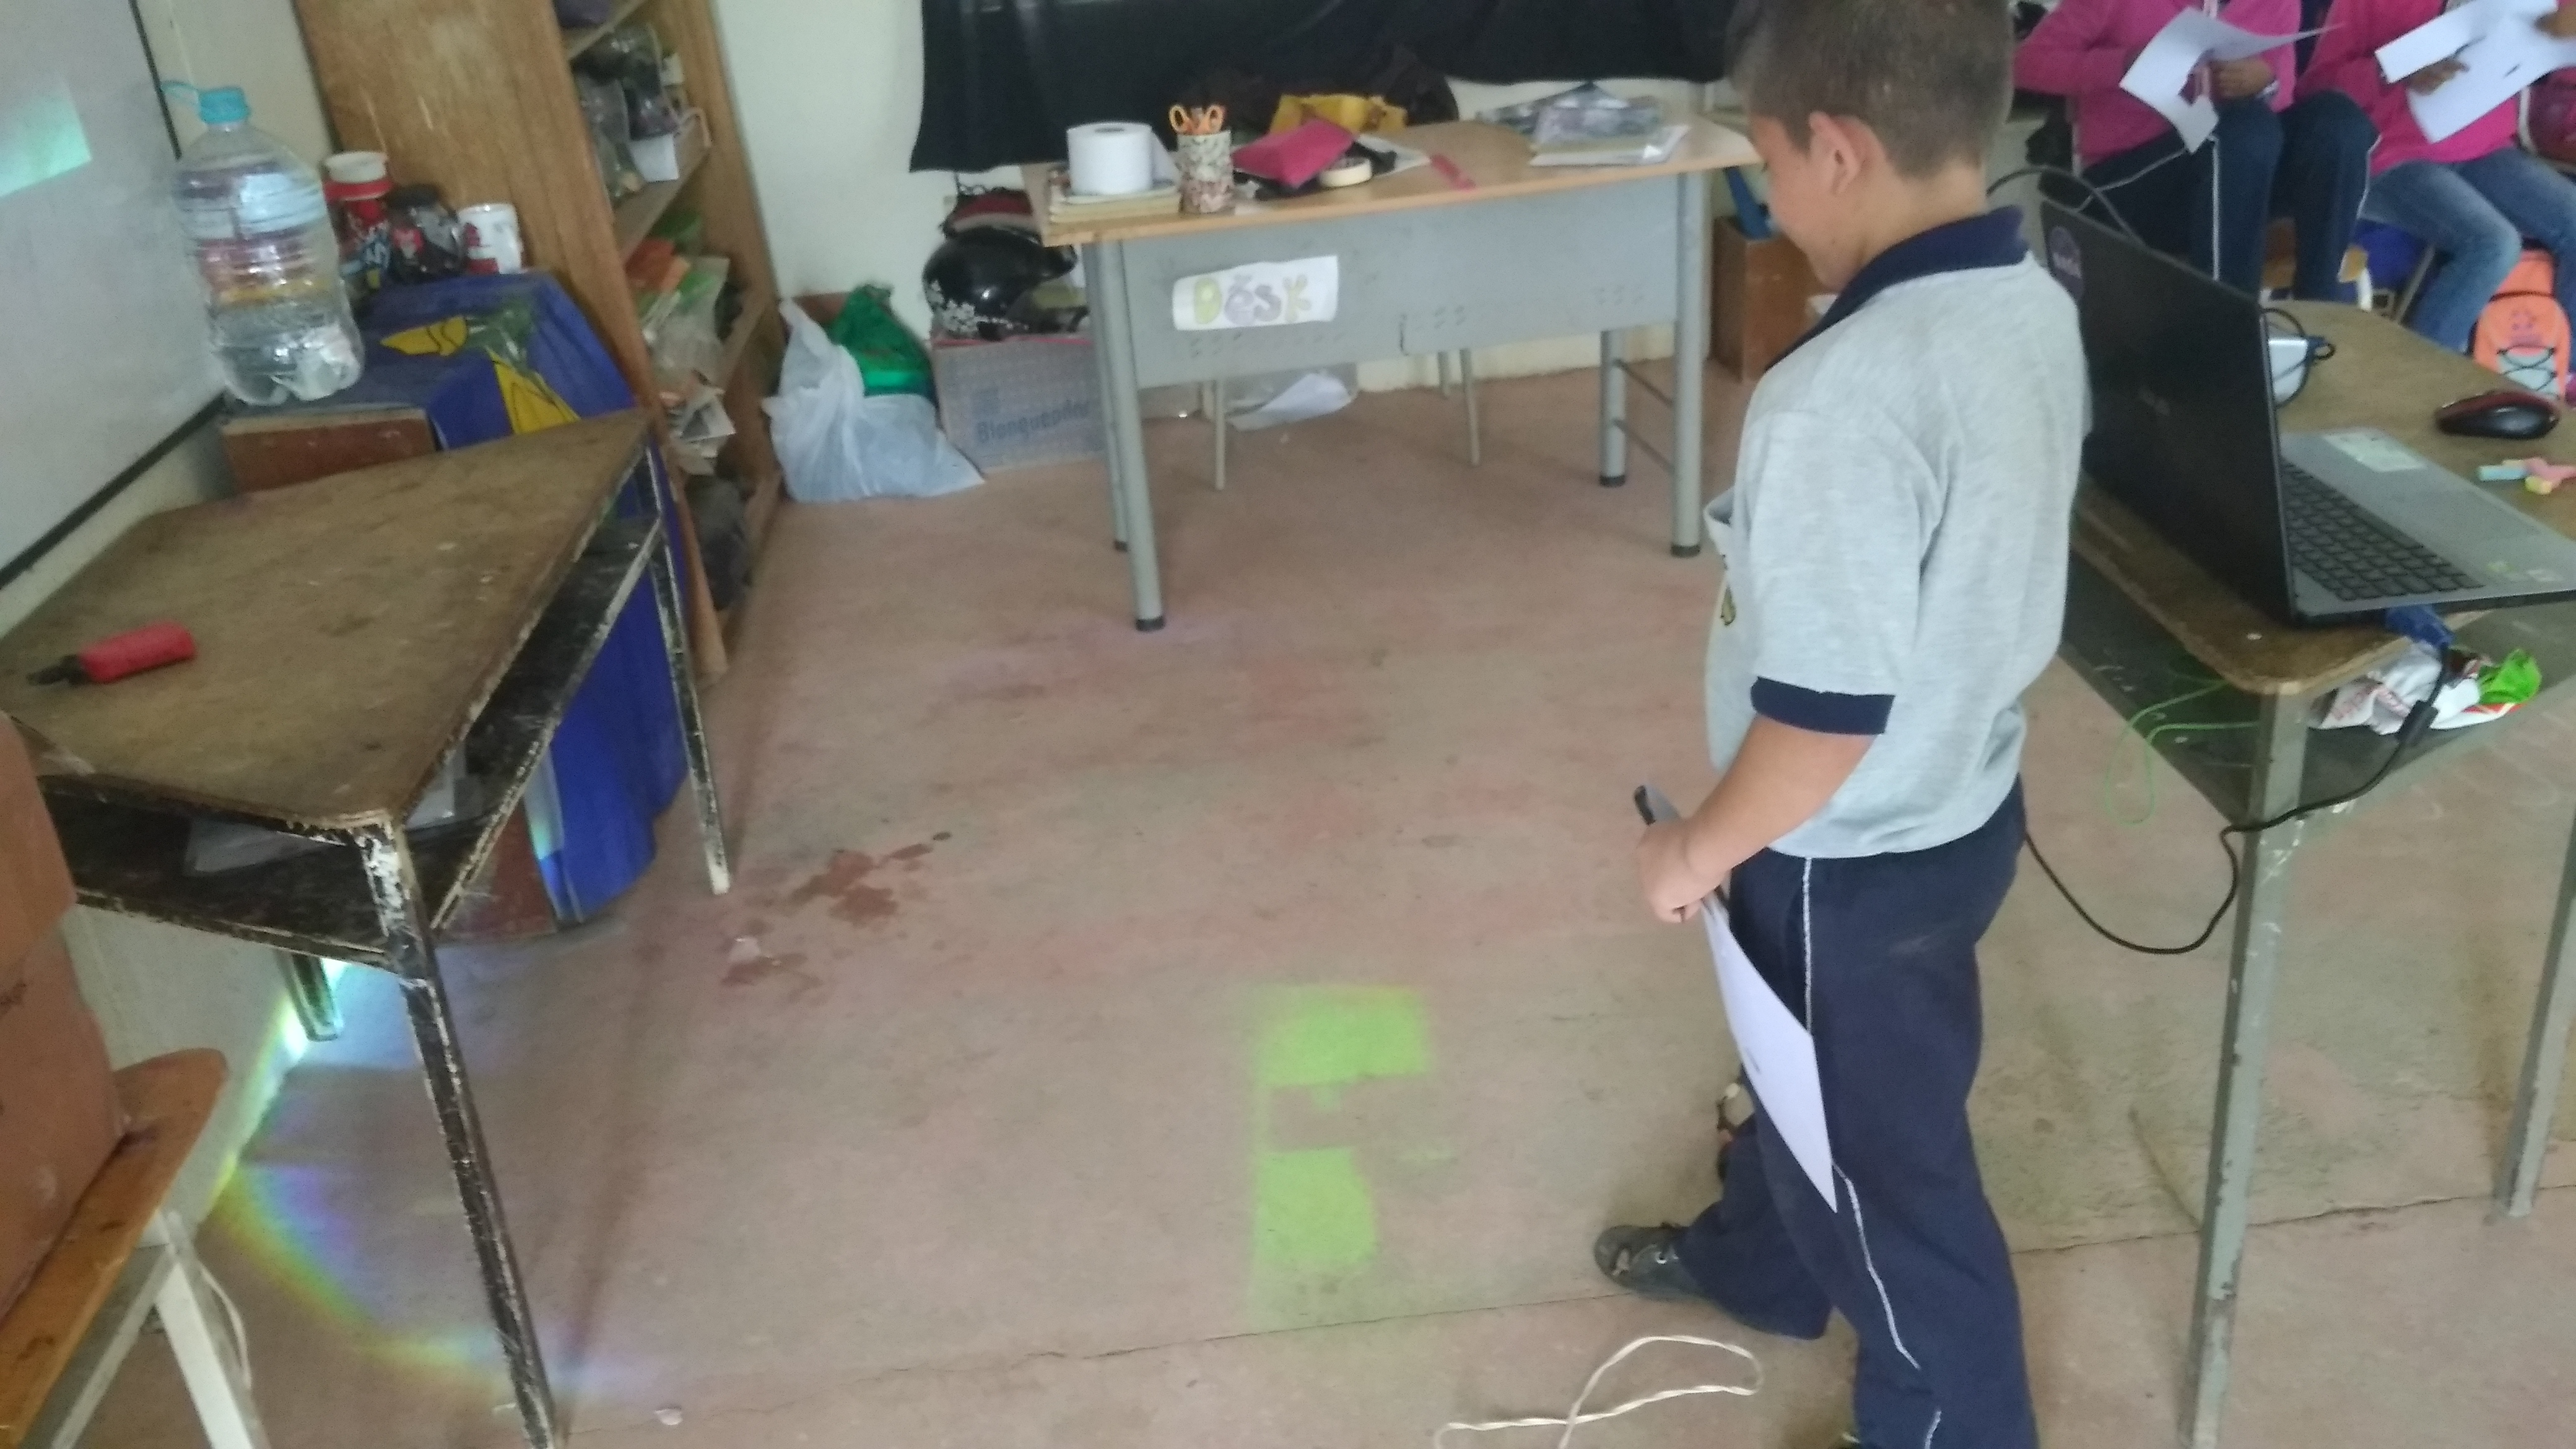
\includegraphics[height=5cm]{Imagenes/prismaclave.jpg}
    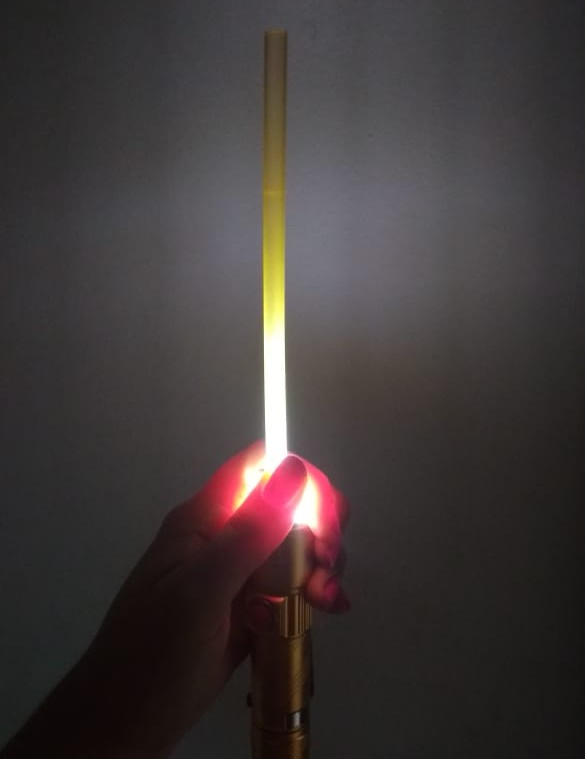
\includegraphics[height=5cm]{Imagenes/rayleigh1.jpeg}
    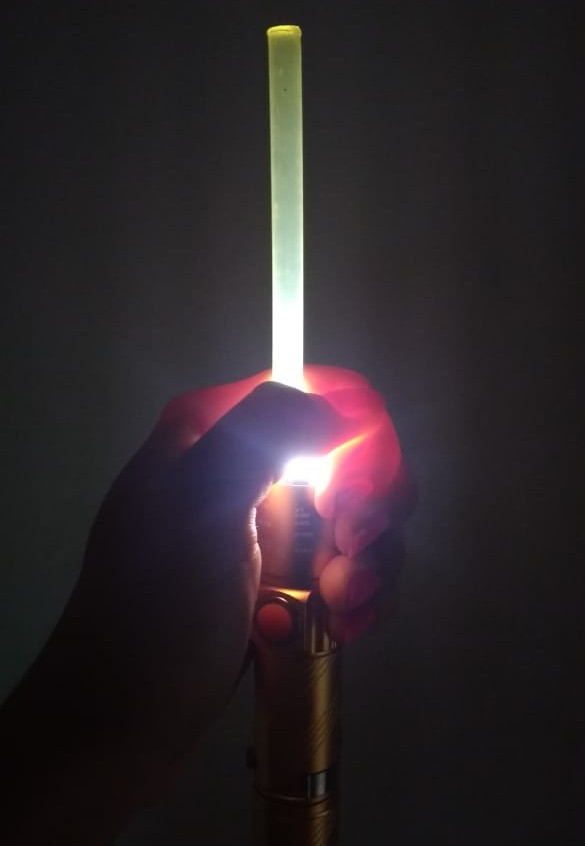
\includegraphics[height=5cm]{Imagenes/rayleigh2.jpeg}
    \caption{Descomposición de la luz usando un prisma y vídeo beam en la Institución Educativa Clavellinas (izquierda) y actividad de dispersión de Rayleigh realizada en el Colegio San Luis (centro y derecha).}
\end{figure}

\noindent Posteriormente, se realizó el estudio de la refracción y reflexión de la luz debido al cambio de medio en el que esta se propaga. Las dinámicas que se realizaron fueron: la observación de la trayectoria de un láser cuando se somete al cambio de varios medios de propagación y la observación de la imagen proveniente de un lápiz sumergido en diferentes tipos de sustancias. Con el desarrollo de esta actividad los estudiantes comprendieron los efectos del índice de refracción y la desviación de la luz, igualmente comprendieron el fenómeno de reflexión que se presenta ante cambios de medios.\\

\begin{figure}[H]
    \centering
    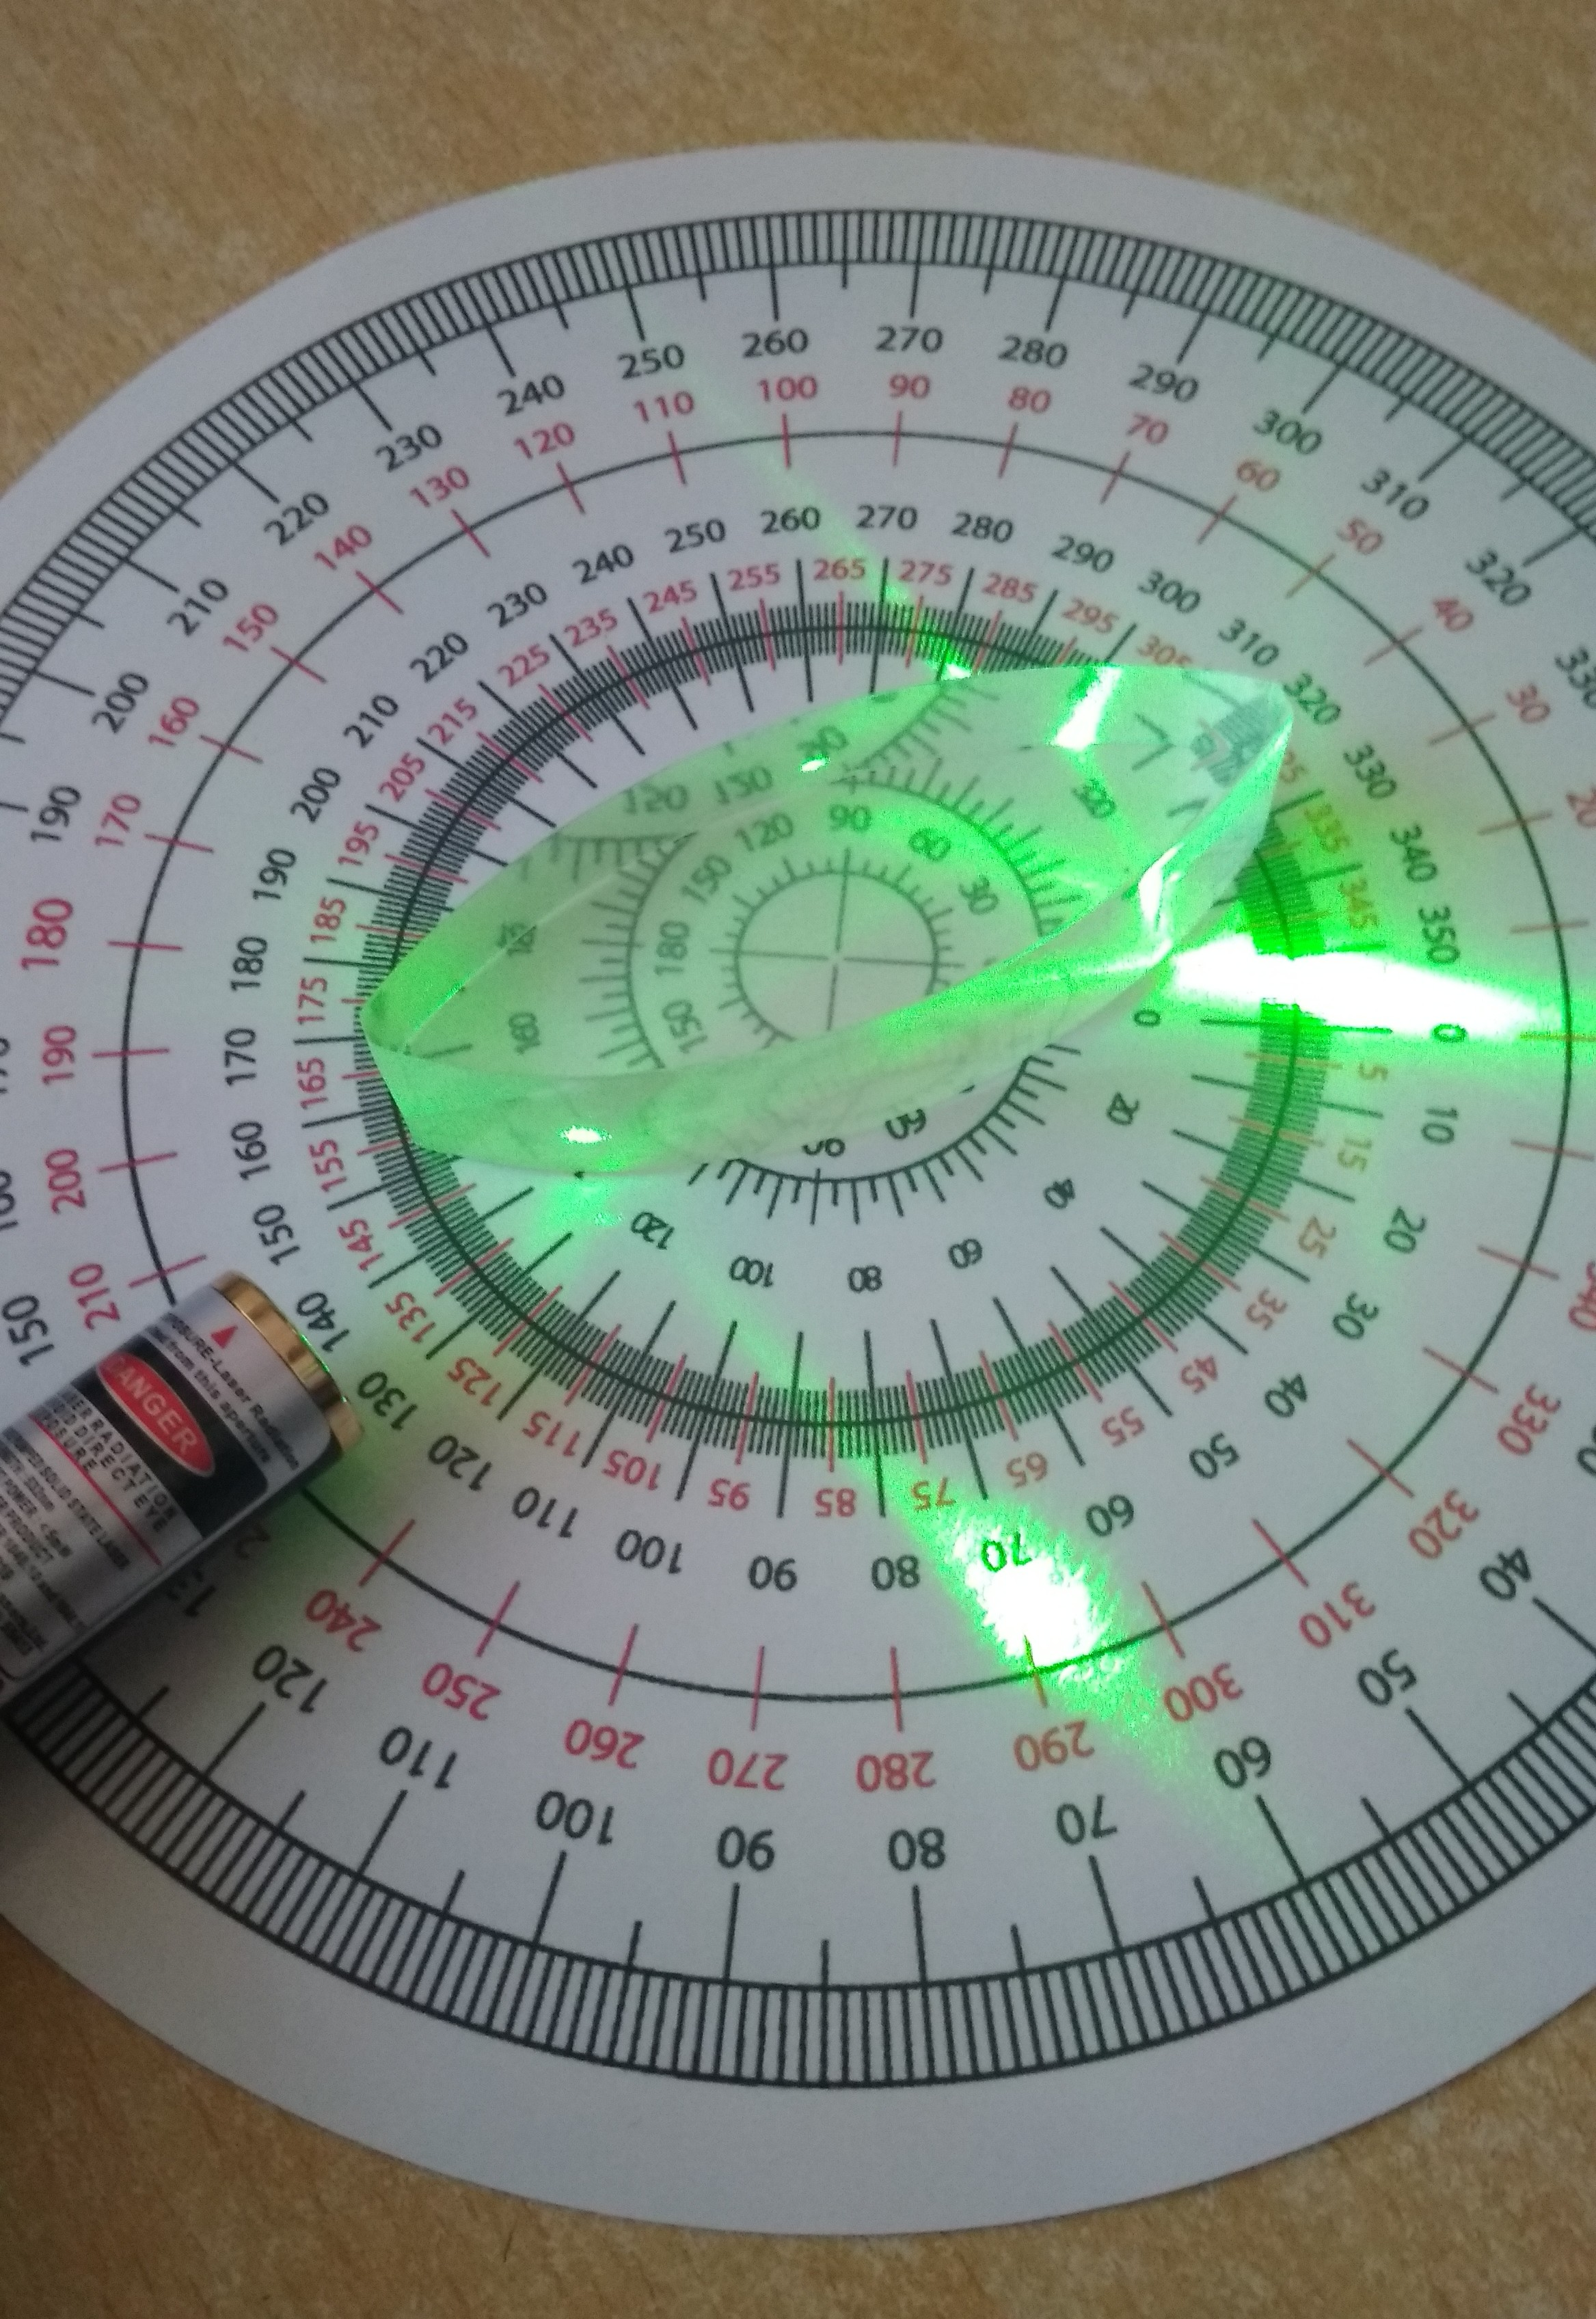
\includegraphics[height=5cm]{Imagenes/laserlente.jpg}
    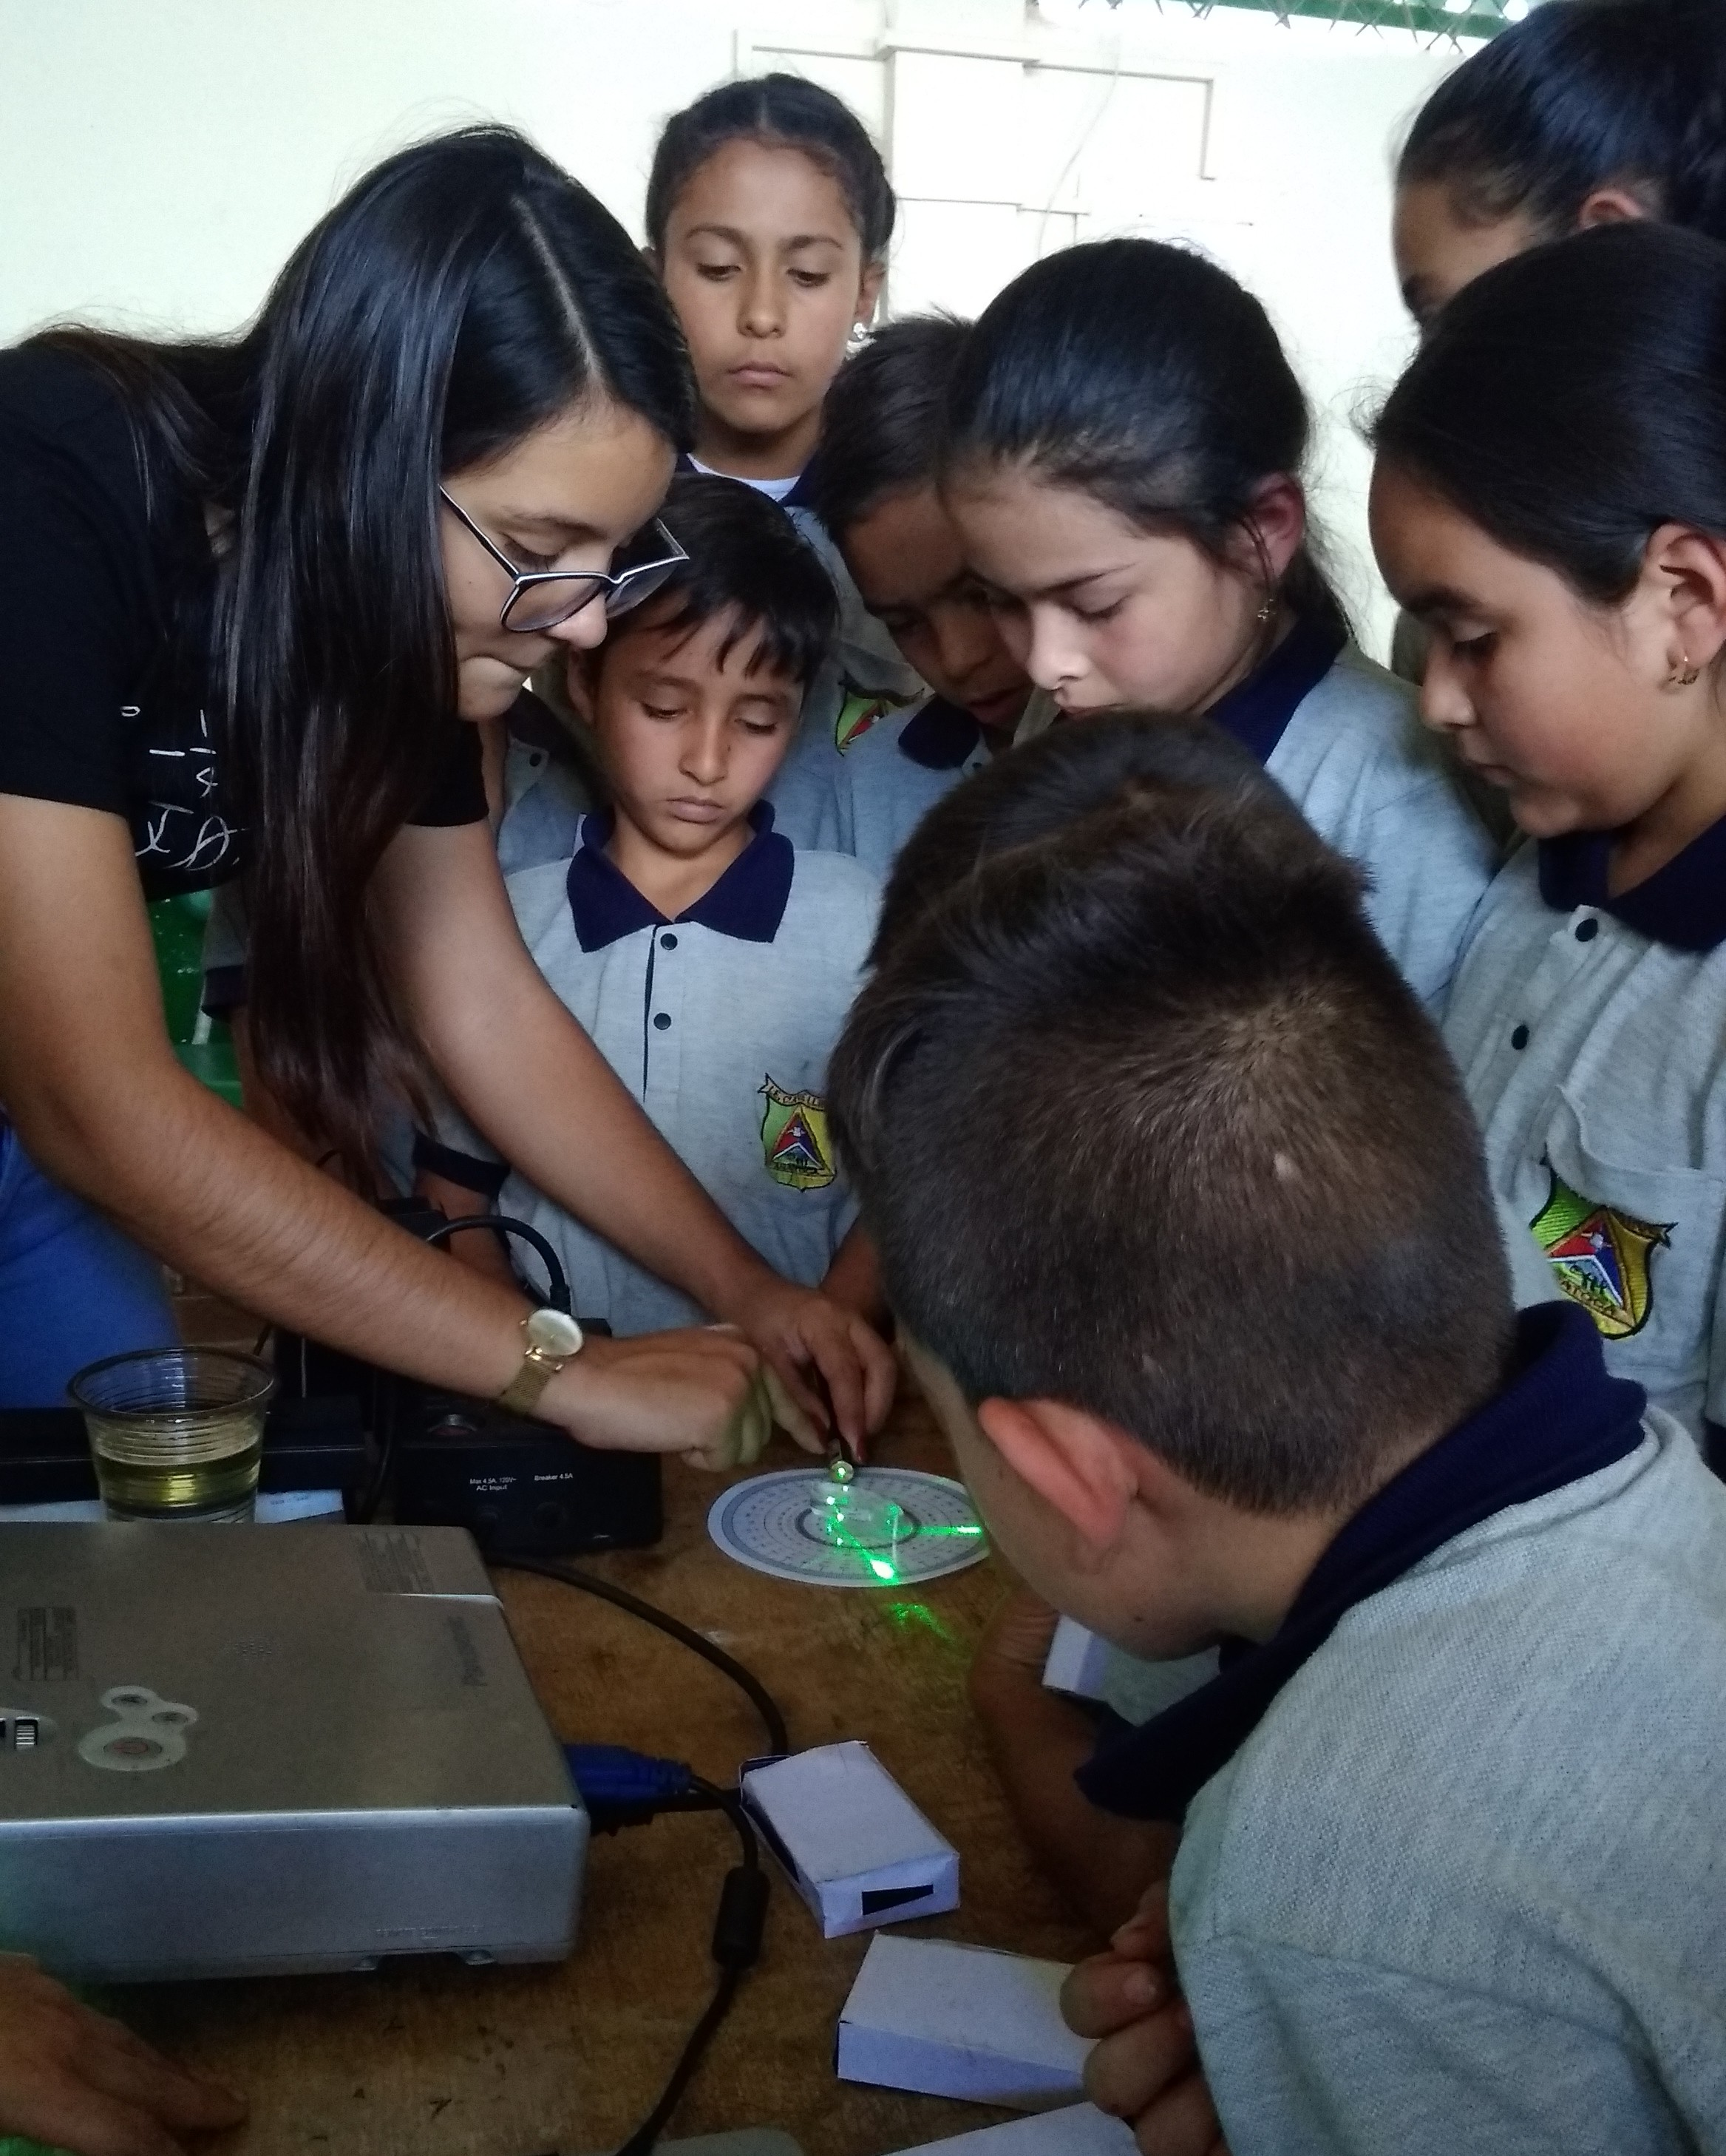
\includegraphics[height=5cm]{Imagenes/laserclave.jpg}
    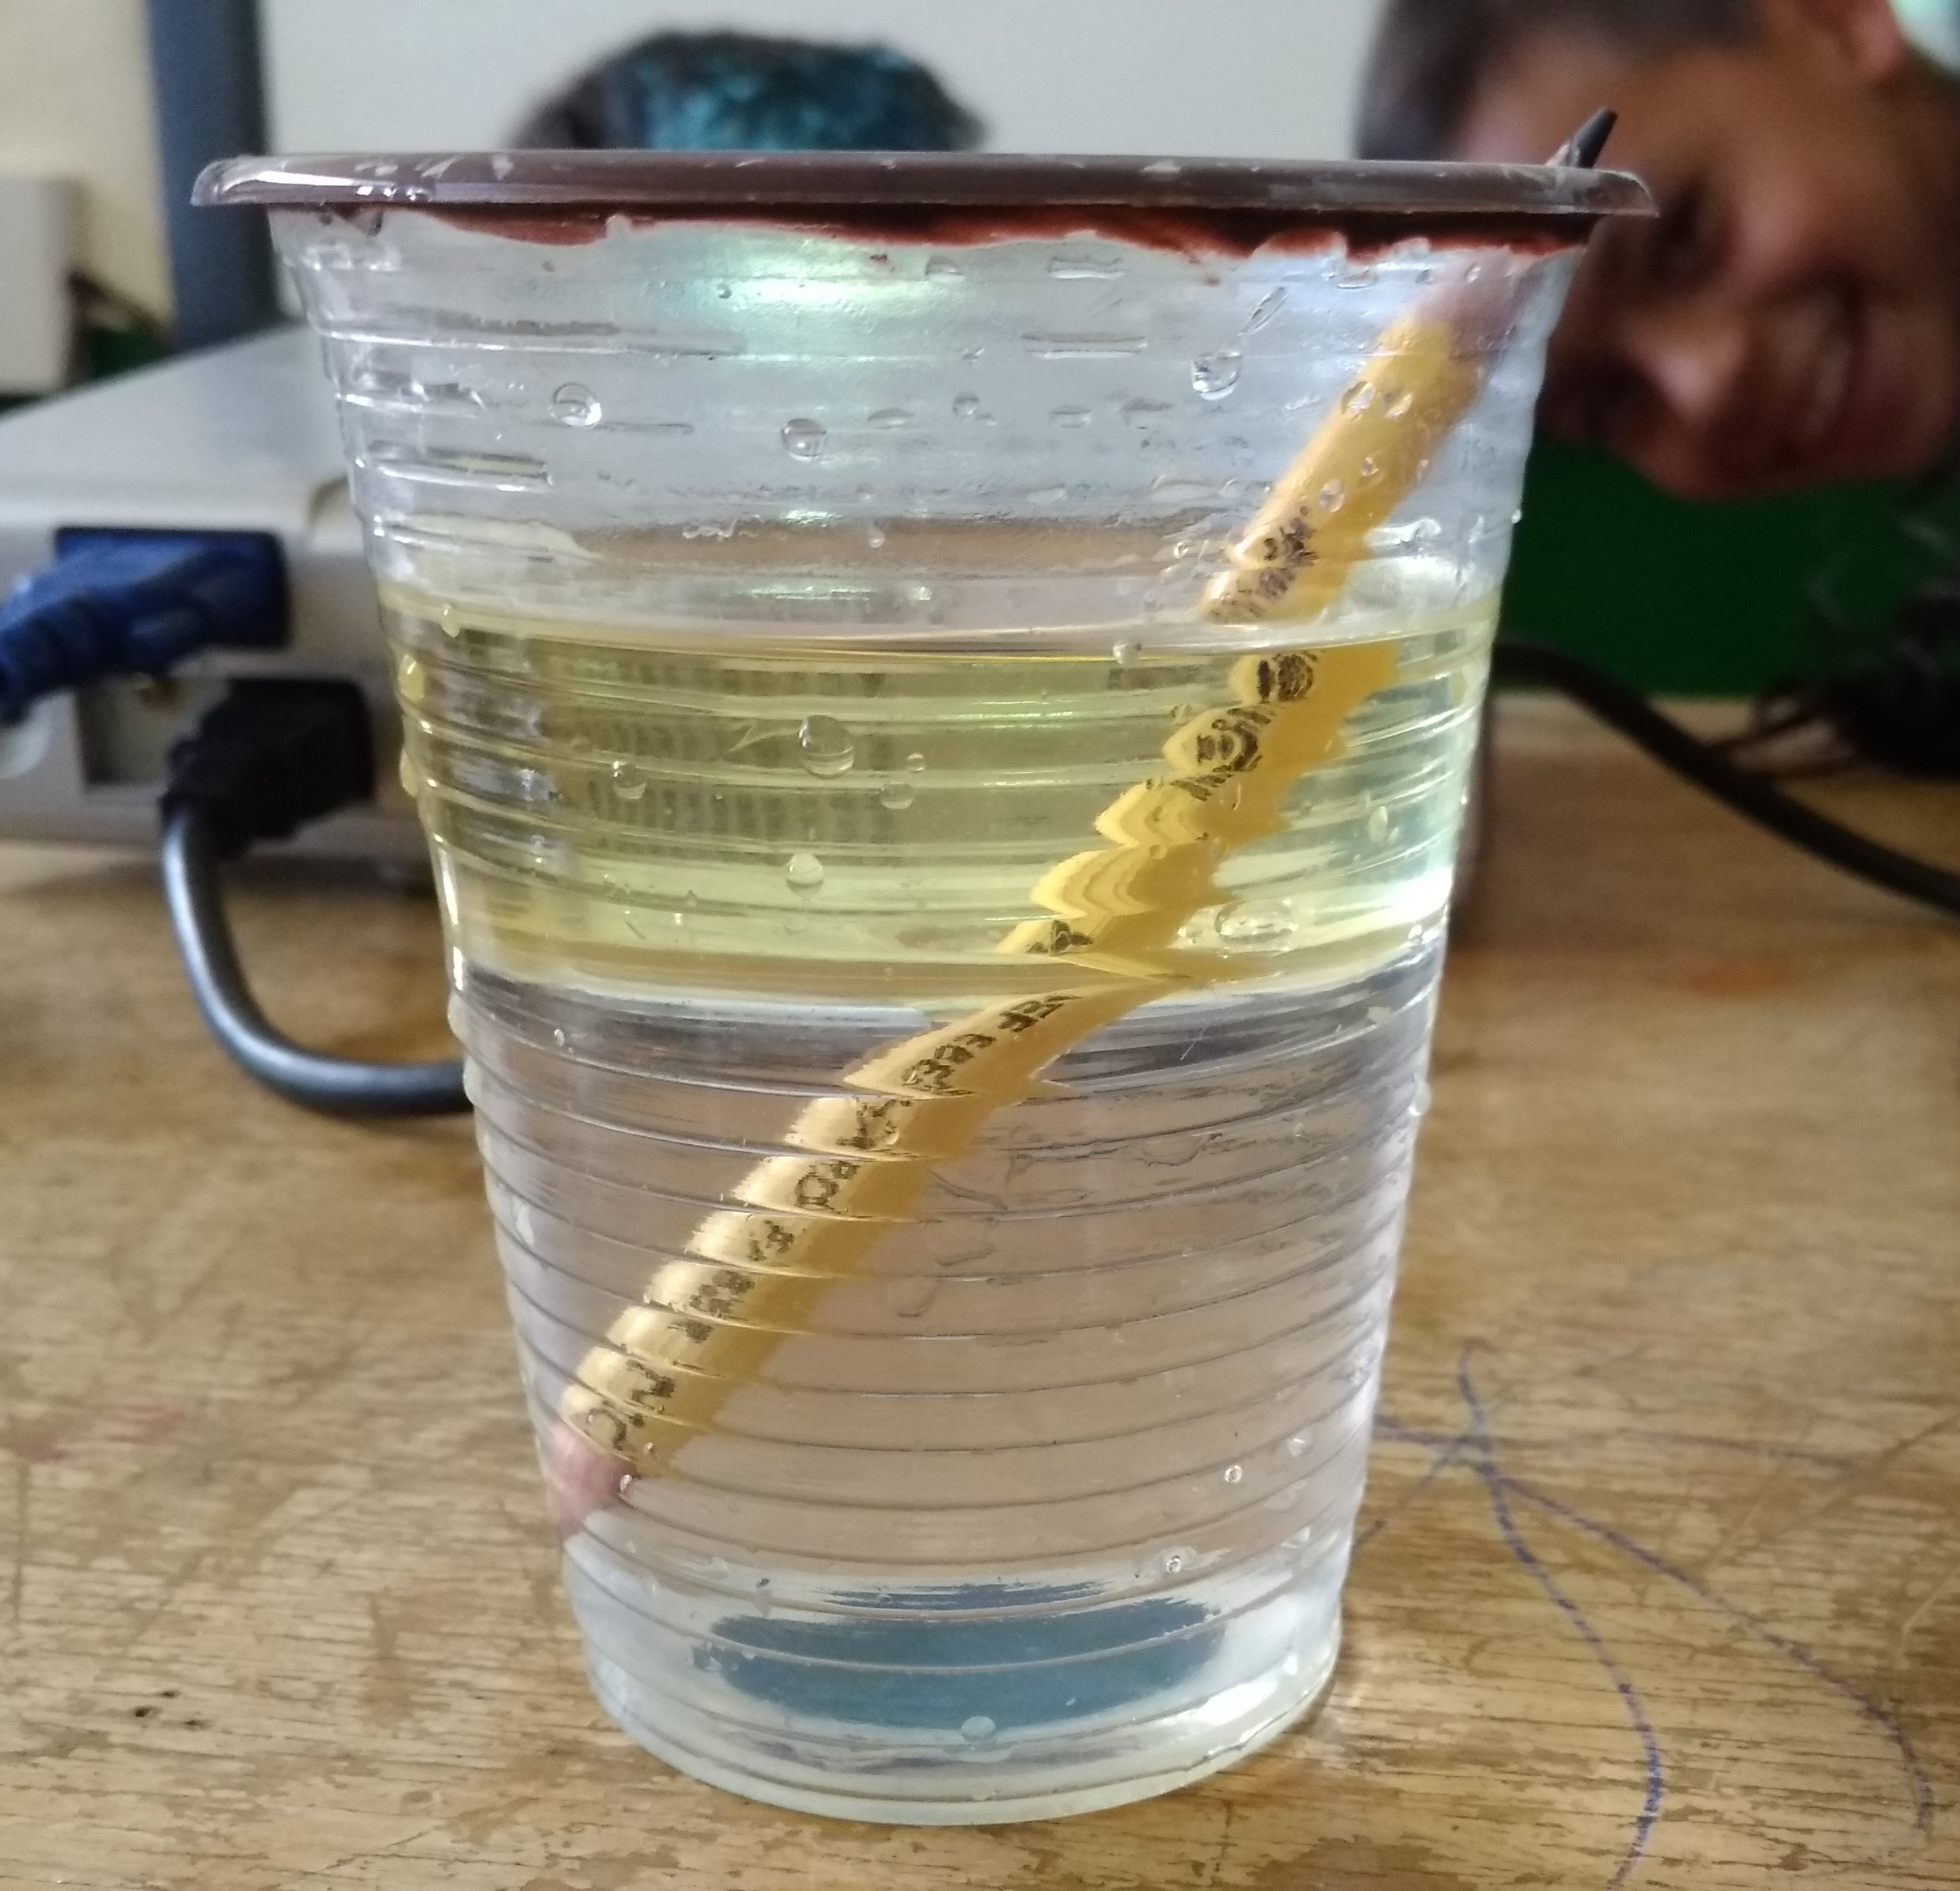
\includegraphics[height=5cm]{Imagenes/lapiz.jpg}
    \caption{Reflexión y refracción de la luz usando un láser y una lente en las Instituciones Educativas El Pórtico (izquierda) y Clavellinas (centro); y fenómeno de refracción de la luz en un lápiz en Clavellinas (derecha).}
\end{figure}


\noindent También se realizó el estudio de la polarización de la luz. Los estudiantes adquirieron el conocimiento del comportamiento del campo electromagnético. Se mostró el uso de la polarización en aplicaciones de la vida cotidiana. Por ejemplo, se realizó la demostración con el uso de las pantallas de dispositivos electrónicos y con lentes polarizadas.\\

\noindent Finalmente, se habló del fenómeno de difracción, en esta sección los estudiantes tuvieron la oportunidad de observar el fenómeno de difracción de la luz de un láser al pasar por una rejilla de difracción y al atravesar un cabello. También se hizo uso de gafas de difracción, con las cuales los estudiantes pudieron observar la composición espectral de la luz blanca. Especialmente con el uso del cabello, se pretendía explicar que la luz tiene un comportamiento diferente cuando se enfrenta a obstáculos pequeños y se hace la analogía con las ondas en el agua cuando atraviesan un agujero pequeño. Abordada la totalidad de los contenidos se dio por terminada la sesión.

\begin{figure}[H]
    \centering
    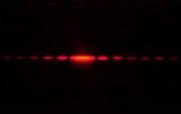
\includegraphics[width=7.5cm]{Imagenes/cabello.jpg}
    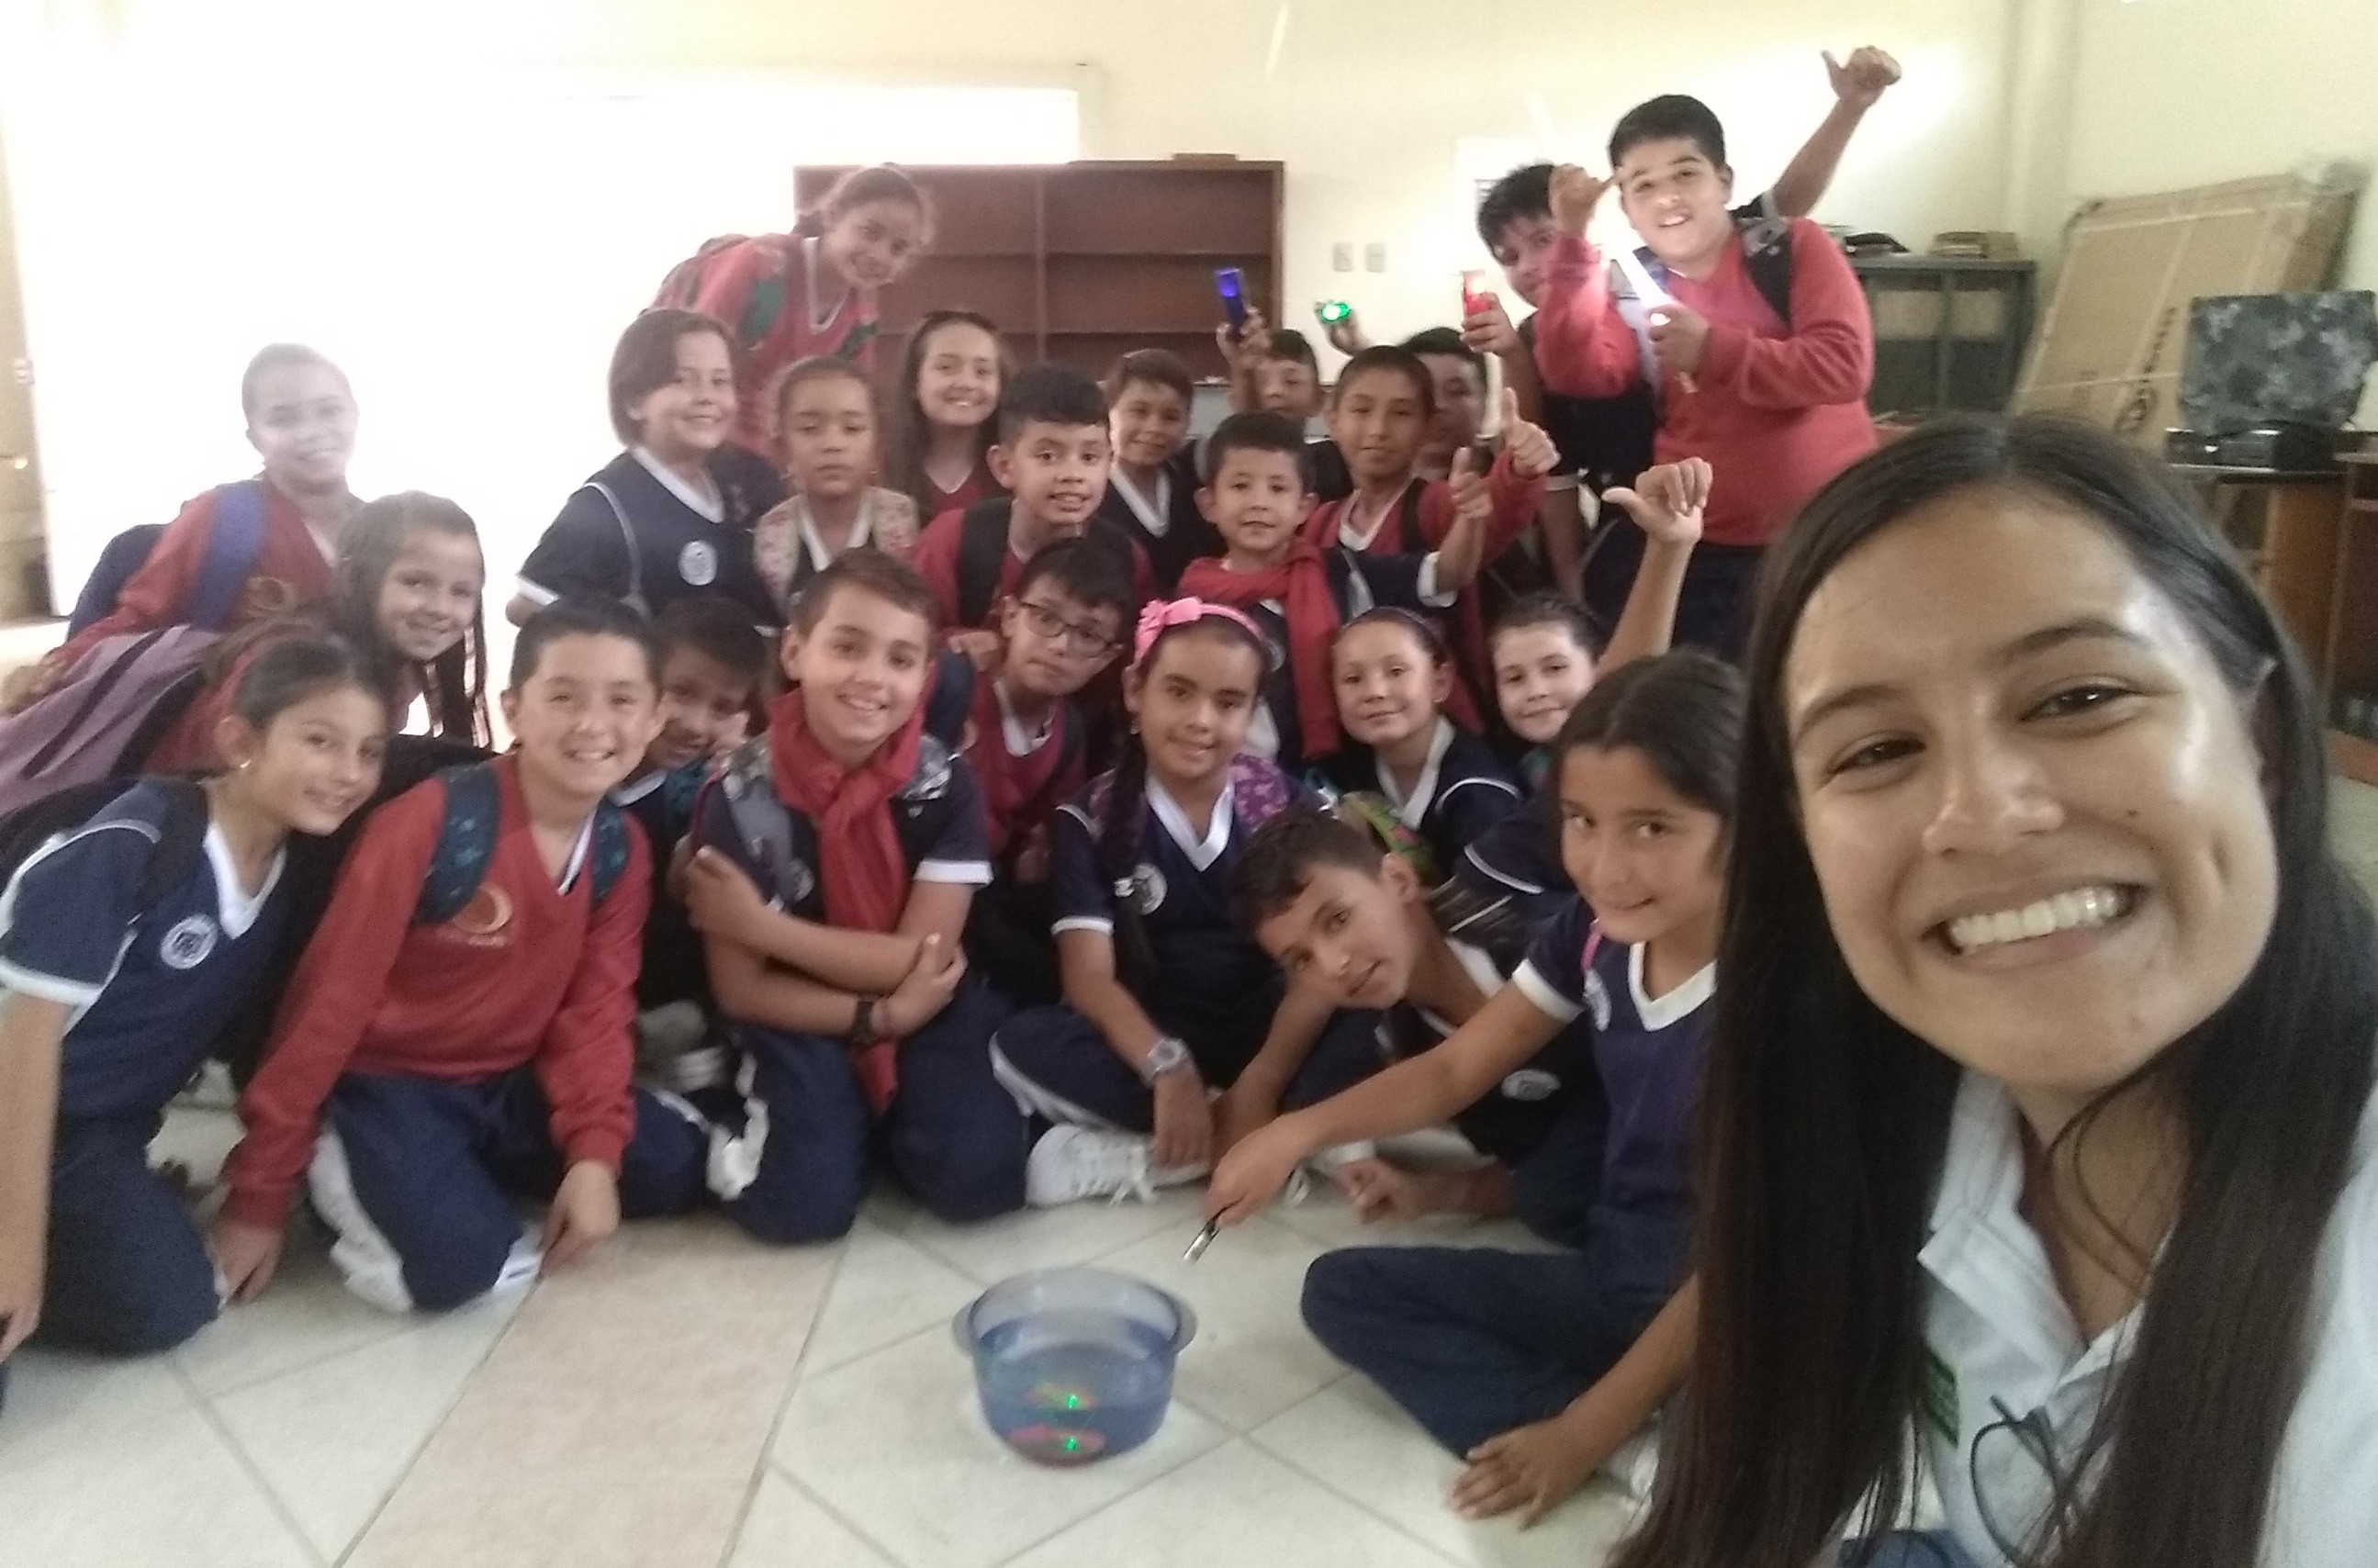
\includegraphics[width=7.5cm]{Imagenes/sanluis.jpg}
    \caption{Fenómeno de difracción usando un cabello, experimento realizado en la Institución Educativa Clavellinas (izquierda) y grupo de primaria grados cuarto y quinto al finalizar la actividad (derecha).}
\end{figure}
%-----------------------------------------------------------------------------------------

\section{Sistema Solar, exoplanetas y telescopios.}

\noindent En este bloque de trabajo se abordaron diferentes conceptos  los cuales fueron soportados en actividades didácticas de las siguientes temáticas:


\begin{figure}[H]
    \centering
    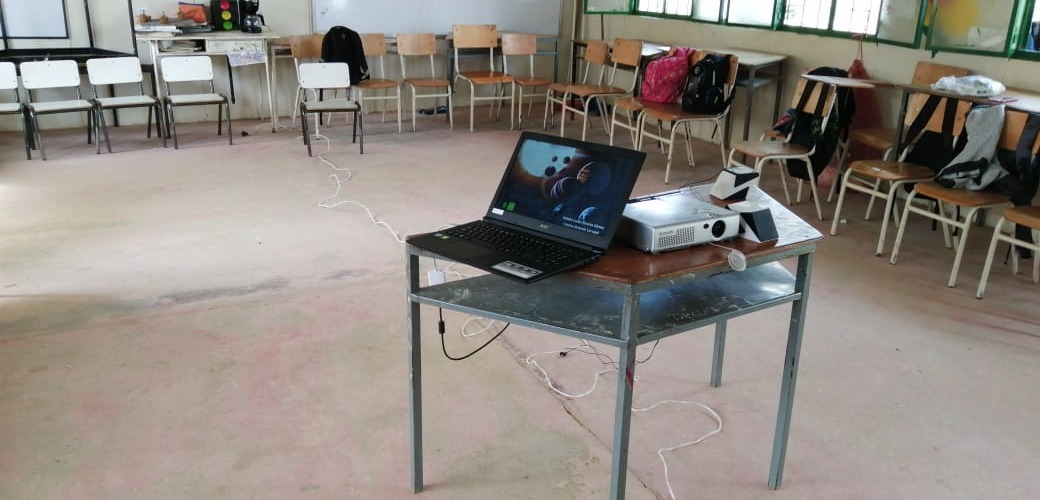
\includegraphics[width=10cm]{clavellinas/clave2.jpeg}
    \caption{Preparación de las actividades en la Institución Educativa Clavellinas.}
    \label{fig:my_label}
\end{figure}
\begin{itemize}
    \item ¿Qué es el sistema solar?
    \item El Sol, la estrella más cercana
    \item Formación estelar
    \item Planetas del sistema solar
    \item Relaciones de tamaños y distancias
    \item Exoplanetas y aliens
    \item Zona de habitabilidad
    \item Introducción al uso de telescopios
\end{itemize}

\
\subsection{Actividades desarrolladas}

\noindent \textbf{Formación estelar y del sistema solar (35 minutos)}
\vspace{2mm}

\noindent Para este primer acercamiento, es necesario tener en cuenta los pre-saberes de los estudiantes, para tener un punto del cual partir con las explicaciones en el resto de la sesión, por lo tanto se escucha los conocimientos de los estudiantes con respecto al tema del sistema solar. Posteriormente, se procede a dar una explicación introductoria, no solo de cómo se formó y evolucionó el sistema solar, sino también los primeros comienzos del universo, de manera consisa y sencilla, esto para la introducción de la formación estelar, e implementando ayudas audiovisuales para mayor comprensión.

\vspace{2mm}

\noindent \textbf{El sol, la estrella más cercana (35 minutos)}
\vspace{2mm}

\noindent Luego de introducir los tópicos importantes del punto anterior, se hizo un acercamiento a los cuerpos importantes del sistema solar, el primero de ellos el sol, el motor de la vida en la tierra y la estrella más cercana. Para abordar esta temática se introdujeron puntos importantes para entender las características, las funciones y la importancia de esta estrella. Además, se habló de futuro del sol y los drásticos cambios que conlleva en el nuestro sistema planetario. Finalmente, se mencionó la interacción con los demás cuerpos y en detalle con la Tierra. 

\vspace{2mm}

\noindent \textbf{Planetas y cuerpos del sistema solar (135 minutos)}

\vspace{2mm}

\noindent Luego de aprender respecto al astro rey, el Sol, se estudia el orden de los planetas en el sistema solar, las características específicas de cada uno de ellos y otros cuerpos celestes, como los asteroides y cometas. Para cada uno de ellos, se realizan diferentes actividades. 

\vspace{2mm}

\noindent Para el caso de \textit{Mercurio} se hace énfasis en su diferencia de rotación y traslación. En \textit{Venus}, se habla del efecto invernadero y se aprovecha el espacio para compartir con los estudiantes la importancia de cuidar el medio ambiente y evitar el calentamiento global, también se nombran sus fases, similares a las de la luna. Para la \textit{Tierra} se habla de la evolución, hechos importantes, tecnología, entre otros, al igual que para la \textit{Luna} se hace énfasis en el alunizaje, las fases y los cráteres, los cuales se pueden simular con harina y chocolate. En  \textit{Marte} se hace la comparación con la tierra y una actividad con imágenes que las compara, al igual de los hallazgos de agua en su superficie. Llegas a ese punto se abordan los cuerpos que guardan los secretos del inicio del sistema solar, los cometas y asteroides, aquí se mencionan las diferencias entre ellos, la forma de las órbitas, y los componentes de cada uno de estos, enfatizando significativamente en los cometas y su capa de agua congelada, para esto se desarrolló una actividad donde, con materiales sencillos, se hizo un cometa.\\

\begin{figure}[H]
    \centering
    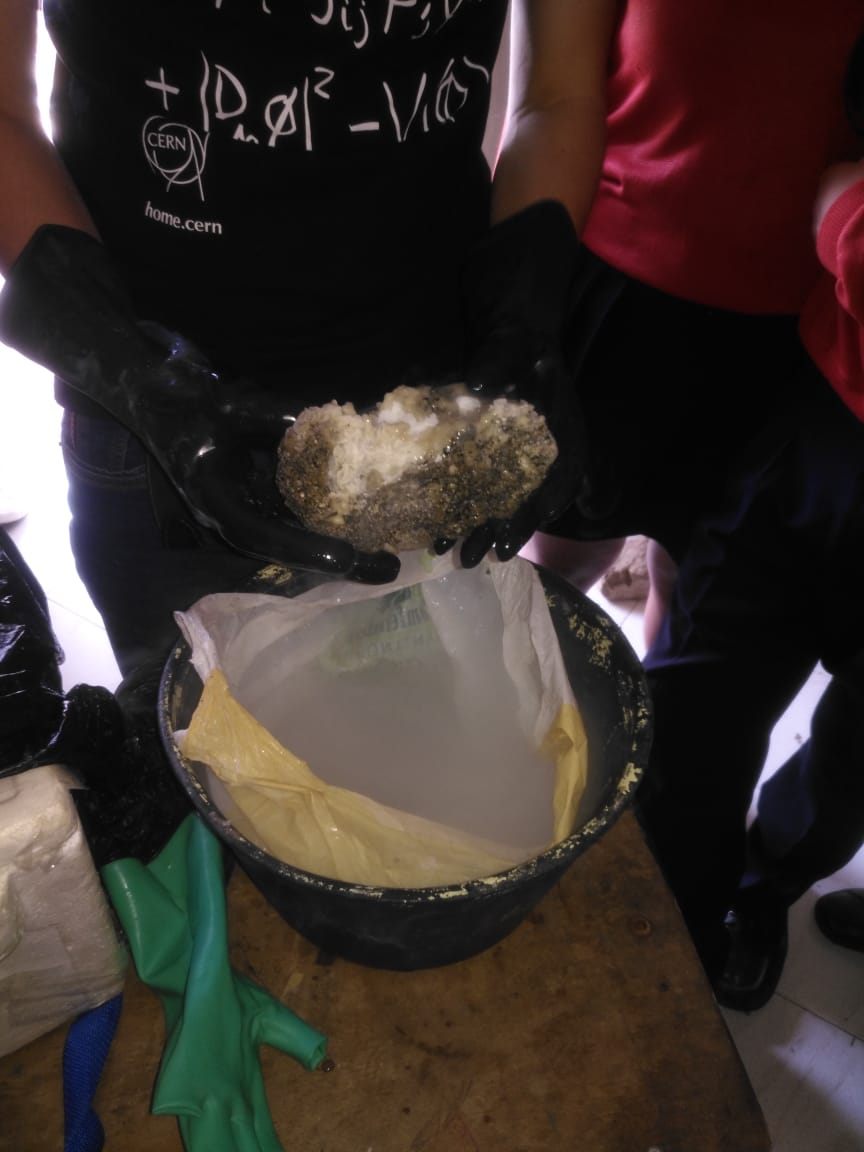
\includegraphics[width=4cm]{clavellinas/cometa11.jpeg}
    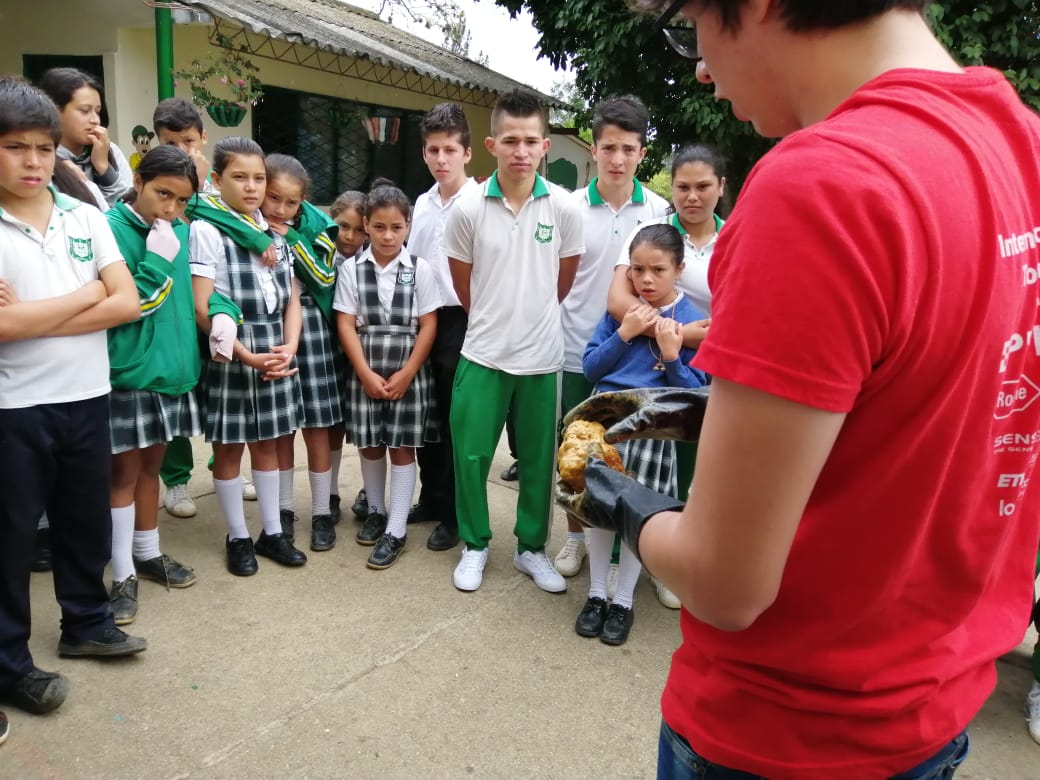
\includegraphics[width=7.9cm]{clavellinas/cometa2-portico.jpeg}
    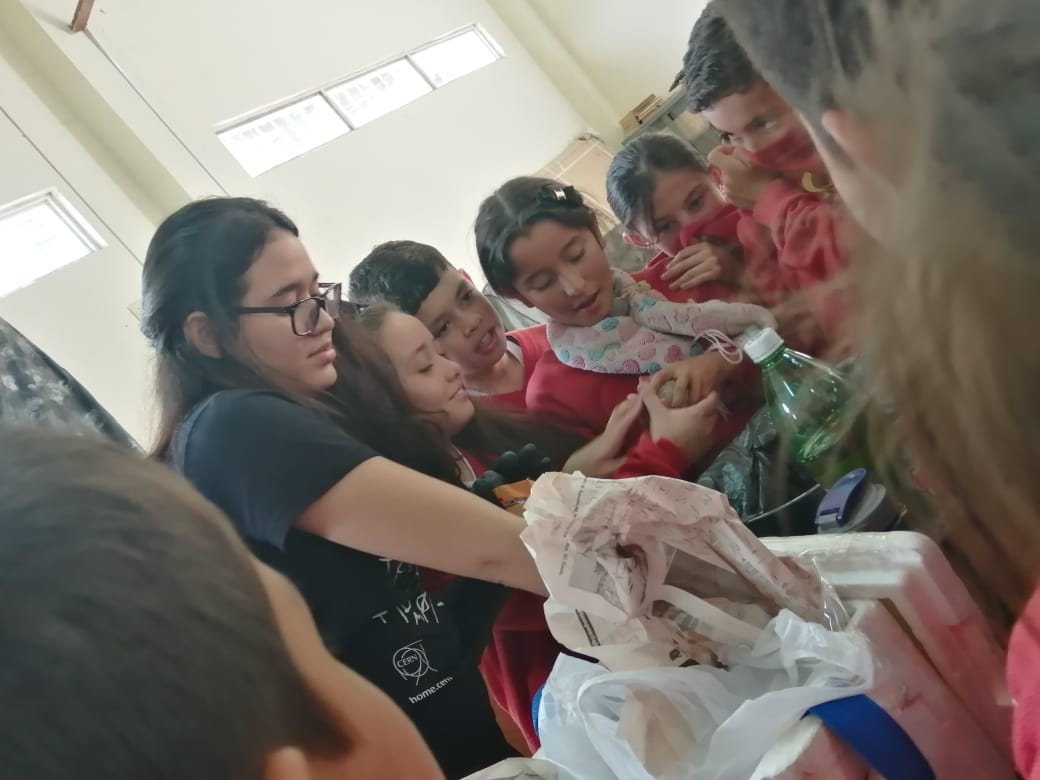
\includegraphics[width=5.95cm]{clavellinas/cometa-sanluis.jpeg}
    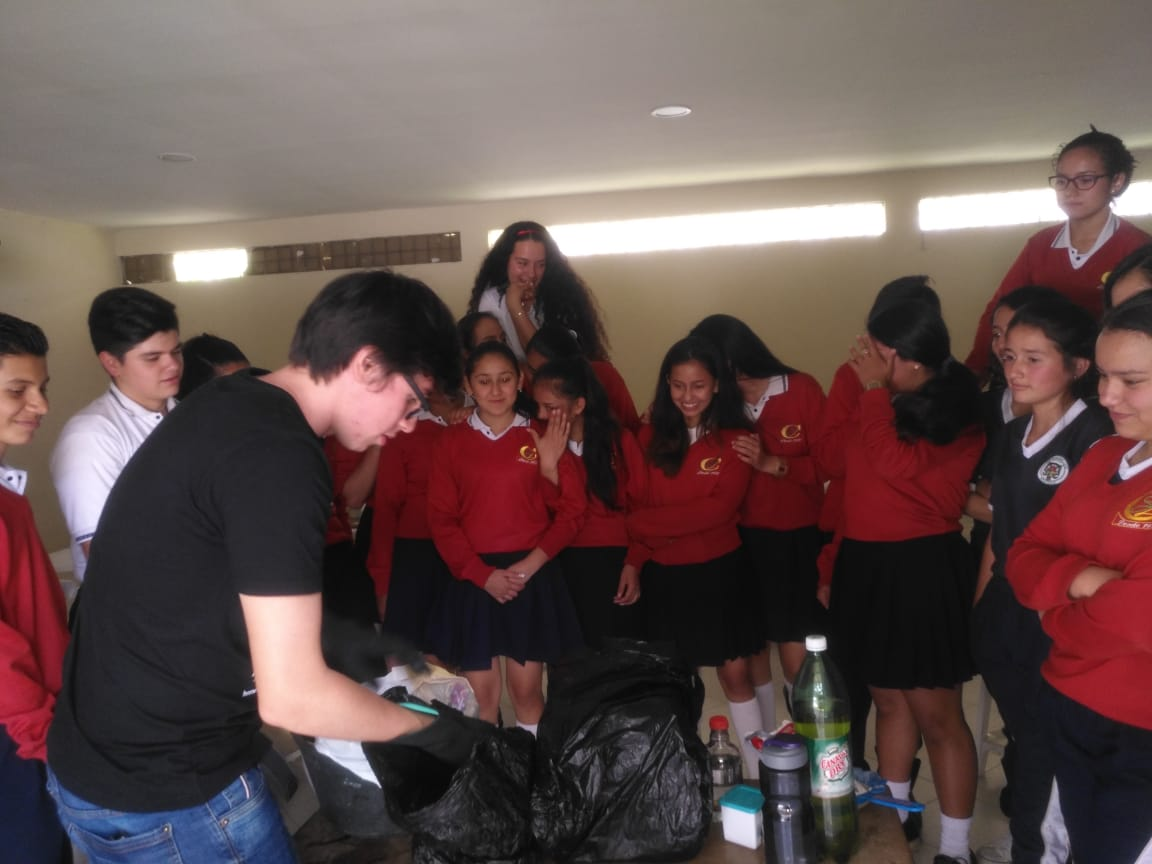
\includegraphics[width=5.95cm]{clavellinas/cometa-sanluiss.jpeg}
    \caption{Actividad de la formación del cometa realizada con los estudiantes en el marco del Sistema Solar.}
    \label{fig:my_label}
\end{figure}

\noindent En \textit{Júpiter} se hace referencia a su gran tamaño, sus lunas y tormentas; En \textit{Saturno}, a sus grandes anillos y auroras boreales; Con estos dos últimos se realizaron actividades de achatamiento de polos con ayuda de cartulinas y palos de pincho. 

\begin{figure}[H]
    \centering
    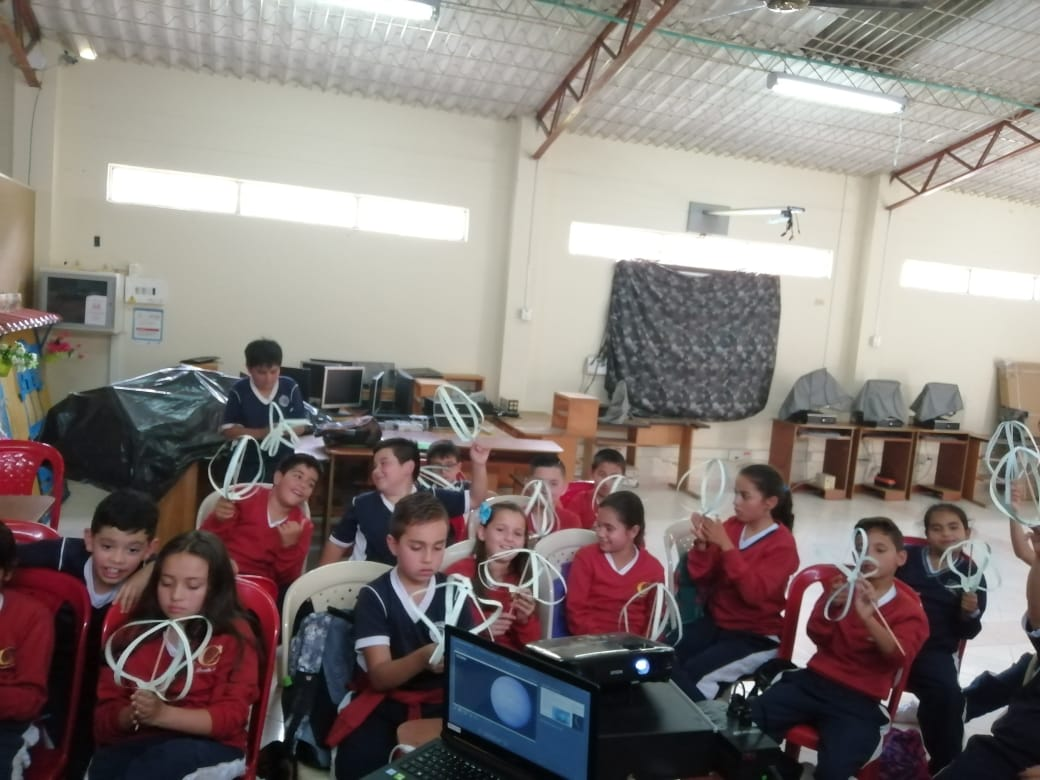
\includegraphics[width=9cm]{clavellinas/sanluis-achatamiento.jpeg}
    \caption{Actividad de achatamiento de los planetas.}
    \label{fig:my_label}
\end{figure}

\noindent Para los dos últimos planetas del Sistema Solar se trata solo la parte teórica y se hace la explicación de por qué \textit{Plutón} ya no es un planeta.

\vspace{2mm}

\noindent \textbf{Relaciones de tamaños y distancias (45 minutos)}

\vspace{2mm}

\noindent La inmensidad del sistema solar y en general de las distancias astronómicas no son realmente dimensionadas cuando se quedan simplemente en los millones de kilómetros, por ende es necesario recurrir a actividades que las vuelva palpables. Para comprender las grandes diferencias de los tamaños de los cuerpos de nuestro sistema planetario, que van desde miles de miles hasta millones de kilómetros, se hizo un escalamiento de los diámetros de los planetas junto con el sol hasta lograr considerar y magnificar el diminuto tamaño de la tierra contra los grandes planetas y contra la inmensa estrella. La actividad correspondiente a las distancias entre los cuerpos planetarios y el sol, se hizo mediante una cinta de papel donde se marcaron las distancias escalas de cada uno de los cuerpos, aquí se pudo visualizar que la Tierra realmente está a una diminuta distancia del sol, en comparación con Neptuno el planeta más distante.    


\begin{figure}[H]
    \centering
    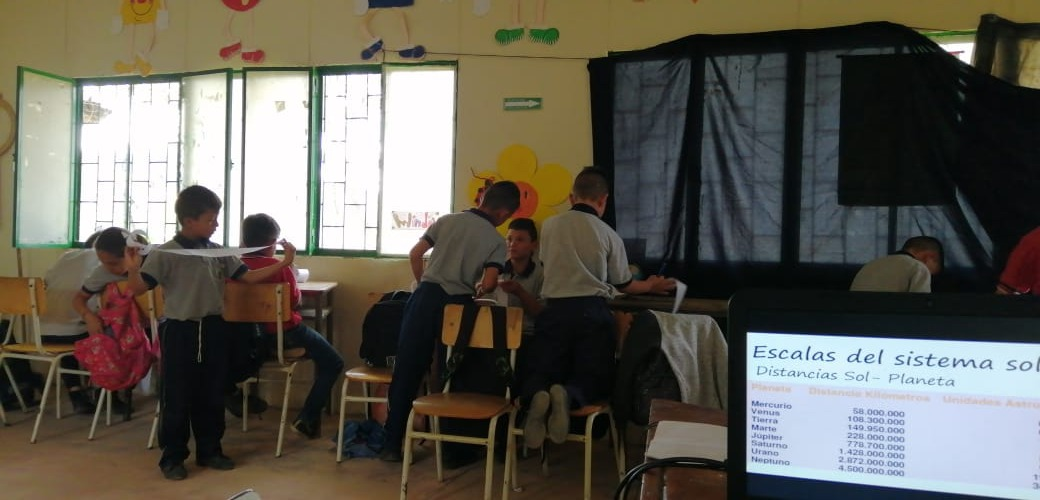
\includegraphics[width=8cm]{clavellinas/clave.jpeg}
    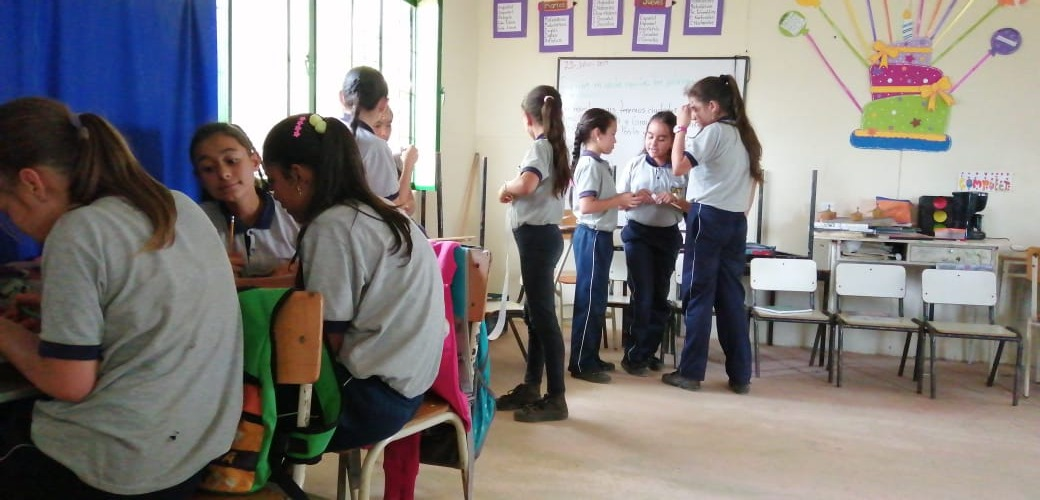
\includegraphics[width=8cm]{clavellinas/clave1.jpeg}
    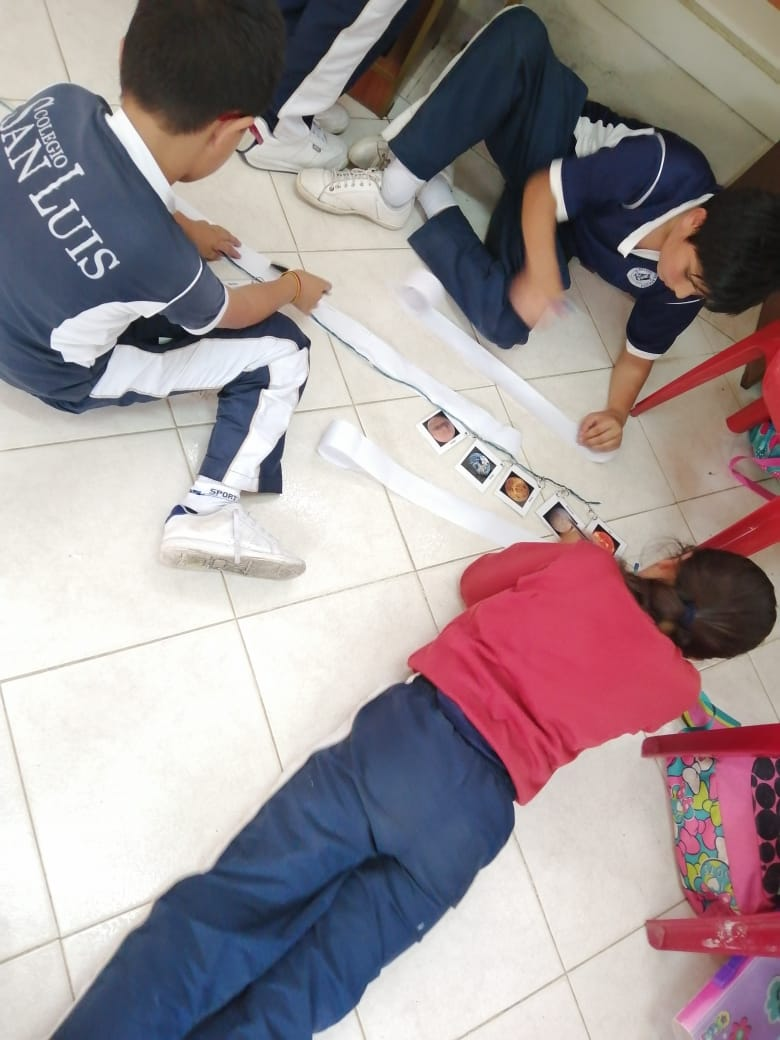
\includegraphics[width=8cm]{clavellinas/distancias-sanluis.jpeg}
    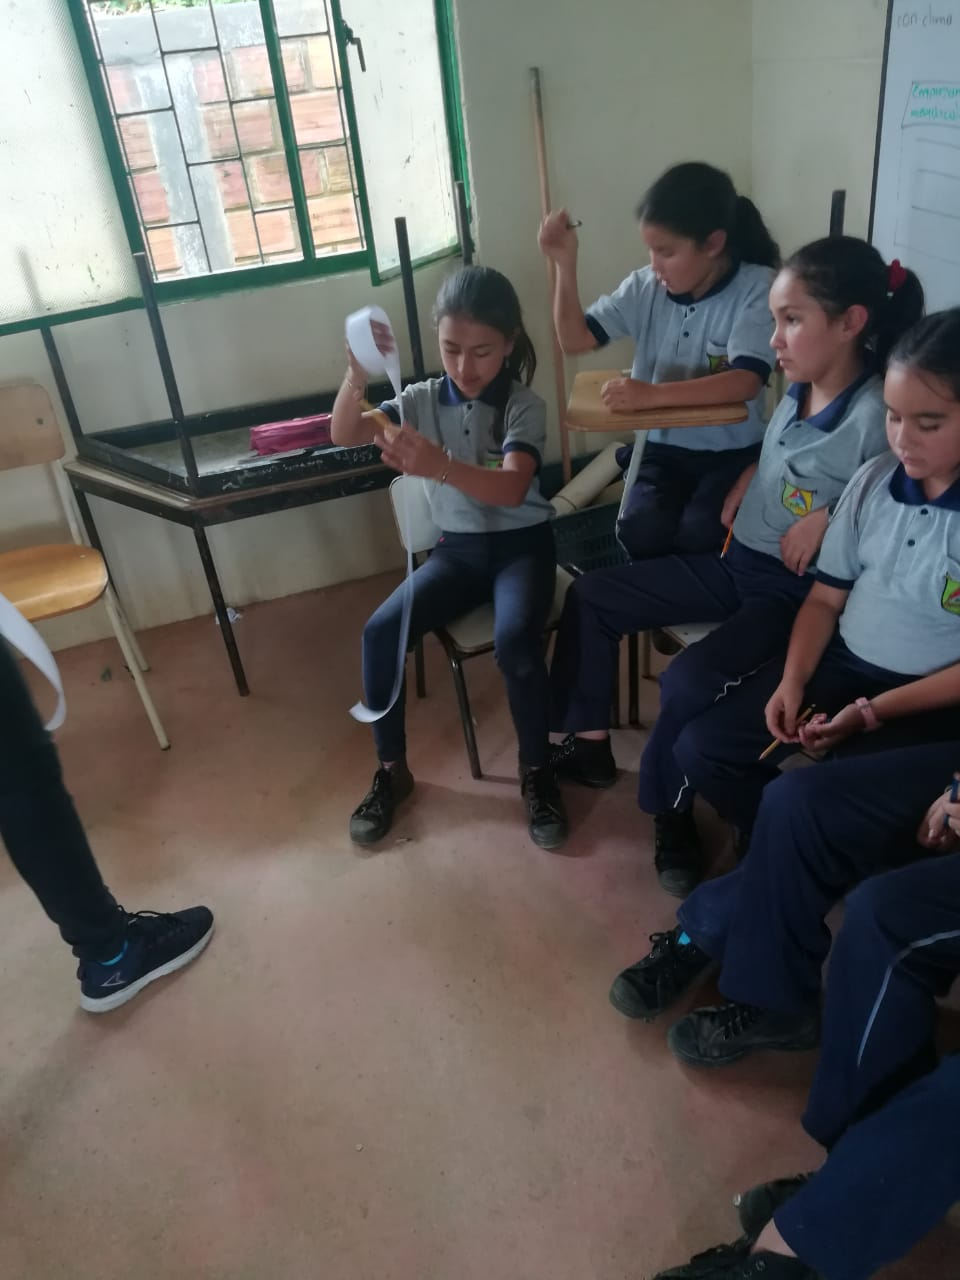
\includegraphics[width=8cm]{clavellinas/clavellinas-dist.jpeg}
    \caption{Estudiantes participando en la actividad de relación de distancias.}
\end{figure}

\begin{figure}[H]
    \centering
    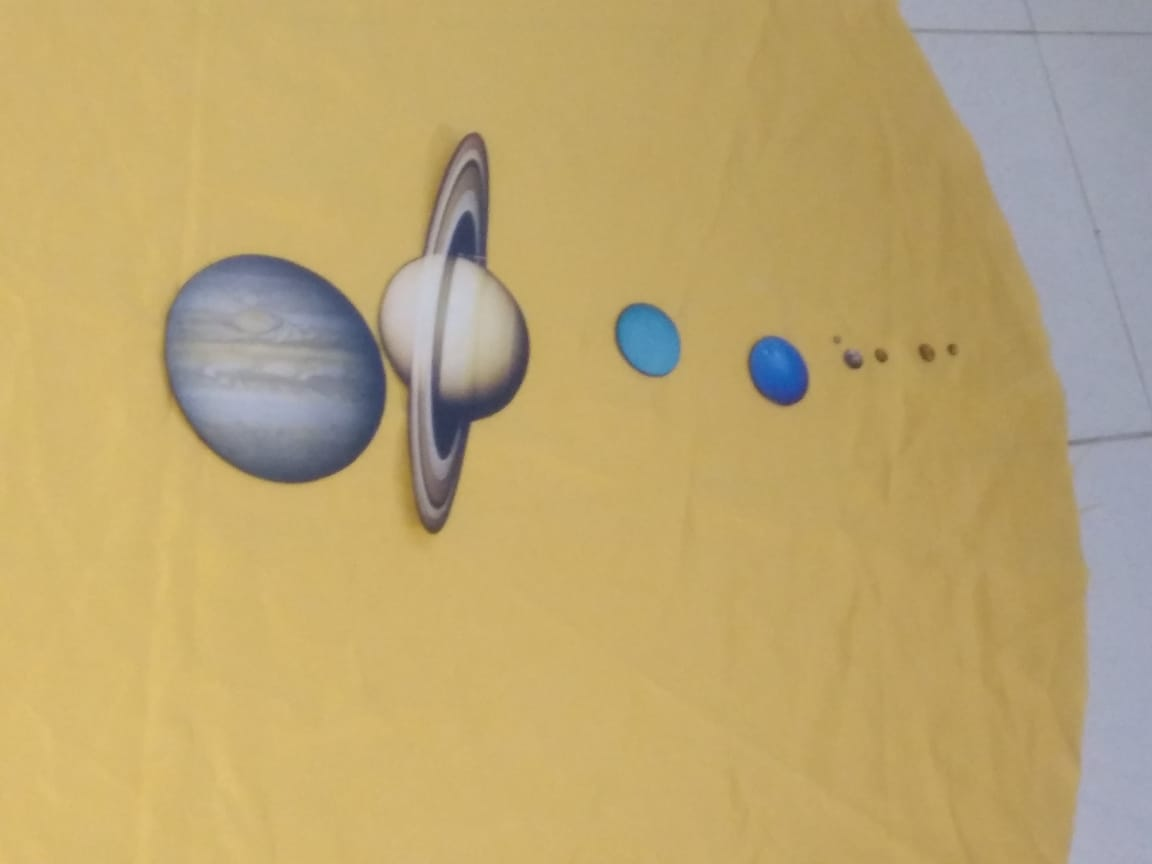
\includegraphics[width=10.6cm]{clavellinas/tamanos.jpeg}
    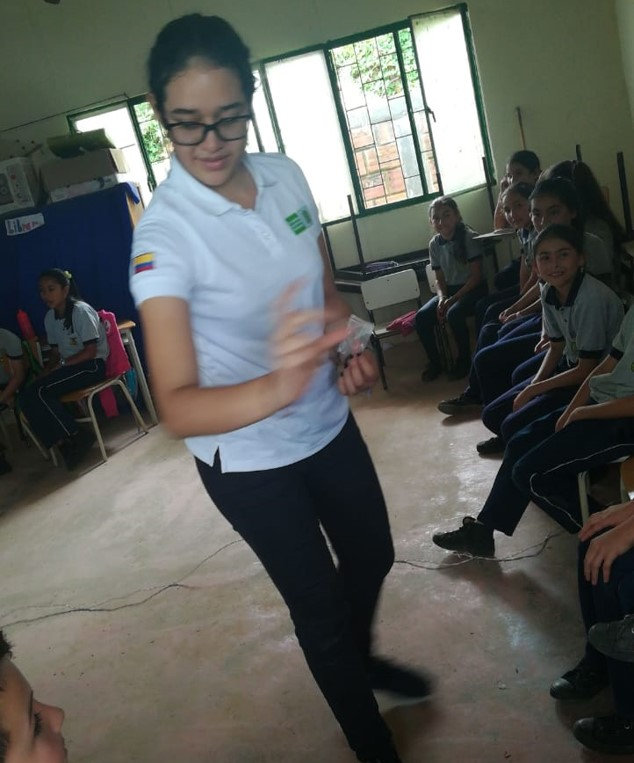
\includegraphics[width=6.6cm]{clavellinas/tamanos-1.jpg}
    \caption{Realización de la actividad de relación de tamaños.}
\end{figure}



\vspace{2mm}


\noindent \textbf{Exoplanetas y zona de habitabilidad (30 minutos)}

\vspace{2mm}

\noindent Más allá de los confines de nuestro sistema se encuentran una gran cantidad de mundos y de millones de estrellas con planetas en órbitas, que forman sistemas extraplanetarios similares al sistema solar. La búsqueda de estos exoplanetas no es tarea fácil, se necesita recurrir a diversas técnicas muy precisas para lograr detectarlos. Mediante simulaciones, vídeos y discusiones se establecieron los conceptos necesarios para estudiar y comprender las diferencias de estos sistemas y planetas con relación al nuestro, además se discutieron las técnicas de detección y se habló de una características fundamental para la posible existencia de la vida, la zona de habitabilidad. Esta relaciona la distancia de la estrella a los planetas y el tamaño de esta para configurar la posibilidad de que el planeta en cuestión albergue agua líquida.



\vspace{2mm}

\noindent \textbf{Introducción al uso de telescopios (20 minutos)}

\vspace{2mm}

\noindent Por último se estudian los diferentes tipos de instrumentos que se implementan para el estudio de cuerpos celestes, para ello se ahonda en sus partes, en cómo pasa la luz a través de ellos para reconstruir las imágenes que nos brinda la información de los cuerpos, también se habla de los primeros y los últimos telescopios, además de los inicios de la óptica y la importancia en estos instrumentos. Esta sección se empalma con la jornada de observación solar. 


\begin{figure}[H]
    \centering
    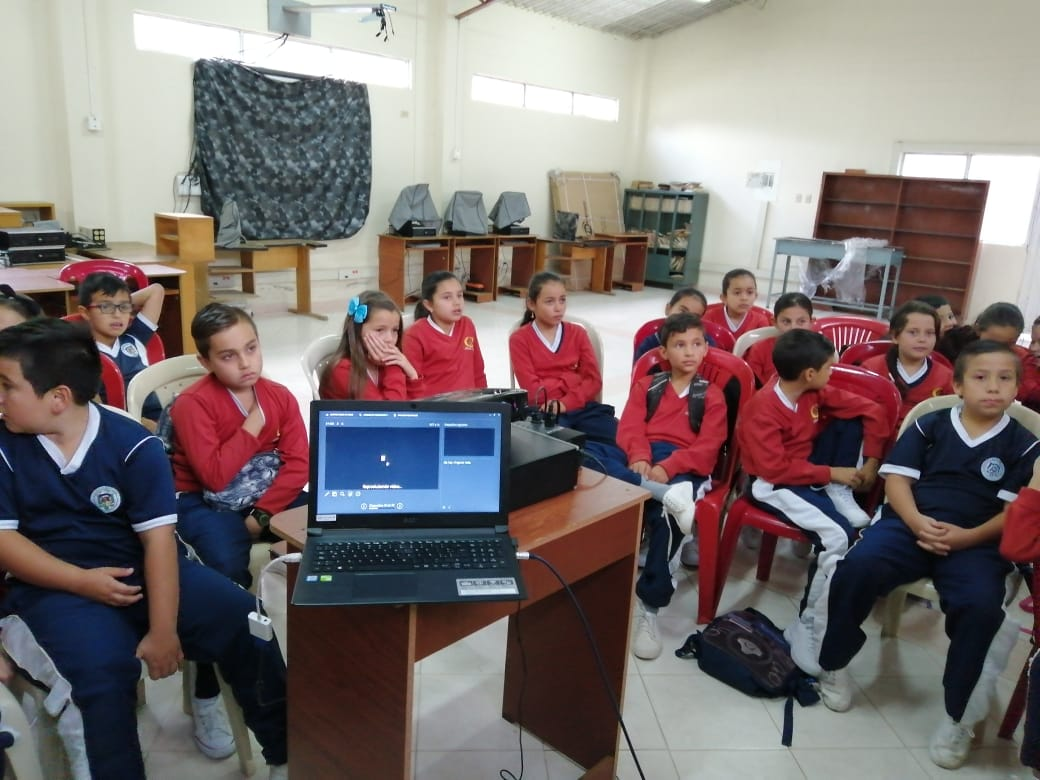
\includegraphics[width=8.5cm]{clavellinas/sanluis-exp.jpeg}
    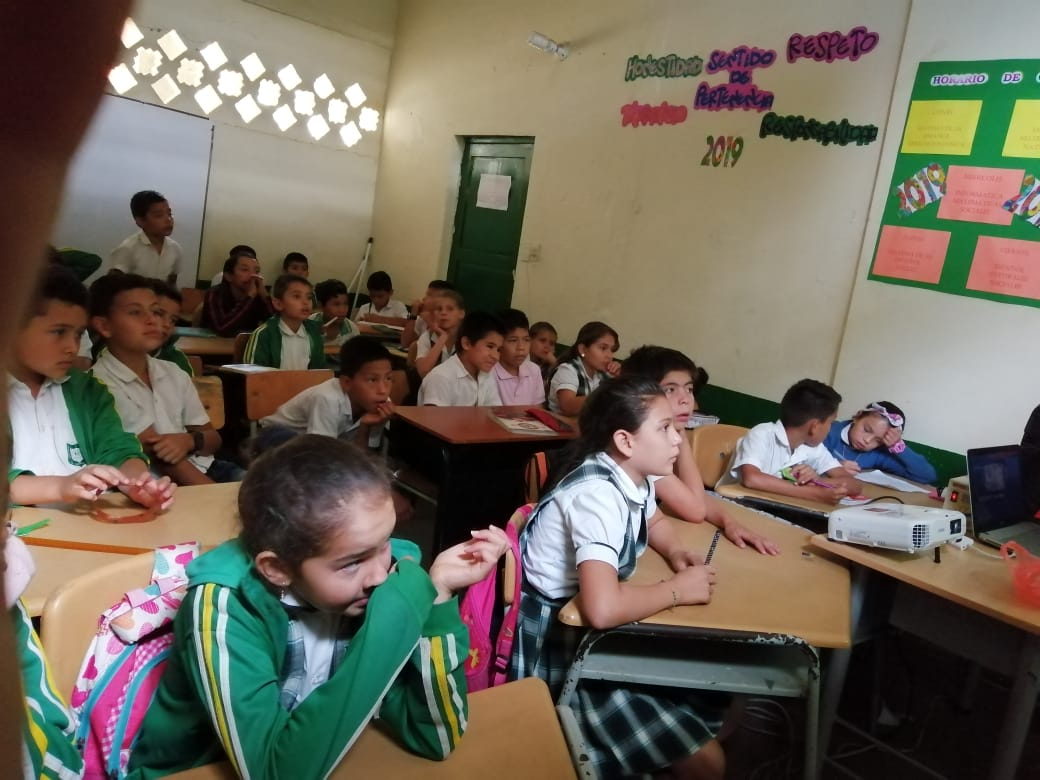
\includegraphics[width=8.5cm]{clavellinas/portico.jpeg}
    \caption{Realización de la actividad de relación de tamaños.}
\end{figure}

\noindent Al final de la jornada, se le pidió a los niños que realizaran composiciones artísticas, como dibujos o pequeñas maquetas de lo que más les había gustado de la sesión de trabajo, los resultados son muy enriquecedores y reflejan el gran trabajo realizado.


\begin{figure}[H]
    \centering
    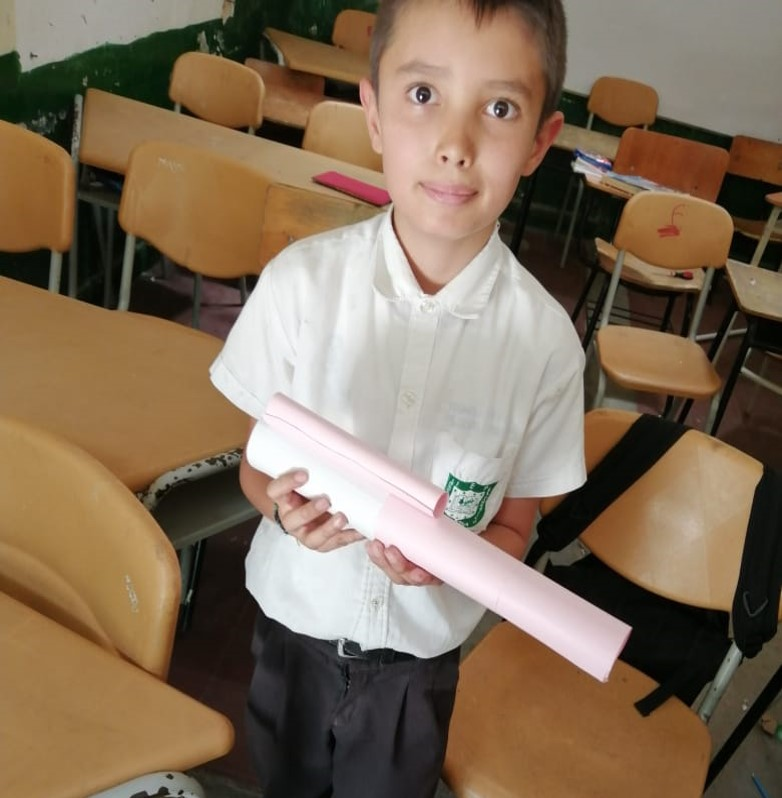
\includegraphics[width=6.35cm]{clavellinas/Imagen1.jpg}
    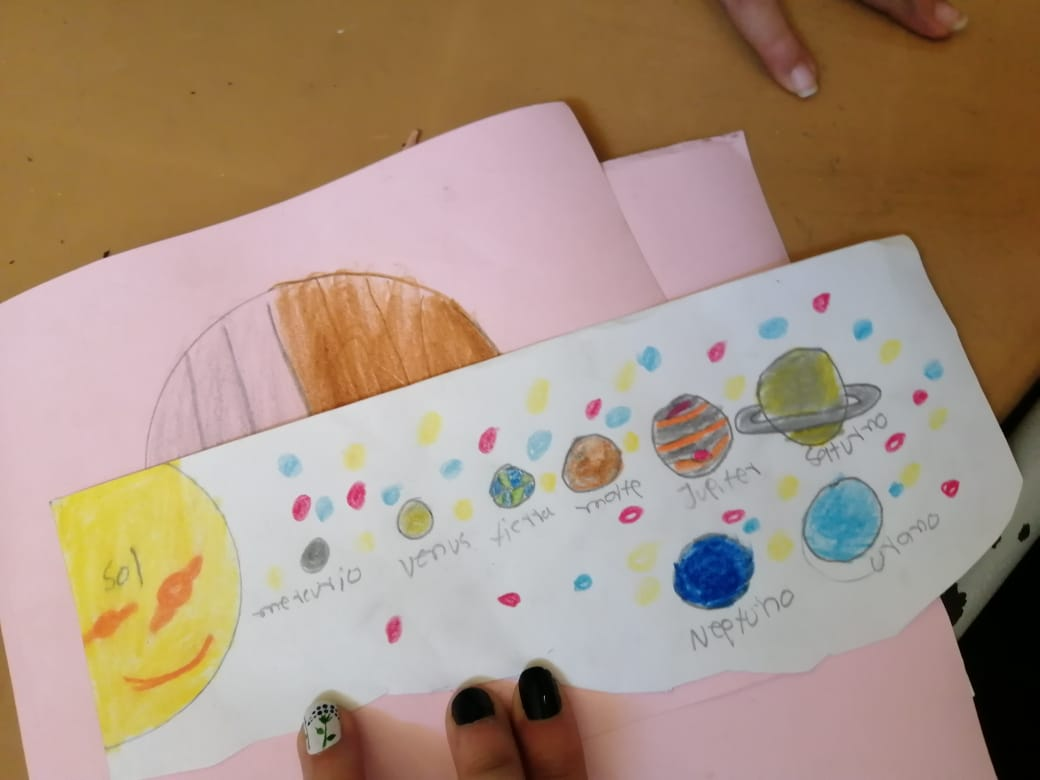
\includegraphics[width=8cm]{clavellinas/act-sistsolar.jpeg}
    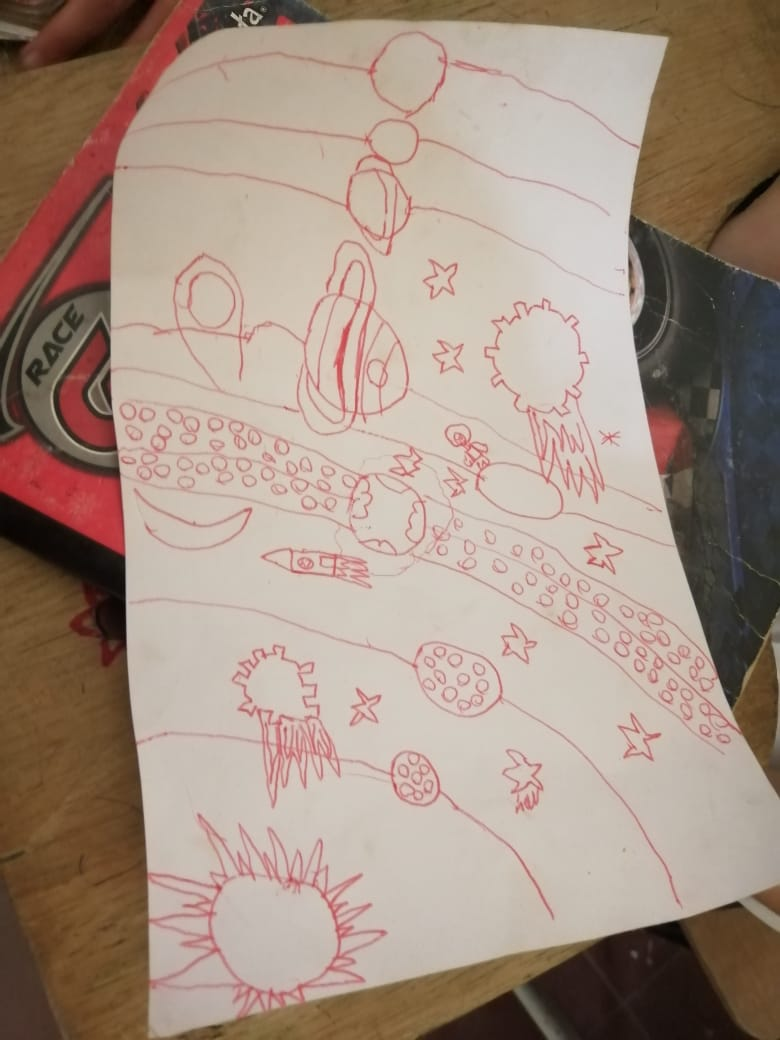
\includegraphics[width=5.5cm]{clavellinas/act-sistsolar1.jpeg}
    \includegraphics[width=5.5cm]{clavellinas/act-sistsolar2.jpeg}
    \caption{Realización de la actividad de relación de tamaños.}
\end{figure}

\section{Sistema local Sol-Tierra-Luna }

\noindent En el presente bloque de actividades, los estudiantes son separados en dos grupos cuyos integrantes son por un lado los grados menores (cuarto y quinto) y por otro los grados mayores (noveno y décimo). En este caso los instructores realizan rotaciones de manera que ambos puedan desarrollar la mitad de la jornada con cada uno de los grupos. La temática a tratar se dividió en los siguientes tópicos:

\begin{itemize}
    \item Bóveda celeste

    \item El sol (manchas solares)

    \item Viajes espaciales

    \item Práctica: Jornada de observación diurna.

    \item La luna y su estructura geológica

    \item Movimientos relativos entre el Sol, la Tierra y la Luna
    
    \item Los eclipses
    
    \item Práctica: Cohetería
    
\end{itemize}


\noindent Las actividades presentadas fueron dictadas en el orden ya mostrado con el fin de seguir una línea lógica de pensamiento y crear una guía de ideas clara y coherente. 

\subsection{Actividades desarrolladas}


\noindent \textbf{Bóveda celeste (40 minutos)}\\

\noindent Para esta temática se realizó una actividad introductoria con el fin de caracterizar los conocimientos previos del grupo de estudiantes, para ello se les solicitó que dibujaran en una hoja de papel todo lo que ellos considerasen que formaba parte del cielo. Acto seguido se socializaron las ideas comunes y se les presentó el concepto de bóveda celeste en propiedad. Haciendo uso del software libre de simulación estelar: 'Stellarium', se permitió a los estudiantes explorar toda la bóveda celeste para identificar constelaciones, satélites, estrellas, galaxias y planetas, consolidándose las ideas previamente presentadas, para finalizar la actividad con la construcción de una carta celeste por parte de cada alumno.\\

\begin{figure}[H]
    \centering
    \includegraphics[width=10cm]{J-S/Bc.jpg}
    \caption{Colegio San Luis de Aratoca.}
    \label{fig: bovedaceleste}
\end{figure}

\noindent \textbf{El sol (manchas solares) (30 minutos)}\\

\noindent Esta práctica involucraba a los estudiantes de una manera diferente a todas las demás actividades presentadas previamente, puesto que estuvo diseñada con el objetivo de otorgar todos los conceptos necesarios previos a la realización de la práctica de observación diurna. Nuevamente se comenzó la actividad efectuando un sondeo de conceptos previos sobre el astro rey a través de una charla instructor-alumnado, acto seguido se realizó una presentación de la historia de la observación solar, para terminar con la introducción de conceptos claves de la formación estelar y las características generales de nuestro sol entre las cuales se le brindó especial atención a la explicación del fenómeno de manchas solares, con la esperanza de poder identificarlas en la realización de la observación diurna.\\

\noindent \textbf{Viajes espaciales (20 minutos)}\\

\noindent La construcción de conocimiento en torno a los viajes espaciales estuvo enfocada como una charla magistral en la que se habló de la historia de la exploración espacial por parte de la humanidad, aprovechando la conmemoración de los cincuenta años del viaje del hombre a la luna, para finalizar dando un recorrido por las principales misiones espaciales de la historia, haciendo énfasis en los dispositivos empleados para lograr estos objetivos: sondas espaciales, cohetes y rovers. Para finalizar esta sección se le solicitó al alumnado describir su viaje espacial soñado.\\

\noindent \textbf{Práctica: Jornada de observación diurna (60 minutos)}\\

\noindent Esta práctica metodológica estuvo totalmente enfocada en el aprendizaje a través de la acción, puesto que cada uno de los estudiantes tuvo la oportunidad de ver y manejar por completo un telescopio a través de la observación solar llevada a cabo. Cada alumno pudo aprender las características generales del armado y disposición de un telescopio para observación diurna, abonado a un tiempo extendido para realizar observación del astro rey. Mientras un estudiante visualizaba por el telescopio se les facilitó a los demás alumnos la posibilidad de emplear un catalejo con el objetivo de vislumbrar los objetos mas cercanos, como cumbres de montañas y paisaje general.\\

\begin{figure}[H]
    \centering
    \includegraphics[width=12cm]{J-S/solar.png}
    \caption{Colegio San Luis de Aratoca \textit{(Izquierda superior)}, Institución Educativa Clavellinas \textit{(Derecha superior) e Institución Educativa El Pórtico (izquierda y derecha inferiores)}}
    \label{fig: solar}
\end{figure}


\noindent \textbf{La luna y su estructura geológica (50 minutos)}\\


\noindent La actividad inicia con una dinámica de conversación entre los estudiantes y el tallerista sobre la pregunta planteada "¿Que es la astronomía?" y "¿Para qué es importante esta en la vida cotidiana?". Esto es fundamental para realizar un sondeo general del nivel de conocimiento actual en el curso. Posterior a esto se dio paso a una charla del instructor en la cual se explica brevemente el proceso de la formación del sistema solar, llegando a la formación del planeta tierra en específico, en donde acto seguido, y continuando con la línea de sistema Sol-Tierra-Luna, se le pidió a los estudiantes que formularan sus propias hipótesis de formación lunar. En este proceso, se les explicó qué es una hipótesis y cómo formularla. Las ideas presentadas por los mismos estudiantes fueron puestas en contraste con la teoría de formación principal (El gran impacto), involucrando en medio diferentes actividades físicas, como por ejemplo la rotación de un estudiante sobre su propio eje (Teoría de fisión), para ejemplificar las teorías planteadas por la comunidad científica. Nuevamente, con ayuda del VideoBeam, simulaciones científicamente fundamentadas fueron presentadas a los estudiantes, ahora para visualizar el proceso de formación de los cráteres lunares debido a la colisión de asteroides, dando así nuevamente un espacio de conversación hacia la propia geología lunar y los materiales (silicatos y metales) que la conforman.\\

%Los resultados obtenidos de esta conversación se resumen en que aunque los jóvenes mayores (9° y 10°). Aunque no poseían los conocimientos básicos conceptuales a total claridad, tenían una idea acertada del objeto de estudio de la astronomía y su función en la historia de la humanidad.

\begin{figure}[H]
    \centering
    \includegraphics[width=11cm]{J-S/luna.png}
    \caption{Colegio San Luis de Aratoca \textit{(Izquierda)}, Institución Educativa Clavellinas \textit{(Derecha).}}
    \label{fig: Luna}
\end{figure}


\noindent \textbf{Movimientos relativos entre el sol, la tierra y la luna (30 minutos)}\\

\noindent Posteriormente se sale del aula de clase a un espacio abierto, donde la temática del sistema Tierra-Sol-Luna puede ser tratado. Es este caso fue necesaria la ayuda de tres estudiantes (con los demás observando la actividad) en donde ellos mismos realizaban el complejo proceso de rotación y traslación del planeta tierra y su satélite natural al rededor del astro rey (el sol). Esta actividad es de vital importancia para comprender y dar claridad no solamente al fenómeno del día y la noche, sino también para la comprensión del transcurso de las estaciones del año (verano, otoño, invierno y primavera) dependiendo de la posición del planeta en el plano solar y su movimiento propio de precesión o bamboleo. Posteriormente son utilizadas unas máscaras (material del instructor) y linterna, para con la ayuda de cinco (5) estudiantes diferentes, simular la rotación de la luna alrededor de la tierra y observar las fases de la luna y la explicación del lado oscuro de la luna.\\

\begin{figure}[H]
    \centering
    \includegraphics[width=13cm]{J-S/movimiento.png}
    \caption{Institución Educativa Clavellinas \textit{(Izquierda)}, Colegio San Luis de Aratoca \textit{(Derecha).}}
    \label{fig: Luna}
\end{figure}

\noindent \textbf{Los eclipses (30 minutos)}\\


\noindent La actividad anterior da introducción a los fenómenos de eclipse solar y lunar. Este fenómeno depende de la posición de los cuerpos Sol-Tierra-Luna en el plano del sistema solar. Para visualizarlo fue utilizado una vara (material del instructor) la cual es apuntada en dirección al sol, para poder apreciar cómo la luna a escala genera una sombra sobre el planeta. Esta actividad solucionó preguntas fundamentales de este fenómeno en los estudiantes, tal como "¿por qué no vemos eclipses todos los meses?" y "¿Por qué si la Luna y el Sol tienen tamaños muy diferentes se ve que el uno puede tapar completamente al otro en la bóveda celeste?". Adicionalmente fue introducido un simulador computacional de carácter gratuito llamado \textbf{Stellarium}, el cual les permitió a los estudiantes observar el eclipse solar ocurrido el 2 de Julio del presente año en Buenos Aires, Argentina.\\


\begin{figure}[H]
    \centering
    \includegraphics[width=13cm]{J-S/eclipses.png}
    \caption{Institución Educativa Clavellinas \textit{(Izquierda)}, Colegio San Luis de Aratoca \textit{(Derecha).}}
    \label{fig: Luna}
\end{figure}



\noindent \textbf{Práctica: Cohetería (40 minutos)}\\


\noindent Finalmente, en orden de finalizar la segunda sesión de la jornada y en base a las temáticas ya vistas de la Luna y de viajes espaciales, fue explicado por parte del instructor la estructura y funcionamiento de los cohetes utilizando para la visualización y la importancia de las partes, una dinámica de vuelo de aviones de papel, creando una competencia entre los propios estudiantes, los resultados fueron los deseados ya que la competencia fue ganada por aquel estudiante cuyo papel de avión desarrollaba a la perfección las tres partes principales: Punta, torso y simetría de alerones. Esto con el fin de dar paso a la practica de cohetería en la cual los estudiantes pudieron hacer uso de botellas plásticas de diferentes tamaños, las cuales simulan un cohete, y con ayuda de una lanzadera a presión y una bomba de aire manual, realizar sus propios lanzamientos de cohetes de agua, pudiendo así observar toda la física y la dinámica de involucrada en la propulsión de estos medios de transporte extra terrestres.


\begin{figure}[H]
    \centering
    \includegraphics[width=13cm]{J-S/cohetes.png}
    \caption{Institución Educativa Clavellinas \textit{(Izquierda)}, Colegio San Luis de Aratoca \textit{(Derecha).}}
    \label{fig: Luna}
\end{figure}


\section{Observaciones finales}

\noindent Como se puede apreciar en esta descripción de las actividades realizadas, se completan un total de 15 horas correspondientes a una única jornada de trabajo con los tres colegios (San Luis, El Pórtico y Clavellinas) en paralelo. Esto se aprecia con la duración de cinco (5) horas en cada una de las secciones presentadas (La luz, El sistema solar y El sistema local Sol-Tierra-Luna). Ahora bien, con el fin de completar las horas establecidas en el convenio (45 horas), la totalidad de actividades presentadas en el presente documento fueron realizadas en tres (3) jornadas, tres (3) días diferentes, siguiendo una organización de rotación entre los talleristas de la siguiente forma.

\begin{table}[H]
\centering
\begin{tabular}{llll}
\cline{2-4}
                         & \multicolumn{3}{c}{\textbf{INSTITUCIÓN}}                                                   \\ \cline{2-4} 
                         & \textbf{Primer Encuentro}    & \textbf{Segundo Encuentro}   & \textbf{Tercer Encuentro}    \\ \hline
\textbf{San Luis}        & \cellcolor[HTML]{FE0000}     & \cellcolor[HTML]{F8FF00}     & \cellcolor[HTML]{6665CD}     \\ \hline
\textbf{Clavellinas}     & \cellcolor[HTML]{FCFF2F}     & \cellcolor[HTML]{6665CD}     & \cellcolor[HTML]{FE0000}     \\ \hline
\textbf{El Pórtico}      & \cellcolor[HTML]{6665CD}     & \cellcolor[HTML]{FE0000}     & \cellcolor[HTML]{F8FF00}     \\ \hline
                         & \multicolumn{1}{c}{15 horas} & \multicolumn{1}{c}{15 horas} & \multicolumn{1}{c}{15 horas} \\ \cline{2-4} 
                         & \multicolumn{3}{c}{\textbf{45 horas}}                                                      \\
                         &                              &                              &                              \\
\cellcolor[HTML]{FE0000} & La Luz                       &                              &                              \\
\cellcolor[HTML]{F8FF00} & \multicolumn{3}{l}{El Sistema Solar}                                                       \\
\cellcolor[HTML]{6665CD} & \multicolumn{3}{l}{El Sistema Local Sol-Tierra-Luna}                                      
\end{tabular}
\end{table}


\noindent De esta forma todos los talleristas pudieron pasar por todas las instituciones elegidas para el curso, dictando así la totalidad de actividades y los temas propuestos desde un inicio y dando por finalizado las 45 horas estipuladas en el convenio.\\

\noindent Se firma por los talleristas, en constancia el día 13 de agosto de 2019.\\

\vspace{2.5cm}
\noindent Steven Fernando Rico Aparicio \hspace{4cm} \noindent Natalia Lucía Oliveros Gómez
\\
\noindent Estudiante UIS \hspace{6.4cm} \noindent Estudiante UIS
\vspace{2.5cm}
\\
\noindent Laura Natalia Martínez Ramírez  \hspace{3.8cm} \noindentn Cristian Rolando Carvajal Bohórquez
\\
\noindent Estudiante UIS \hspace{6.4cm} \noindent Estudiantes UIS
\vspace{2.5cm}
\\
\noindent Juan Manuel Pacheco Arias \hspace{4.5cm} \noindent Daniel Fernando Borrero Landazabal
\\
\noindentn Estudiante UIS \hspace{6.4cm} \noindent Estudiante UIS
\\
\\
\noindentn Vo. Bo.:
\vspace{2.5cm}
\\
\noindentn Luis Alberto Núñez de Villavicencio Martínez
\\
\noindentn Supervisor UIS del convenio.

%=====================================================================
%=====================================================================
% Please add the following required packages to your document preamble:
% \usepackage{multirow}

%---------------------------------------------------------------------
%---------------------------------------------------------------------

%---------------------------------------------------------------------
%  
%---------------------------------------------------------------------








%--------------------------------------------------------------------------------



%\bibliographystyle{unsrt}
%\bibliography{sample}




\end{document}